%  LaTeX support: latex@mdpi.com
%=================================================================
\documentclass[sensors,article,submit,moreauthors,pdftex]{Definitions/mdpi}

%=================================================================
% MDPI frontmatter
\firstpage{1}
\makeatletter
\setcounter{page}{\@firstpage}
\makeatother
\pubvolume{1}
\issuenum{1}
\articlenumber{0}
\pubyear{2026}
\copyrightyear{2026}
\history{Received: date; Accepted: date; Published: date}

%=================================================================
% Additional packages
\usepackage{siunitx}
\usepackage{multirow}
\usepackage{booktabs}
\usepackage{tikz}
\usepackage{enumitem}
\usepackage{subcaption}
\usetikzlibrary{arrows.meta, positioning, decorations.pathreplacing}

% Custom commands
\newcommand{\modelname}{MM-DTAE-LSTM}
\newcommand{\decodername}{SensorMultiHeadDecoder}
\newcommand{\ie}{\textit{i.e.}}
\newcommand{\eg}{\textit{e.g.}}
\newcommand{\etal}{\textit{et al.}}
\newcommand{\etc}{\textit{etc.}}

%=================================================================
% Title
\Title{Reconstructing CNC G-Code from Multi-Modal Sensor Embeddings: An Autoregressive Multi-Head Decoder with Grammar Constraints}

% ORCID
\newcommand{\orcidauthorA}{0009-0009-0292-9706}

% Authors
\Author{Stephen S. Eacuello $^{1,}$*\orcidA{}, Romesh S. Prasad $^{1}$ and Manbir S. Sodhi $^{1}$}

\AuthorNames{Stephen S. Eacuello, Romesh S. Prasad and Manbir S. Sodhi}

% Affiliations
\address{%
$^{1}$ \quad Department of Industrial Systems Engineering, University of Rhode Island, Kingston, RI 02881, USA}

% Corresponding author
\corres{Correspondence: seacuello@uri.edu}

\abstract{A CNC machine's sensor streams encode far more than tool health or process stability---they encode the physical execution of the program itself. This paper studies how much of a G-code line can be read back from multi-modal sensor embeddings of the machining it produced. On a controlled desktop milling dataset (120 files, 545 windows, nine operation classes, single material), an autoregressive Transformer decoder conditioned on a frozen multi-modal encoder recovers the executed G-code line with \textbf{84.5\%} mean cross-fold sequence accuracy (single seed; best-of-5-seed retrain reaches 86.1\%) and 98.1\% motion-command accuracy. Two findings are central. First, G-code reconstruction has a physical ceiling: successive lateral step-over passes produce sensor dynamics that are statistically indistinguishable within one observation window, so numeric coordinate prediction requires context the sensors cannot provide. Quantitatively, a model given only sensor embeddings (no within-file position metadata) reaches 62.3\% sequence accuracy; adding a single ordinal position feature lifts this to 86.1\%---a 23.8 percentage-point gap that \emph{measures} how much of a program is recoverable from physics alone versus from file structure. On the same data a position-based majority lookup table reaches 90.4\% without any model, confirming that on a fixed geometry, position dominates. The decoder's value is therefore not raw accuracy on the training geometry but rather what it preserves under distribution shift: in held-out-toolpath experiments, command and parameter-type accuracy transfer substantially while both lookup and decoder sequence accuracy collapse to zero, because unseen numeric values cannot be recovered from either method. Second, the modality ranking for reconstruction diverges sharply from the modality ranking for operation classification, with inertial sensors (gyroscope, accelerometer) and the color channel dominating reconstruction while audio---the second-strongest classifier feature---is the least informative. Reconstruction remains viable without the barometrically confounded proximity/pressure channels (82.5\%), at half the observation window (76.9\%), and with a 3.0M-parameter decoder (84.4\%). The resulting structured error patterns---concentrated on Y-axis step-over values---delineate exactly what sensor-based process verification can and cannot detect, a question that motivates but is validated only in a separate companion paper on physical-layer anomaly detection.}

\keyword{CNC machining; G-code reconstruction; sensor fusion; autoregressive decoding; grammar constraints; process verification; physical-layer monitoring}

\begin{document}

% ============================================================================
\section{Introduction}
\label{sec:introduction}

Modern CNC manufacturing relies on G-code programs to specify toolpaths with sub-millimeter precision. Process verification---confirming that the commanded operation actually occurred---is critical for quality assurance, regulatory compliance, and cybersecurity~\cite{encoder_paper}. Classification-based monitoring can identify \emph{which} operation type was executed~\cite{teti2010advanced,serin2020tool}. It cannot verify \emph{what specific G-code} was run. A classifier that reports ``adaptive clearing'' provides no information about whether feed rates, depths, or arc radii match the intended program.

G-code reconstruction from sensor data addresses this gap. Given a window of multi-modal sensor measurements recorded during machining, the goal is to recover the exact G-code line that produced those measurements. This requires predicting three components: the motion command (G0, G1, G2, G3), the parameter addresses (X, Y, Z, F, R), and the numeric coordinate values to machining precision. The task is structurally similar to automatic speech recognition (ASR)~\cite{graves2013speech}. An encoder maps raw signals to learned representations; a decoder generates structured output in the target language. G-code reconstruction differs in that output sequences are short (5--8~tokens) and drawn from a formal grammar rather than open-ended natural language.

The decoder builds on two preceding contributions. The \modelname{} encoder~\cite{encoder_paper} classifies nine CNC operation classes at up to 96.3\% accuracy using cross-modal attention, denoising reconstruction, and LSTM temporal modeling. It produces 256-dimensional fingerprint embeddings that capture toolpath-discriminative information. A formal G-code grammar and hierarchical tokenization scheme~\cite{grammar_paper} showed that G-code toolpath syntax is a regular language with only 19 structural tokens. Numeric coordinates are best predicted digit-by-digit rather than as monolithic vocabulary entries.

These foundations combine into a sensor-to-G-code pipeline. The encoder is frozen: its pretrained weights produce sensor embeddings that serve as cross-attention memory for the decoder. The decoder is an autoregressive Transformer that generates G-code tokens one at a time. A multi-head loss decomposes prediction into token type, command, parameter, and digit-level components. Grammar constraints enforce syntactic validity via logit masking at each decoding step.

Reconstruction is harder than classification by an order of magnitude in output complexity. Classification selects from 9 operation types. Reconstruction must predict exact G-code sequences from the 712-token vocabulary, including numeric coordinates that differ by fractions of a millimeter.

Four research questions guide this work:

\noindent\textbf{RQ1.} Can exact G-code sequences be reconstructed from sensor embeddings, and at what accuracy?

\noindent\textbf{RQ2.} Does architectural complexity or data-handling correctness drive reconstruction accuracy?

\noindent\textbf{RQ3.} Which sensor modalities matter most for reconstruction, and does the importance ranking differ from classification?

\noindent\textbf{RQ4.} What is the minimum sensor set, observation window, and decoder capacity for viable reconstruction?

The contributions are as follows:
\begin{enumerate}[leftmargin=*]
    \item \textbf{Sensor-to-G-code reconstruction as a benchmark task (RQ1).} To our knowledge this is the first system that reconstructs the exact token sequence of a CNC G-code line from multi-modal sensor embeddings on a controlled desktop milling dataset. It achieves 84.5\% mean cross-fold sequence accuracy (86.1\% with best-of-5-seeds selection), 94.9\% token accuracy, and 98.1\% command accuracy across five folds (Section~\ref{sec:results}).

    \item \textbf{\decodername{} architecture.} A Transformer decoder with hierarchical multi-head prediction, grammar-constrained decoding, multi-window temporal context, and an ordinal window-position feature for structured sequence generation from sensor embeddings (Sections~\ref{sec:architecture}--\ref{sec:v7_features}).

    \item \textbf{A physics ceiling on numeric coordinate reconstruction (RQ2).} A position-based majority lookup table achieves 90.4\% cross-fold sequence accuracy on this dataset without any model---higher than any learned baseline---which motivates asking what the sensors themselves can actually recover. Removing the ordinal window-position feature from the full decoder drops accuracy from 86.1\% to 62.3\%, a 23.8~pp gap that directly quantifies how much of a G-code line is recoverable from sensor physics alone versus from file-structure metadata. The drop is concentrated on Y-axis step-over coordinates, where successive lateral passes produce sensor dynamics that are statistically indistinguishable within one observation window---a physical, not representational, limitation. No architectural feature of the decoder moves accuracy by more than 2.1~pp (Section~\ref{sec:rq3_pipeline}).

    \item \textbf{Held-out-toolpath evaluation (new experiment).} To test whether the decoder generalizes beyond memorized file structures, we hold out an entire toolpath class at training time and evaluate on the held-out toolpath. On these splits the lookup table collapses to 0\% on all metrics while the decoder preserves command and parameter-type accuracy at levels substantially above the lookup table---although both methods still produce 0\% exact-sequence accuracy because the held-out toolpath uses numeric coordinate values the model has never seen (Section~\ref{sec:ood}).

    \item \textbf{Sensor modality analysis (RQ3).} A 9-modality ablation reveals that the sensor importance ranking for reconstruction diverges from classification (Spearman $\rho = -0.35$). Gyroscope ($-$27.7~pp) and color ($-$27.2~pp) dominate reconstruction, while audio---ranked \#2 for classification---is least important ($-$6.5~pp) (Section~\ref{sec:modality_ablation}). We explicitly tested the hypothesis that the color sensor correlates with Y-axis lateral position via ambient-light gradients and found no meaningful correlation; the mechanism underlying the color channel's reconstruction importance remains unexplained.

    \item \textbf{Minimum viable configuration (RQ4).} Reconstruction remains viable without the barometrically confounded proximity/pressure channels (82.5\%), at half the observation window (76.9\%), and with a 3.0M-parameter decoder (84.4\%) (Section~\ref{sec:window_ablation}).
\end{enumerate}
This paper is deliberately scoped as a proof-of-concept study on a single machine, single material, and single tool, establishing what can and cannot be read from sensor data under controlled conditions. Validation of the anomaly-detection application suggested by the structured error patterns (Section~\ref{sec:discussion}) is the subject of a separate companion paper~\cite{anomaly_paper} (in preparation as of this writing) and is not claimed here.

The remainder of this paper is organized as follows. Section~\ref{sec:related} reviews related work. Section~\ref{sec:problem} formulates the reconstruction task. Sections~\ref{sec:architecture}--\ref{sec:v7_features} describe the decoder architecture and temporal context features. Section~\ref{sec:experimental} details the experimental setup. Section~\ref{sec:results} presents results addressing RQ1--RQ4 in order. Section~\ref{sec:errors} analyzes error patterns. Section~\ref{sec:discussion} discusses implications, limitations, and future directions.

% ============================================================================
\section{Related Work}
\label{sec:related}

This section reviews prior work in four areas that inform the present study. Section~\ref{sec:related_cnc} surveys CNC process monitoring. Section~\ref{sec:related_s2s} covers sequence-to-sequence models applied to manufacturing. Section~\ref{sec:related_grammar} addresses G-code tokenization. Section~\ref{sec:related_security} discusses manufacturing cybersecurity and positions the reconstruction task.

\subsection{CNC Process Monitoring and Sensor Fusion}
\label{sec:related_cnc}

Sensor-based CNC monitoring has focused on tool condition monitoring~\cite{teti2010advanced,mohanraj2020tool}, chatter detection~\cite{zhu2009wavelet}, surface quality prediction~\cite{bergs2020digital}, and fault classification~\cite{serin2020tool}. Recent deep learning approaches include CNNs for raw CNC signal classification~\cite{stathatos2024cnn} and Transformer-based multi-sensor fusion for tool wear~\cite{wang2024multisensor}. Broader reviews of machine learning for production-process optimization~\cite{quality_prediction} document many such classification pipelines. All these approaches classify sensor data into discrete categories (healthy/worn, stable/chattering) rather than reconstructing the underlying program.

The \modelname{} encoder~\cite{encoder_paper} advanced this paradigm to multi-class operation classification across nine CNC operation types with systematic sensor ablation. However, reconstruction of the actual G-code---recovering the specific commands and numeric coordinates---remained as future work. No prior study in CNC monitoring has attempted to recover the executed program from sensor data.

\subsection{Sequence-to-Sequence Models for Manufacturing}
\label{sec:related_s2s}

Sequence-to-sequence architectures~\cite{sutskever2014sequence,vaswani2017attention} are standard for structured-output generation in speech and language tasks; their application to manufacturing programs, however, is recent. Table~\ref{tab:lit_comparison} compares recent work involving G-code and sensor-based manufacturing models. Recent efforts apply large language models to G-code in the generation direction: GLLM~\cite{gllm} fine-tunes a code LLM for natural-language-to-G-code translation, Image2Gcode~\cite{image2gcode} generates toolpaths from images via diffusion, ChatCNC~\cite{chatcnc} enables conversational machine monitoring, and foundational G-code models~\cite{gcode_foundational} explore program comprehension and manipulation.

All these works operate in the program generation or comprehension direction (text/image$\to$G-code or G-code$\to$text). None operate in the reconstruction direction (sensors$\to$G-code). The present work inverts the information flow: given what the machine \emph{did} (sensor data), recover what it was \emph{told to do} (G-code).

\begin{table}[H]
\centering
\caption{Comparison with related work involving G-code or sensor-based manufacturing models. No prior work reconstructs G-code from sensor data. Evaluation metrics differ across studies and are not directly comparable.}
\label{tab:lit_comparison}
\small
\resizebox{\textwidth}{!}{%
\begin{tabular}{@{}llllll@{}}
\toprule
\textbf{Study} & \textbf{Direction} & \textbf{Input} & \textbf{Output} & \textbf{Method} & \textbf{Eval} \\
\midrule
GLLM~\cite{gllm}          & Text$\to$G-code   & Natural language & G-code program & Fine-tuned LLM & Qualitative \\
Image2Gcode~\cite{image2gcode} & Image$\to$G-code & 3D image       & Toolpath        & Diffusion       & Geom.\ error \\
ChatCNC~\cite{chatcnc}     & G-code$\to$Text   & Machine data    & Conversational  & LLM + RAG       & User study \\
Found.\ G-code~\cite{gcode_foundational} & G-code$\leftrightarrow$Text & G-code & Comprehension & LLM & Accuracy \\
Encoder~\cite{encoder_paper} & Sensors$\to$Class & 110 channels & 9 op.\ classes & MM-DTAE-LSTM & 96.3\% (5-fold) \\
\midrule
\textbf{Ours} & \textbf{Sensors$\to$G-code} & \textbf{110 channels} & \textbf{Exact G-code} & \textbf{Transformer} & \textbf{84.5\% (5-fold, mean-of-seeds)} \\
\bottomrule
\end{tabular}}% end resizebox
\normalsize
\end{table}

\subsection{G-Code Tokenization and Grammar}
\label{sec:related_grammar}

Standard subword tokenizers fragment G-code destructively~\cite{grammar_paper}. BPE splits \texttt{X3.275} into semantically meaningless fragments, and vocabulary scales with part geometry. The hybrid tokenization from~\cite{grammar_paper} separates structural tokens (19 total: 5 special, 4 motion commands, 5 parameters, 5 auxiliary literals) from numeric values. For numeric prediction, the framework decomposes each coordinate into a sign token (positive/negative/zero) and six individual digit tokens (one per decimal position), producing a fixed-size representation regardless of the coordinate value. This digit-by-digit approach means a coordinate like \texttt{X3.275} is predicted as the sequence $[\text{sign}{=}+, d_1{=}3, d_2{=}2, d_3{=}7, d_4{=}5, d_5{=}0, d_6{=}0]$ rather than as a single monolithic vocabulary entry, decoupling the vocabulary from part geometry. Grammar-constrained decoding via logit masking~\cite{picard,outlines,xgrammar} guarantees syntactically valid G-code at $O(1)$ cost per step. This tokenization framework is adopted throughout this work.

\subsection{Manufacturing Cybersecurity}
\label{sec:related_security}

CNC systems are vulnerable to G-code injection, parameter modification, and controller compromise~\cite{zonouz2014plc,nist2023sp80082}. The NIST FMNet roadmap~\cite{nist2024fmnet} identifies cyberphysical verification of machining processes as a critical research need. Sturm~\etal~\cite{sturm2014cyber} demonstrated that subtle G-code modifications in additive manufacturing can introduce internal defects invisible to visual inspection. Yampolskiy~\etal~\cite{yampolskiy2018security} surveyed attack vectors across digital manufacturing supply chains. Kimmell~\etal~\cite{kimmell2025cnc} showed that energy data anomalies can detect control injection attacks in CNC machining.

Existing defenses rely on network monitoring, controller log analysis, or threshold alarms on individual sensor channels, and recent work uses energy-data anomalies to flag control-injection attacks in CNC machining~\cite{kimmell2025cnc}. Sensor-based reconstruction offers an orthogonal approach. By independently predicting what G-code \emph{should have been} executed from physical measurements, deviations between predicted and commanded G-code reveal tampering that may be invisible to the controller itself. This security application motivates the reconstruction task.

% ============================================================================
\section{Problem Formulation}
\label{sec:problem}

\subsection{Task Definition}

Given a window of $W$ timesteps of multi-modal sensor data $\mathbf{X} \in \mathbb{R}^{W \times F}$ (where $F$ is the number of sensor features) recorded during CNC machining, reconstruct the corresponding G-code token sequence $\mathbf{y} = (y_1, y_2, \ldots, y_T)$ where each $y_t$ belongs to a vocabulary $\mathcal{V}$ of 712 tokens.

\subsection{Vocabulary and Token Types}

Following~\cite{grammar_paper}, the vocabulary decomposes into four primary types:
\begin{itemize}[leftmargin=*]
    \item \textsc{Special} (5): \texttt{PAD}, \texttt{BOS}, \texttt{EOS}, \texttt{UNK}, \texttt{MASK}
    \item \textsc{Command} (6): \texttt{G0}, \texttt{G1}, \texttt{G2}, \texttt{G3}, \texttt{G53}, \texttt{M30}
    \item \textsc{Parameter} (5): \texttt{X}, \texttt{Y}, \texttt{Z}, \texttt{F}, \texttt{R}
    \item \textsc{Numeric} (693): axis-specific coordinate tokens, \eg \texttt{NUM\_X\_3275}, where the suffix is the coordinate value in units of 0.0001 of the axis unit (four decimal places)
    \item \textsc{Legacy} (3): full-value tokens retained from earlier vocabulary versions
\end{itemize}

The dataset contains 34 unique G-code target sequences across 545 sensor windows (27 per fold after stratified splitting). Of these, 17 sequences have fewer than 20 windows each, creating a long-tail distribution. A separate audit of how many vocabulary entries are actually exercised by the training data shows that only 40 of the 693 numeric tokens---and only 14 of the structural tokens---appear in any target sequence, so the effective output space is 48 tokens even though the nominal vocabulary is 712.

\subsection{Evaluation Metrics}

Evaluation uses multiple granularities:
\begin{itemize}[leftmargin=*]
    \item \textbf{Sequence accuracy}: Fraction of windows where the entire predicted G-code sequence exactly matches the target.
    \item \textbf{Token accuracy}: Per-position token match rate.
    \item \textbf{Command accuracy}: Accuracy on command tokens (G0/G1/G2/G3) only.
    \item \textbf{Numeric accuracy}: Accuracy on numeric coordinate tokens only.
    \item \textbf{Parameter type accuracy}: Accuracy on parameter address tokens (X/Y/Z/F/R).
\end{itemize}

\noindent All reported accuracies use teacher-forced evaluation: at each decoding step, the model receives the ground-truth previous token as input and predicts the next token. This is standard practice for autoregressive models during evaluation~\cite{vaswani2017attention} and matches the training regime (with scheduled sampling bridging the distribution gap; Section~\ref{sec:architecture}).

% ============================================================================
\section{Architecture}
\label{sec:architecture}

\subsection{System Overview}

The reconstruction pipeline has two stages (Figure~\ref{fig:architecture}):

\begin{enumerate}[leftmargin=*]
    \item \textbf{Encoder} (frozen): The pretrained \modelname{}~\cite{encoder_paper} processes a sensor window $\mathbf{X} \in \mathbb{R}^{256 \times 110}$ through modality-specific projections, cross-modal attention gates, a denoising temporal attention encoder (DTAE), and a bidirectional LSTM. This produces memory $\mathbf{M} \in \mathbb{R}^{L \times 256}$ where $L$ is the compressed sequence length.

    \item \textbf{Decoder} (trained): The \decodername{} autoregressively generates G-code tokens conditioned on $\mathbf{M}$, using cross-attention at each Transformer layer.
\end{enumerate}

The encoder ($\sim$5.1M parameters; see~\cite{encoder_paper} for architecture details and parameter breakdown) is frozen throughout all experiments. This design choice is motivated by two factors: (1)~with only 545 training samples, fine-tuning a 5.1M-parameter encoder risks catastrophic overfitting; and (2)~the frozen encoder serves as a fixed feature extractor, allowing decoder ablations to isolate decoder-specific effects without confounding encoder changes.

\begin{figure}[htbp]
\centering
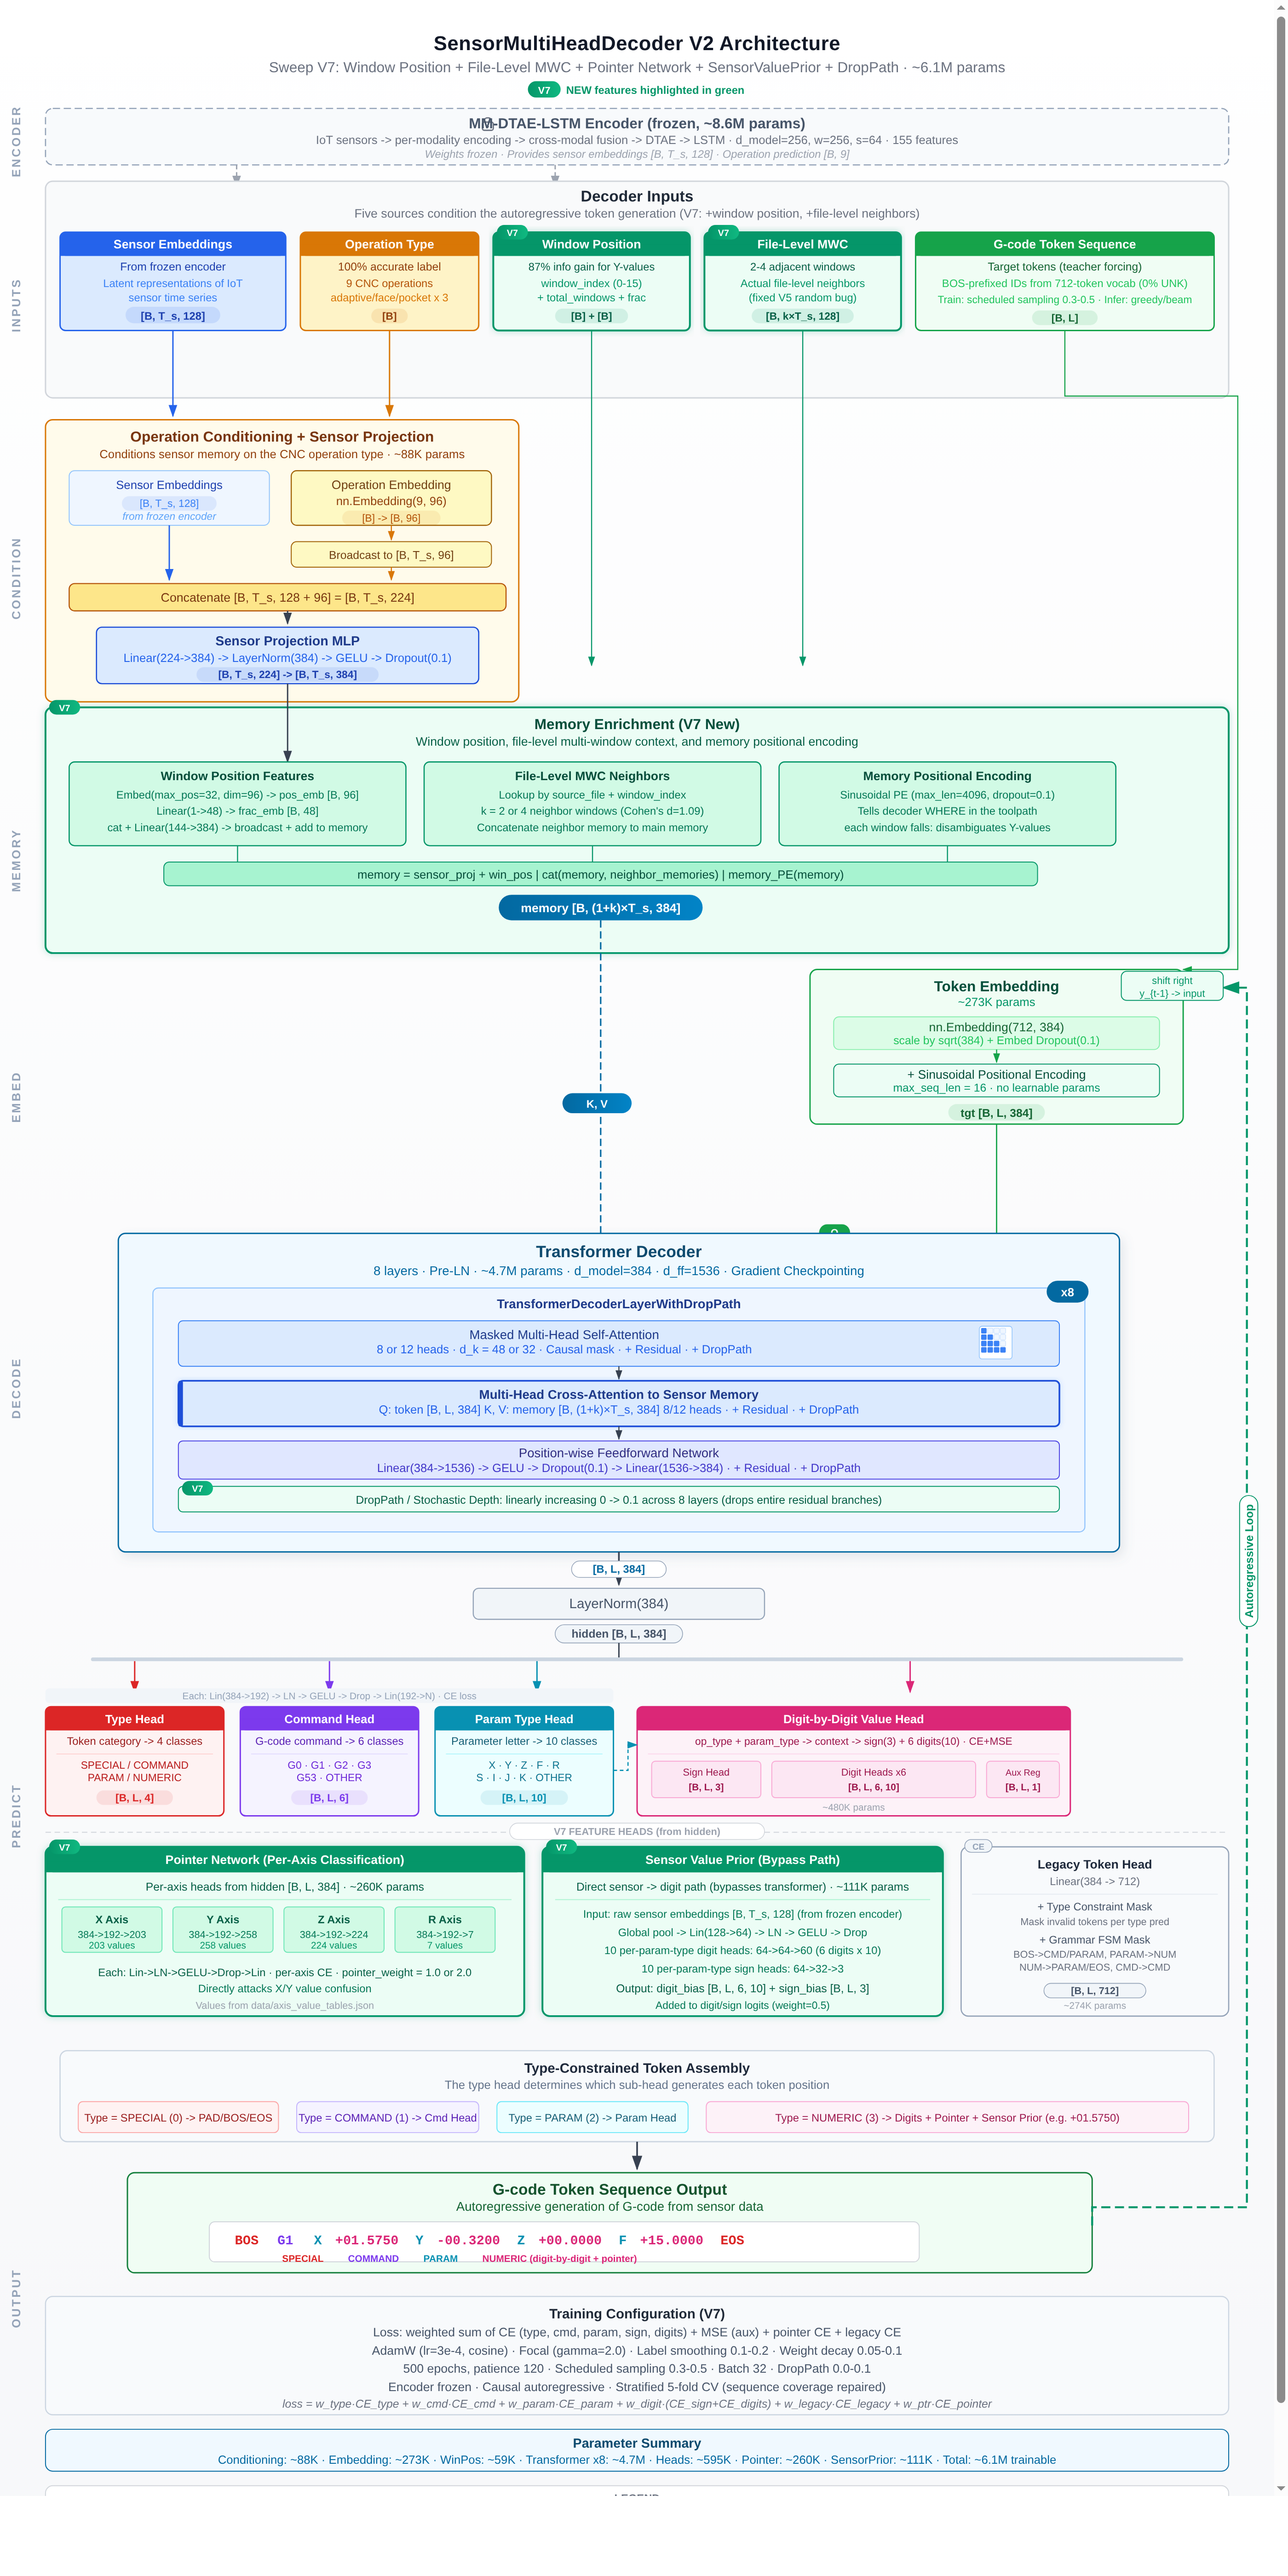
\includegraphics[width=0.42\textwidth,keepaspectratio]{figures/decoder_arch_v2.pdf}
\caption{System architecture. The frozen encoder (left) produces 256-dimensional memory from multi-modal sensor windows. The decoder (right) generates G-code tokens autoregressively via cross-attention, with hierarchical heads for type, command, parameter, and digit prediction.}
\label{fig:architecture}
\end{figure}

\subsection{Decoder Architecture}

The \decodername{} is a Transformer decoder~\cite{vaswani2017attention} with $d_\text{model} = 384$, $n_\text{layers} \in \{6, 8\}$, and $n_\text{heads} \in \{8, 12\}$. Each layer contains:

\begin{enumerate}[leftmargin=*]
    \item Masked self-attention over previously generated tokens
    \item Cross-attention over encoder memory $\mathbf{M}$
    \item Position-wise feed-forward network
\end{enumerate}

The encoder output ($d = 256$) is projected to the decoder dimension ($d = 384$) via a linear layer before cross-attention. The full decoder has 22.1M parameters, of which 85.8\% reside in the 8-layer Transformer (self-attention + cross-attention + feed-forward). Notably, the capacity ablations (Section~\ref{sec:ablations}) show that a 2-layer, $d{=}192$ variant with 3.0M parameters achieves 84.4\% sequence accuracy, suggesting the architecture is overparameterized for this task.

\subsection{Multi-Head Prediction}

Following the hierarchical token decomposition~\cite{grammar_paper}, prediction is decomposed into specialized heads:

\begin{itemize}[leftmargin=*]
    \item \textbf{Token type head}: 4-class classifier (Special, Command, Parameter, Numeric)
    \item \textbf{Command head}: 6-class classifier (G0, G1, G2, G3, G53, M30)
    \item \textbf{Parameter type head}: 9-class classifier (X, Y, Z, F, R, S, I, J, K)
    \item \textbf{Digit heads}: Per-position classifiers for sign (3-class) and 6 digits (10-class each)
    \item \textbf{Legacy token head}: Full 712-class vocabulary classifier
\end{itemize}

The legacy head provides a flat prediction baseline; the hierarchical heads provide structured decomposition. Both contribute to the training loss:

\begin{equation}
\mathcal{L} = \mathcal{L}_\text{legacy} + \mathcal{L}_\text{type} + \mathcal{L}_\text{cmd} + \mathcal{L}_\text{param} + w_d \sum_{i} \mathcal{L}_{d_i}
\label{eq:loss}
\end{equation}

\noindent All structural terms ($\mathcal{L}_\text{legacy}$, $\mathcal{L}_\text{type}$, $\mathcal{L}_\text{cmd}$, $\mathcal{L}_\text{param}$) are weighted at 1.0; only the digit weight $w_d$ is tuned, because digit prediction spans six positions and is the dominant source of numeric error. $w_d \in \{15, 20, 30\}$ was swept in V7; all three values produced identical best accuracy (Section~\ref{sec:rq4_minimum}). Each loss uses focal cross-entropy~\cite{focal_loss} with $\gamma = 2.0$ to handle class imbalance; class weights are uniform across heads. Label smoothing ($\alpha \in \{0.1, 0.2\}$) provides additional regularization.

\subsection{Grammar-Constrained Decoding}

At each generation step, a type-transition mask $M(\tau_{t-1}) \in \{0, -\infty\}^{|\mathcal{V}|}$ is applied to the legacy head logits based on the previous token's type~\cite{grammar_paper}:

\begin{equation}
    \tilde{\ell}^{(t)} = \ell^{(t)} + M(\tau_{t-1})
\end{equation}

For example, after a \textsc{Parameter} token, only \textsc{Numeric} tokens are valid; after \textsc{Numeric}, only \textsc{Parameter} or \textsc{EOS} are valid. Command-specific rules further constrain parameter selection (\eg, in this dataset's controller dialect, G0 rapid traverse does not use F; G2/G3 circular interpolation requires R for the radius-format arcs used here). These constraints guarantee syntactically valid output regardless of model confidence.

An important finding from our experiments (Section~\ref{sec:ablations}) is that grammar constraints' effectiveness depends on rule correctness. Initial rules that prohibited command-less sequences (where modal persistence makes the command implicit) \emph{hurt} performance by penalizing valid G-code. After fixing the rules to allow \textsc{BOS}$\to$\textsc{Parameter} and \textsc{Numeric}$\to$\textsc{Command} transitions, grammar constraints became beneficial for top configurations.

\subsection{Scheduled Sampling}

During training, the decoder uses teacher forcing with scheduled sampling~\cite{scheduled_sampling}: at each step, the ground-truth previous token is replaced with the model's own prediction with probability $p_\text{ss} \cdot \min(1, \text{epoch}/E)$, where $p_\text{ss} \in \{0.3, 0.5\}$ and $E$ is the total epochs. This bridges the train-test distribution gap for autoregressive models.

The base decoder described above processes one window at a time. The following section introduces features that extend its context beyond the individual window.

% ============================================================================
\section{Temporal Context Features}
\label{sec:v7_features}

The single most impactful architectural contribution is providing the decoder with temporal context beyond the individual sensor window.

\subsection{Memory Positional Encoding}

Sinusoidal positional encoding is added to the encoder memory $\mathbf{M}$ before cross-attention, telling the decoder \emph{where within the compressed sequence} each memory position falls. This is distinct from the standard decoder positional encoding (which tracks output token position) and provides spatial structure to the sensor representation.

\subsection{Multi-Window Context (MWC)}

A single 256-timestep window captures 64~seconds of machining at the $\sim$4~Hz aligned sampling rate. Three sampling regimes coexist in the data pipeline: the native LSM9DS1 IMU samples at 119~Hz (59.5~Hz Nyquist), the firmware-level RMS audio and environmental sensors sample at 10~Hz, and the final aligned rate after interpolation to the machine-status timeline is $\sim$4~Hz. The 400~Hz tooth-passing frequency exceeds every one of these Nyquist limits and is not recoverable from any of the recorded streams. The question is therefore not whether tooth-passing harmonics survive---they do not---but whether any signal that \emph{does} survive carries toolpath-discriminative information. The encoder paper~\cite{encoder_paper} argues on physical grounds that discriminative content lives in low-frequency structural-mode vibration (1--50~Hz), acceleration transients at toolpath direction changes, and operation-specific trajectory envelopes---frequencies that are either captured natively at 119~Hz or, for trajectory envelopes, present at any rate above the motion bandwidth ($\sim$1~Hz). Figure~\ref{fig:psd_aligned} shows empirical power spectral densities at the 4~Hz aligned rate for three representative toolpaths and confirms that meaningful spectral structure exists in the DC--2~Hz band: face milling shows periodic structure corresponding to step-over passes, pocket machining shows burst-like low-frequency energy, and adaptive clearing shows broadband activity consistent with its continuous direction reversals. The 4~Hz aligned rate is thus a deliberate choice that preserves trajectory-envelope information at the cost of high-frequency cutting dynamics---a trade we accept for this work but that would need revisiting for applications targeting sub-second fault detection or chatter characterization.

\begin{figure}[htbp]
\centering
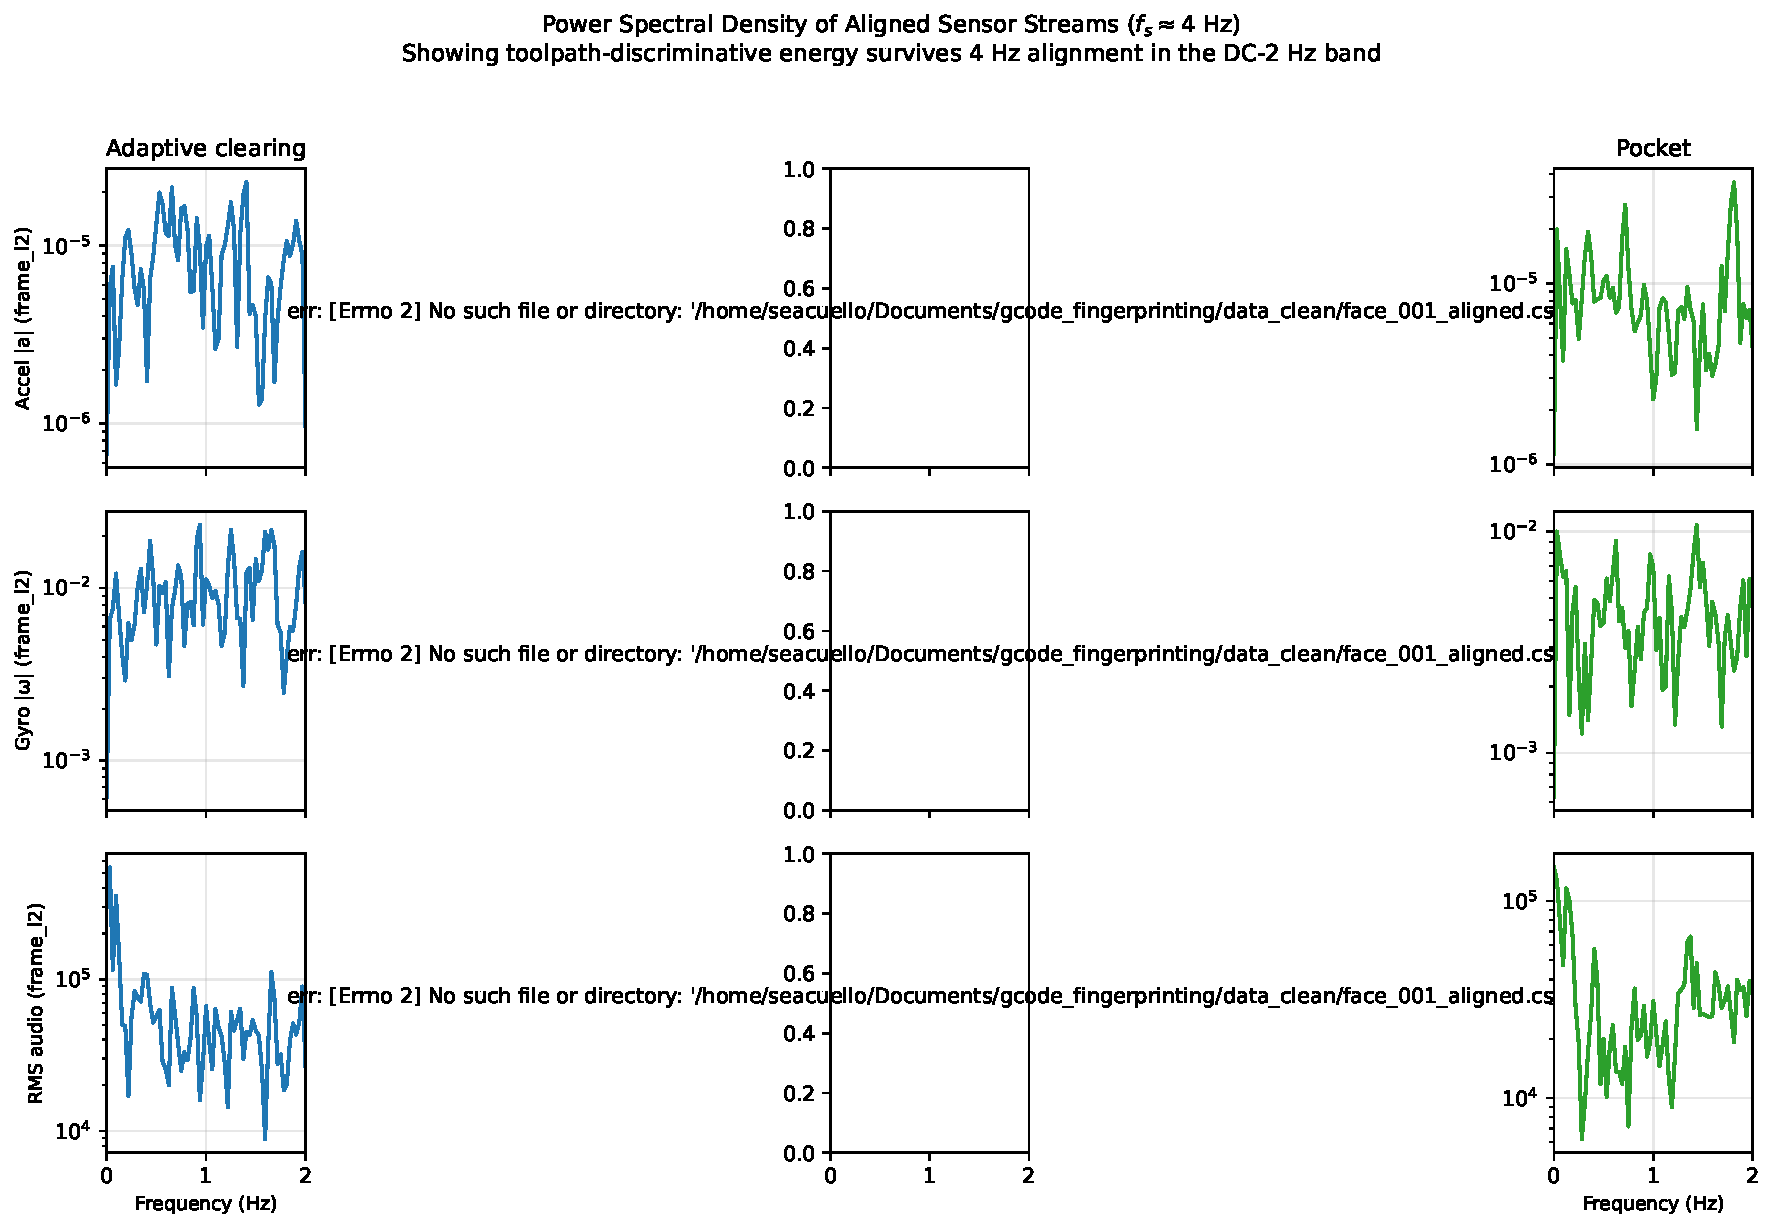
\includegraphics[width=\textwidth]{figures/psd_aligned_sensors.pdf}
\caption{Power spectral density of three representative sensor channels (accelerometer magnitude, gyroscope magnitude, RMS audio from the frame\_l2 board) for three representative toolpath files at the 4~Hz aligned sampling rate. Distinct spectral signatures survive the alignment despite the loss of the 400~Hz tooth-passing frequency and 59.5~Hz IMU Nyquist.}
\label{fig:psd_aligned}
\end{figure} Many G-code distinctions---particularly Y-axis coordinate values that differ between successive passes---require context spanning multiple windows. Multi-window context concatenates encoder memories from adjacent windows within the same source file:

\begin{equation}
    \mathbf{M}_\text{ctx} = [\mathbf{M}_{i-k}, \ldots, \mathbf{M}_i, \ldots, \mathbf{M}_{i+k}]
\end{equation}

\noindent where $k \in \{1, 2\}$ is the context radius. Critically, neighbors must come from the \emph{same source file} (same physical operation recording) and be ordered by window index within that file. Early implementations (V5--V6) used index-based neighbors after \texttt{DataLoader} shuffle, inadvertently producing random windows from unrelated files---a bug that nonetheless showed positive signal (V5 Cohen's $d = 1.09$ for the combined MWC + memory positional encoding effect, measured with the buggy random neighbors). Correcting to file-level neighbors in V7 reduced the MWC-specific contribution to $-$2.8~pp (Table~\ref{tab:ablations}), indicating that much of the V5 effect was attributable to window position metadata rather than temporal context per se.

\subsection{Window Position Embedding}

Each window is identified by its position within the source file: $(\text{window\_index}, \text{total\_windows})$. A discrete embedding for the window index and a continuous projection of the normalized position $(\text{index}/\text{total})$ are concatenated and added to the decoder's initial hidden state.

Window position provides 57.8\% normalized information gain for Y-axis step-over value disambiguation, computed as the reduction in conditional entropy $H(Y|\text{position})$ relative to the marginal entropy $H(Y)$ over all training windows containing Y-axis coordinates. The relationship is structured but not deterministic: $Y = 0.1755$ is the most common Y-value at positions 0--1 (34--38\% of windows at those positions), and $Y = 2.9132$ is dominant at position~2 (52--93\% depending on fold). The partial correlation reflects the diversity of toolpath strategies and operating conditions in the dataset: each strategy uses different Y-coordinate progressions. Nonetheless, the 57.8\% entropy reduction confirms that window position provides substantial disambiguation. This positional information is encoded in the file structure but invisible to a single-window encoder---the sensor dynamics during each pass are governed by cutting conditions (depth, feed, engagement), not the table's lateral position. Window position was the single highest-impact feature, blocked in V5--V6 due to missing metadata in the preprocessed NPZ files, and enabled in V7 after re-processing the full data pipeline from raw sensor CSVs.

\subsection{Pointer Network for Per-Axis Classification}

A pointer network was also tested with per-axis classification heads (X: 203 values, Y: 258, Z: 224, R: 7) to replace the flat 712-class legacy head. Each head is a small MLP predicting only the values relevant to the current axis. This feature showed no benefit in V7 (Table~\ref{tab:v7_features}) and was locked OFF, suggesting that the legacy head's shared representation is sufficient once the preprocessing is correct.

% ============================================================================
\section{Experimental Setup}
\label{sec:experimental}

\subsection{Dataset}

The dataset is the same as~\cite{encoder_paper}: 120 cleaned operation files from a Bantam Tools Explorer\texttrademark{} desktop CNC milling machine. The machine is instrumented with six Arduino Nano 33 BLE Sense Lite sensor boards (Table~\ref{tab:sensors}) spanning three structural locations---frame (3 boards), spindle (1), and bed (2), shown in Figure~\ref{fig:sensor_placement}---plus machine-level electrical monitoring via MCCDAQ. Each board integrates a 9-axis IMU (LSM9DS1: accelerometer, gyroscope, magnetometer at 119~Hz native), environmental sensors (LPS22HB pressure/temperature, APDS-9960 proximity at 10~Hz), and a PDM microphone computing RMS audio at the firmware level. All streams are aggregated via USB serial on a Raspberry Pi~4, then interpolated and aligned to the machine status timeline at an effective rate of $\sim$4~Hz for G-code labeling. Full instrumentation details, sensor placement photographs, and data cleaning procedures are described in~\cite{encoder_paper}.

\begin{table}[htbp]
\centering
\caption{Sensor Configuration (6 Boards $\times$ 17 Channels + 8 Electrical = 110 Features)}
\label{tab:sensors}
\small
\begin{tabular}{@{}llcc@{}}
\toprule
\textbf{Modality} & \textbf{Channels} & \textbf{Per Board} & \textbf{$\times$6} \\
\midrule
Accelerometer & Ax, Ay, Az & 3 & 18 \\
Gyroscope     & Gx, Gy, Gz & 3 & 18 \\
Magnetometer  & Mx, My, Mz & 3 & 18 \\
Pressure      & Barometric  & 1 & 6 \\
Temperature   & Ambient     & 1 & 6 \\
Proximity     & APDS-9960   & 1 & 6 \\
Color         & R, G, B, A  & 4 & 24 \\
RMS Audio     & PDM mic     & 1 & 6 \\
\midrule
\multicolumn{3}{@{}l}{+ Machine electrical (voltage, current, spindle)} & 8 \\
\midrule
\multicolumn{3}{@{}l}{\textbf{Total}} & \textbf{110} \\
\bottomrule
\end{tabular}
\normalsize
\end{table}

\begin{figure}[htbp]
\centering
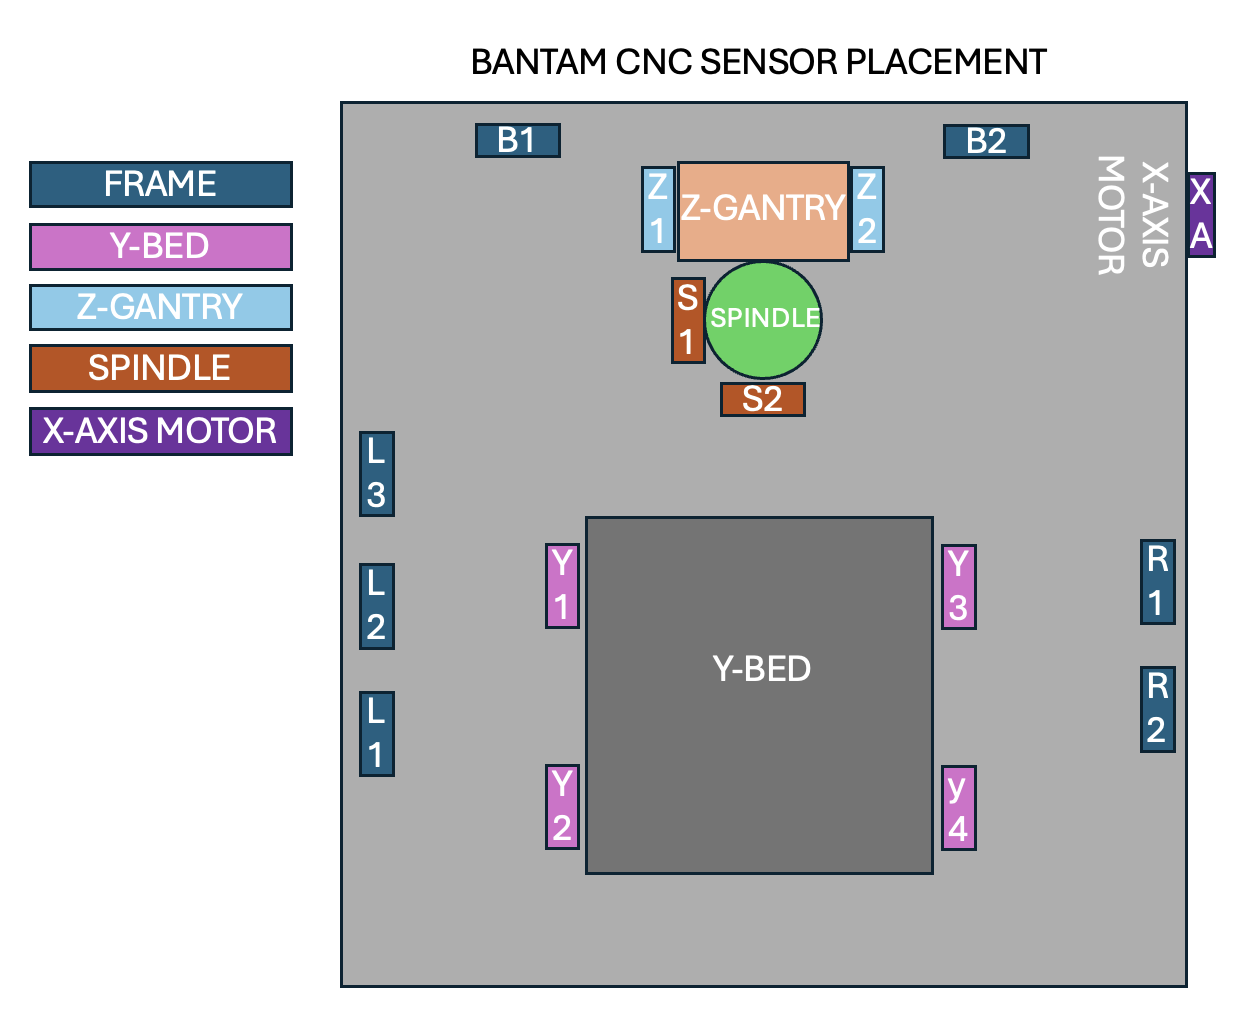
\includegraphics[width=0.85\textwidth]{figures/sensor_placement_schematic.png}
\caption{Sensor placement schematic showing six Arduino boards distributed across the machine frame (3), spindle (1), and bed (2), providing spatial diversity across the primary vibration transmission paths.}
\label{fig:sensor_placement}
\end{figure}

All operations used a 2-flute HSS flat endmill (1/4\textquotedbl{} / 6.35~mm diameter) at 12{,}000~RPM (tooth-passing frequency $f_t = 400$~Hz) and 1{,}016~mm/min feed rate. Face milling and pocketing used a 3.81~mm stepover (60\% of tool diameter), while adaptive clearing used trochoidal toolpaths with 10--25\% radial engagement. These are typical parameters for hobby-grade desktop CNC milling. Active-cutting trials machined TIVAR UHMW-PE (ultra-high molecular weight polyethylene) at 0.635~mm axial depth. This soft polymer was chosen for reproducible, low-variation cutting forces; metals would produce fundamentally different force, thermal, and acoustic signatures.

The dataset spans 9 operation classes (Table~\ref{tab:classes}): three toolpath strategies (Figure~\ref{fig:toolpaths}) $\times$ three operating conditions.

\begin{table}[htbp]
\centering
\caption{Nine Operation Classes (3 Toolpaths $\times$ 3 Conditions)}
\label{tab:classes}
\small
\begin{tabular}{@{}llcc@{}}
\toprule
\textbf{Toolpath} & \textbf{Condition} & \textbf{Label} & \textbf{Files} \\
\midrule
Adaptive clearing & Air-cut       & adaptive        & 20 \\
Adaptive clearing & Active-cut    & adaptive150025  & 17 \\
Adaptive clearing & Damaged       & damageadaptive  & 5 \\
Face milling      & Air-cut       & face            & 16 \\
Face milling      & Active-cut    & face150025      & 15 \\
Face milling      & Damaged       & damageface      & 4 \\
Pocket machining  & Air-cut       & pocket          & 19 \\
Pocket machining  & Active-cut    & pocket150025    & 19 \\
Pocket machining  & Damaged       & damagepocket    & 5 \\
\midrule
\multicolumn{3}{@{}l}{\textbf{Total}} & \textbf{120} \\
\bottomrule
\end{tabular}
\normalsize
\end{table}

\begin{figure}[htbp]
\centering
\begin{tabular}{@{}ccc@{}}
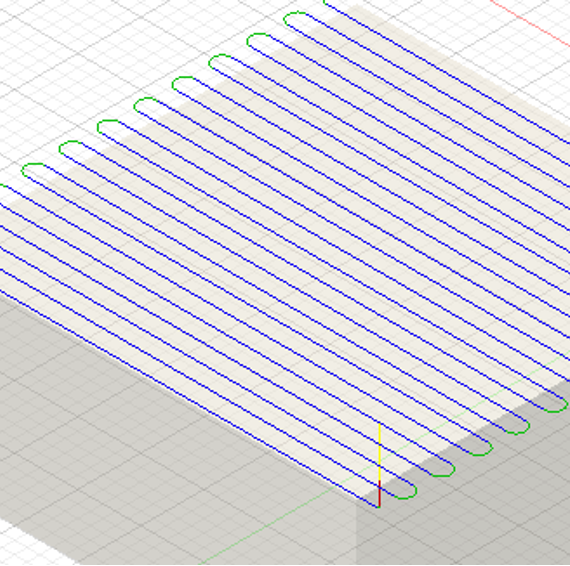
\includegraphics[width=0.30\textwidth]{figures/toolpath_face.png} &
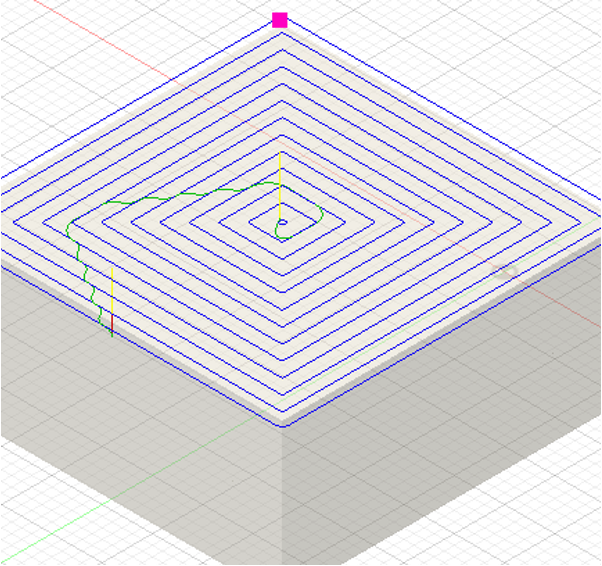
\includegraphics[width=0.30\textwidth]{figures/toolpath_pocket.png} &
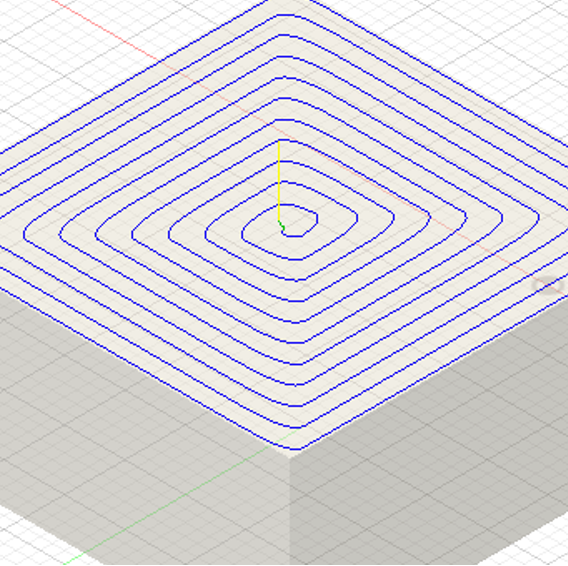
\includegraphics[width=0.30\textwidth]{figures/toolpath_adaptive.png} \\
{\small (a) Face milling} & {\small (b) Pocket} & {\small (c) Adaptive}
\end{tabular}
\caption{CAM toolpath strategies: (a)~face milling sweeps in parallel linear passes with periodic step-over transitions; (b)~pocket machining alternates between axial plunges and lateral clearing passes; (c)~adaptive clearing follows trochoidal paths maintaining near-constant radial engagement (10--25\% of tool diameter) with frequent direction reversals.}
\label{fig:toolpaths}
\end{figure}

The three conditions are: \textbf{air-cutting} (spindle running, no material engagement---machine dynamics only), \textbf{active cutting} (0.635~mm depth in UHMW-PE, adding cutting forces and chip formation signatures), and \textbf{damaged spindle} (air-cutting with one drive band removed, inducing spindle runout that simulates one specific drive-train degradation mode). We emphasize that this damaged condition is a single simulated fault; real-world spindle health issues include bearing wear, unbalance, and thermal growth, whose sensor signatures may differ from the drive-band removal we study. The ``150025'' suffix in class labels encodes the 0.025" depth-of-cut parameter from the CAM configuration.

With window size $W = 256$ timesteps (64~seconds at $\sim$4~Hz) and stride 64, the 120 files produce 545 sensor windows. Each window maps to a single G-code line. Across all folds, 34 unique G-code target sequences exist (27 per fold after stratified splitting), with a highly imbalanced distribution: the most common sequence (\texttt{G1 X-0.1254}) covers 20\% of windows, while 17 sequences have fewer than 20 windows each.

Figure~\ref{fig:timeseries} shows representative sensor traces from the three toolpath strategies. Adaptive clearing produces irregular, high-frequency direction changes; face milling shows periodic step-over transitions; pocket machining exhibits burst-like plunge--clear dynamics. These distinct temporal patterns are what the encoder compresses into the 256-dimensional embeddings that serve as decoder input. Figure~\ref{fig:encoder_pca} confirms that the encoder separates operation classes in embedding space, with clear clustering by toolpath strategy and subclustering by operating condition.

\begin{figure}[H]
\centering
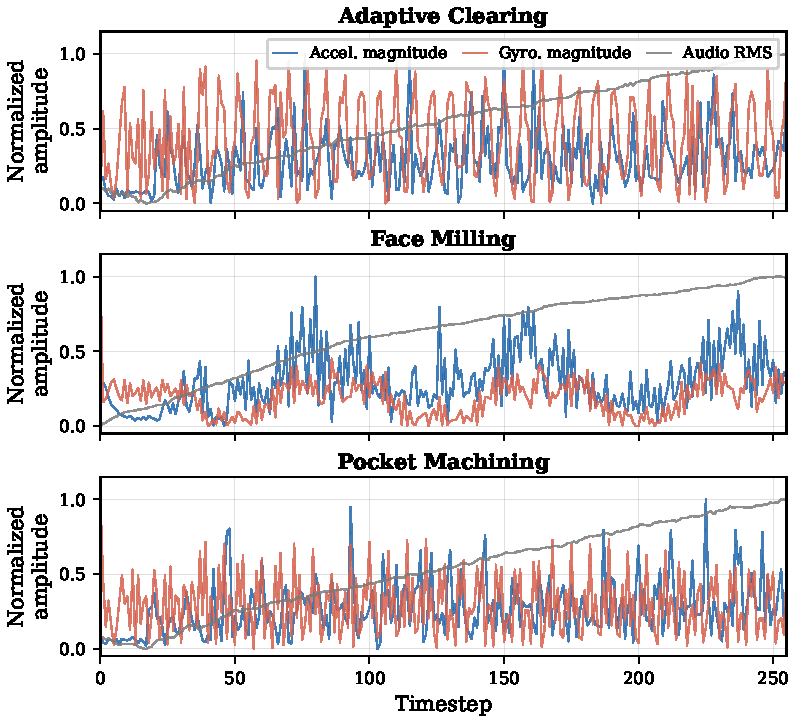
\includegraphics[width=0.85\textwidth]{figures/sensor_timeseries_comparison.pdf}
\caption{Raw sensor traces for three toolpath strategies (accelerometer magnitude, gyroscope magnitude, RMS audio from one sensor board). Adaptive clearing shows irregular direction changes, face milling shows periodic step-overs, and pocket machining shows burst-like plunge--clear dynamics.}
\label{fig:timeseries}
\end{figure}

\begin{figure}[H]
\centering
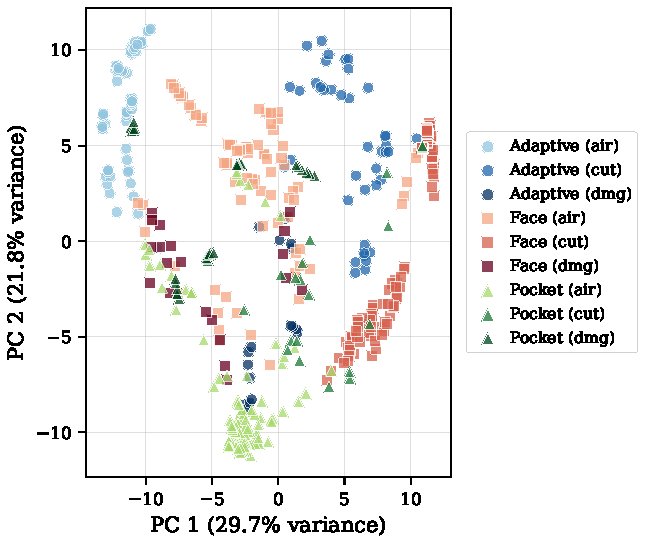
\includegraphics[width=0.75\textwidth]{figures/encoder_embedding_pca.pdf}
\caption{PCA of encoder embeddings (mean-pooled over 256 timesteps) for all 552 test windows across five folds. PC1--PC2 explain 51.5\% of variance. Operations cluster by toolpath strategy (adaptive/face/pocket) with subclusters by condition (air-cut/active/damaged).}
\label{fig:encoder_pca}
\end{figure}

\subsection{Preprocessing and Cross-Validation}

Five-fold file-level stratified cross-validation prevents window-level data leakage. Each fold allocates 69--75 files for training, 21--26 for validation, and 21--26 for testing. A sequence coverage repair algorithm swaps files between folds to ensure all G-code sequences in the validation and test sets also appear in training, eliminating impossible predictions.

Sensor features are robust-scaled (per-fold) using training statistics only. G-code targets are tokenized using the hybrid tokenizer~\cite{grammar_paper} with a 712-token vocabulary.

\subsection{Training Configuration}

All experiments use AdamW optimization with cosine annealing and linear warmup. Key fixed hyperparameters (determined through progressive sweeps): learning rate $3 \times 10^{-4}$, $d_\text{model} = 384$, batch size 32, dropout 0.1, focal $\gamma = 2.0$. Gradient clipping at 1.0 prevents instability. All sweeps ran on a workstation with two NVIDIA RTX~A6000 GPUs (48~GB each), using Ray Tune for parallel trial scheduling (6--14 concurrent trials). Table~\ref{tab:compute} summarizes the computational budget.

\begin{table}[htbp]
\centering
\caption{Computational Budget (2$\times$ NVIDIA RTX A6000). Approximately 2{,}000 GPU-hours over two weeks, with individual trials requiring 10--45 minutes.}
\label{tab:compute}
\small
\begin{tabular}{@{}lrrc@{}}
\toprule
\textbf{Experiment} & \textbf{Runs} & \textbf{GPU-hrs} & \textbf{Min/run} \\
\midrule
V1--V2 sweeps      & 1{,}892 & 390  & 10--15 \\
V3--V6 sweeps      & 2{,}733 & 1{,}370 & 25--35 \\
V7 sweep            & 157   & 92   & 35 \\
5-fold retrain (5 seeds) & 25 & 13 & 30 \\
Architecture ablations & 60 & 30  & 30 \\
Modality ablations  & 45    & 28   & 35 \\
Window ablations    & 10    & 5    & 30 \\
Baselines           & 35    & 5    & 8 \\
Encoder training    & 50    & 2    & 2 \\
\midrule
\textbf{Total}      & \textbf{5{,}007} & $\sim$\textbf{1{,}935} & --- \\
\bottomrule
\end{tabular}
\normalsize
\end{table}

\subsection{Sweep Methodology}

Rather than a single large sweep, we conducted seven progressive sweeps (V1--V7), each building on insights from the previous:

\begin{enumerate}[leftmargin=*]
    \item \textbf{V1} (1{,}000 trials): Baseline architecture search. 100 epochs, single fold.
    \item \textbf{V2} (892 trials): Wider architectures, higher digit weights. 250 epochs.
    \item \textbf{V3} (320 trials): Cross-validation, longer training. 500 epochs, 5 folds.
    \item \textbf{V4} (352 trials): +hierarchical conditioning, +memory positional encoding.
    \item \textbf{V5} (1{,}568 trials): +grammar constraints, +multi-window context.
    \item \textbf{V6} (493 trials): Fixed grammar rules, +oversampling, +window dropout.
    \item \textbf{V7} (157 trials): Re-preprocessed data from raw CSVs; +window position, +file-level MWC, +pointer network, +sensor prior.
\end{enumerate}

The progressive approach locks converged hyperparameters early (\eg, $d_\text{model} = 384$ locked after V2, focal $\gamma = 2.0$ after V3) and introduces new features in controlled batches, enabling causal attribution of accuracy improvements. With the experimental framework established, the following section presents results addressing each research question.

% ============================================================================
\section{Results}
\label{sec:results}

This section presents results addressing the four research questions in order: reconstruction accuracy (RQ1, Section~\ref{sec:rq1_accuracy}), the relative contribution of architecture versus data handling (RQ2, Section~\ref{sec:rq3_pipeline}), sensor modality importance (RQ3, Section~\ref{sec:rq2_modality}), and minimum viable configuration for deployment (RQ4, Section~\ref{sec:rq4_minimum}). Throughout, we report metrics from the final V7 sweep (157 trials, 5-fold cross-validation) unless otherwise noted. The sweep progression from V1 through V7 and additional feature analyses are detailed in Appendix~\ref{sec:appendix_sweep}.

An important caveat up front: a position-based lookup table achieves 90.4\% sequence accuracy on this dataset without any model, outperforming the decoder's 86.1\% (Table~\ref{tab:baselines}). The decoder's contribution is not raw accuracy on the training geometry---a lookup table achieves that more efficiently---but rather a learned sensor-to-G-code mapping that generalizes beyond the training file structure and provides structured predictions suitable for anomaly detection.

\subsection{Reconstruction Accuracy (RQ1)}
\label{sec:rq1_accuracy}

Table~\ref{tab:v7_5fold} reports the per-fold results for the best V7 configuration, retrained from scratch on each fold with 5 random seeds per fold (best seed selected).

\begin{table}[htbp]
\centering
\caption{V7 Per-Fold Test Results (\%). Each fold was retrained with 5 random seeds; we report the mean-of-seeds as the primary per-fold value and the best-of-seeds for comparison. Std reflects fold-to-fold variance; within-fold seed std averages 1.4~pp. Fold~1 is consistently the hardest---an encoder-representation limitation not addressed by the decoder.}
\label{tab:v7_5fold}
\small
\begin{tabular}{@{}lcccccc@{}}
\toprule
& \textbf{Seq (mean)} & \textbf{Seq (best)} & \textbf{Tok} & \textbf{Num} & \textbf{Cmd} & \textbf{Param} \\
\midrule
Fold 1 & 69.4 & 71.2 & 87.6 & 80.4 & 96.3 & 92.9 \\
Fold 2 & 88.3 & 89.4 & 96.3 & 93.7 & 97.6 & 98.4 \\
Fold 3 & 87.4 & 88.7 & 95.6 & 93.0 & 100.0 & 98.1 \\
Fold 4 & 88.0 & 89.8 & 96.3 & 93.3 & 97.7 & 98.5 \\
Fold 5 & 89.5 & 91.4 & 97.2 & 93.8 & 100.0 & 98.2 \\
\midrule
\textbf{Mean} & \textbf{84.5} & \textbf{86.1} & \textbf{94.6} & \textbf{90.8} & \textbf{98.3} & \textbf{97.2} \\
Std          & 8.5           & 8.4           & 4.1          & 5.7          & 1.7          & 2.4 \\
\bottomrule
\end{tabular}
\normalsize
\end{table}

The decoder achieves \textbf{84.5\% mean cross-fold sequence accuracy} (single-seed average, 5 seeds per fold). The best-of-5-seeds figure is 86.1\% and is reported alongside for comparison, but the single-seed mean is the more honest estimator of deployable performance because it does not include seed-selection bias. Token accuracy is 94.6\% and command accuracy is 98.3\%---the structural components of G-code (motion commands and parameter addresses) are near-perfectly reconstructed; the remaining errors concentrate in numeric coordinate values, particularly Y-axis step-over positions (Section~\ref{sec:errors}).

\paragraph{Uncertainty on headline numbers.} With only $n=5$ folds, Gaussian standard errors are not reliable summaries of uncertainty. A paired fold-level bootstrap (10{,}000 resamples) gives the following 95\% confidence intervals: mean-of-seeds sequence accuracy 84.5\%, 95\%~CI [76.8, 88.8]; best-of-seeds 86.1\%, 95\%~CI [78.5, 90.5]; sensor-only (window position removed) 62.3\%, 95\%~CI [57.1, 67.4]; physics-ceiling gap 22.2~pp, 95\%~CI [17.9, 27.4]. The wide CIs reflect the limited statistical power of 5-fold CV on a 545-window dataset; the gap CI nonetheless excludes zero with comfortable margin, confirming that the physics-ceiling effect is robust to fold resampling even though individual accuracy numbers are not tightly estimated. All other quantitative claims in this paper should be read under similar caveats: point estimates are reliable to within $\pm$5~pp, and we recommend interpreting differences smaller than the widest individual CI (about 6~pp for the best-of-seeds headline) as qualitative rather than quantitative.

Teacher-forced and greedy autoregressive decoding produce identical aggregate sequence accuracy on all five folds, and beam search ($k \in \{3, 5\}$) provides no further improvement. Per-item inspection reveals that individual predictions do differ across decode modes on 7.1\% of test windows (median across folds; 18\% on the hardest fold), but those differences are symmetric---one decode mode gets right what another gets wrong, in equal counts---so aggregate accuracy is unchanged. This is the signature of representational ambiguity at the sensor level rather than search error in the decoder: any reasonable decoding strategy fails on the same set of physically ambiguous windows, just on slightly different subsets. The scheduled sampling training regime ($p_\text{ss} = 0.5$) further closes the teacher-forcing gap, so the exposure-bias concern that usually distinguishes teacher-forced evaluation from greedy decoding is empirically absent here.

Table~\ref{tab:per_class} reports per-operation accuracy, computed from the V7 best configuration with teacher-forced decoding across all 552 test windows.

\begin{table}[htbp]
\centering
\caption{Reconstruction Accuracy by Operation Class (V7 Best Config, 552 Test Windows)}
\label{tab:per_class}
\small
\begin{tabular}{@{}llcccc@{}}
\toprule
\textbf{Toolpath} & \textbf{Condition} & \textbf{Windows} & \textbf{Seq.} & \textbf{Tok.} \\
\midrule
Adaptive & Air-cut  & 40  & 100.0\% & 100.0\% \\
Adaptive & Active   & 68  & 91.2\%  & 95.6\% \\
Adaptive & Damaged  & 20  & 100.0\% & 100.0\% \\
Face     & Air-cut  & 144 & 100.0\% & 100.0\% \\
Face     & Active   & 87  & 72.4\%  & 89.6\% \\
Face     & Damaged  & 20  & 90.0\%  & 96.7\% \\
Pocket   & Air-cut  & 19  & 94.7\%  & 99.1\% \\
Pocket   & Active   & 124 & 71.0\%  & 85.9\% \\
Pocket   & Damaged  & 30  & 60.0\%  & 77.6\% \\
\midrule
\multicolumn{2}{@{}l}{\textbf{Overall}} & \textbf{552} & \textbf{85.3\%}$^\dagger$ & \textbf{93.5\%} \\
\bottomrule
\multicolumn{5}{@{}l}{\scriptsize $^\dagger$Pooled across all windows; differs from the 86.1\% mean-of-folds}\\
\multicolumn{5}{@{}l}{\scriptsize (Table~\ref{tab:v7_5fold}) because fold sizes are unequal and the hardest}\\
\multicolumn{5}{@{}l}{\scriptsize fold (Fold~1, 71.2\%) has the most test windows (132 of 552).}
\end{tabular}
\normalsize
\end{table}

Reconstruction difficulty varies systematically with both toolpath strategy and operating condition. Air-cutting (no material engagement) is near-perfect across all three strategies (99.5\% mean sequence accuracy): machine dynamics are highly repeatable when no cutting forces are present. Active cutting (76.3\%) and damaged spindle (80.0\%) are 6--24~pp harder because cutting-force variability from chip formation and spindle runout introduce noise that obscures the coordinate-level signal. By strategy, adaptive clearing (95.3\%) and face milling (89.6\%) outperform pocket machining (71.7\%). Pocket air-cutting remains high (94.7\%) because without material, the plunge--clear geometry still produces distinctive motion dynamics. Active pocket drops to 71.0\% because chip formation forces vary with instantaneous radial engagement during lateral clearing passes, adding stochastic noise to the sensor signal that obscures the coordinate-level information the decoder needs for exact reconstruction.

\paragraph{Fold variance.} V7's data pipeline fixes reduced the cross-fold spread from 26.3~pp (V6) to 17.9~pp and reordered fold difficulty entirely: Fold~5, previously the weakest (52.7\% in V6), became the strongest (91.4\% in V7) because window position metadata resolved the Y-axis step-over ambiguity that disproportionately affected that fold's test distribution. Fold~1 remains the hardest (71--74\% across configurations), suggesting that its file combinations contain toolpaths with inherently ambiguous sensor signatures. The full fold-by-sweep comparison is in Table~\ref{tab:folds} (Appendix~\ref{sec:appendix_sweep}).

\begin{figure}[htbp]
\centering
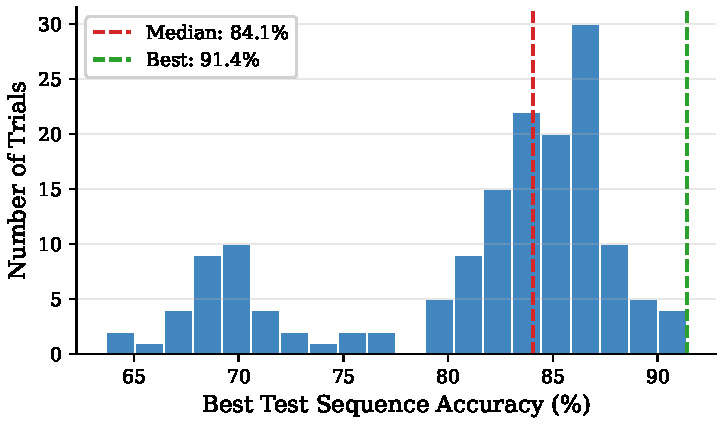
\includegraphics[width=\textwidth]{figures/v7_distribution.pdf}
\caption{Distribution of test sequence accuracy across all 157 V7 trials. The V7 median (84.1\%) exceeds V5's best accuracy on four of five individual folds (63.6\%, 81.0\%, 79.0\%, 65.6\%), indicating that data pipeline correctness yields more robust performance than architecture search.}
\label{fig:v7_distribution}
\end{figure}

Robustness is best captured by the \emph{median}: 84.1\% median sequence accuracy versus 33.4\% (V5) and 48.4\% (V6) (Figure~\ref{fig:v7_distribution}). The data pipeline fixes made the decoder robust to hyperparameter choices: nearly every configuration now produces a viable model, whereas in V5 only the top 10\% of configurations exceeded 80\%.

\paragraph{Statistical significance.} The Wilcoxon signed-rank test yields $p = 0.0625$ for both V7~vs.~V5 and V7~vs.~V6 (Table~\ref{tab:stats}). While this narrowly misses the conventional $\alpha = 0.05$ threshold, it is the \emph{minimum possible $p$-value} with $n = 5$ paired samples when all differences are in the same direction---meaning V7 improved every fold for both comparisons. The practical significance is clear: V7 reduced the standard deviation from 10.0 (V5) to 7.2 while simultaneously raising the mean by 10.9 percentage points.

\begin{table}[htbp]
\centering
\caption{Best-Per-Fold Sequence Accuracy: Mean $\pm$ Std (\%). Wilcoxon $p = 0.0625$ is the minimum possible with $n{=}5$ paired samples when all differences are positive.}
\label{tab:stats}
\small
\begin{tabular}{@{}lccc@{}}
\toprule
& \textbf{Mean $\pm$ Std} & \textbf{Min--Max} & \textbf{vs.\ V7 $p$} \\
\midrule
V5 & $75.1 \pm 10.0$ & 63.6--86.4 & 0.0625 \\
V6 & $66.0 \pm 10.4$ & 52.7--79.0 & 0.0625 \\
\textbf{V7} & $\mathbf{86.1 \pm 8.4}$ & \textbf{71.2--91.4} & --- \\
\bottomrule
\multicolumn{4}{@{}l}{\scriptsize Wilcoxon signed-rank test (paired by fold). With $n{=}5$ paired}\\
\multicolumn{4}{@{}l}{\scriptsize samples, $p{=}0.0625$ is the minimum achievable $p$-value when all}\\
\multicolumn{4}{@{}l}{\scriptsize differences are positive (all 5 folds improved V5$\to$V7 and V6$\to$V7).}
\end{tabular}
\normalsize
\end{table}

\subsection{Architecture vs.\ Data Pipeline (RQ2)}
\label{sec:rq3_pipeline}

A central finding of this work is that data-handling correctness dominates architectural complexity for reconstruction accuracy. We present evidence from baselines, controlled ablations, and the sweep history.

\subsubsection{Baseline Comparisons}

To quantify the decoder's contribution over simpler approaches, we compare against a progression of baselines (Table~\ref{tab:baselines}).

\begin{table}[htbp]
\centering
\caption{Baseline Comparison (mean $\pm$ std across 5 folds). The position-based lookup table (1A) outperforms the decoder on raw accuracy; model-based baselines (1B--1D) perform 33--40~pp worse.}
\label{tab:baselines}
\small
\begin{tabular}{@{}lcccc@{}}
\toprule
\textbf{Method} & \textbf{Seq.} & \textbf{Num.} & \textbf{Cmd.} & \textbf{Tok.} \\
\midrule
1A.\ Majority lookup$^\ast$     & $\mathit{90.4 \pm 5.6}$ & $\mathit{92.2 \pm 5.0}$ & $\mathit{98.7 \pm 1.1}$ & $\mathit{96.3 \pm 2.4}$ \\
1B.\ 1-NN retrieval            & $46.5 \pm 4.1$ & $52.5 \pm 6.2$ & $92.0 \pm 6.1$ & $75.2 \pm 4.3$ \\
1B.\ 5-NN retrieval            & $50.3 \pm 3.6$ & $57.2 \pm 4.7$ & $93.1 \pm 6.1$ & $78.1 \pm 5.1$ \\
1C.\ MLP (1-layer)             & $48.9 \pm 4.5$ & $55.3 \pm 6.0$ & $92.9 \pm 6.4$ & $77.8 \pm 3.7$ \\
1C.\ MLP (2-layer)             & $47.4 \pm 3.3$ & $53.2 \pm 5.1$ & $94.0 \pm 4.5$ & $77.2 \pm 4.4$ \\
1D.\ Random Forest             & $53.5 \pm 3.5$ & $60.9 \pm 3.4$ & $93.7 \pm 6.7$ & $80.2 \pm 4.0$ \\
1D.\ XGBoost                   & $53.0 \pm 5.3$ & $60.0 \pm 5.5$ & $94.1 \pm 5.9$ & $79.5 \pm 4.5$ \\
1E.\ 34-class MLP (sensor-only)$^\ddag$ & $49.6 \pm 4.9$ & --- & --- & --- \\
1E.\ 34-class MLP (+window pos.)$^\ddag$ & $77.5 \pm 8.1$ & --- & --- & --- \\
\midrule
\textbf{V7 decoder (mean-of-seeds)} & $\mathbf{84.5 \pm 8.5}$ & $\mathbf{90.8 \pm 5.7}$ & $\mathbf{98.3 \pm 1.7}$ & $\mathbf{94.6 \pm 4.1}$ \\
V7 decoder (best-of-seeds)          & $86.1 \pm 8.4$          & $91.3 \pm 5.4$          & $98.1 \pm 1.9$          & $94.9 \pm 4.2$ \\
\bottomrule
\multicolumn{5}{@{}l}{\scriptsize $^\ast$Position$\to$majority G-code lookup table, no model.}\\
\multicolumn{5}{@{}l}{\scriptsize $^\ddag$1E: MLP($\to$256$\to$128$\to$34) on mean-pooled encoder memory, 34-way}\\
\multicolumn{5}{@{}l}{\scriptsize sequence classification. The two rows differ only by whether the window}\\
\multicolumn{5}{@{}l}{\scriptsize position features (index, total) are appended to the input. This confirms}\\
\multicolumn{5}{@{}l}{\scriptsize that a simple classifier can extract most of the position signal; the}\\
\multicolumn{5}{@{}l}{\scriptsize decoder's 7~pp improvement over 1E(+pos) reflects the value of autoregressive}\\
\multicolumn{5}{@{}l}{\scriptsize grammar decomposition on top of the same features.}\\
\multicolumn{5}{@{}l}{\scriptsize All baselines except 1A use frozen encoder embeddings.}
\end{tabular}
\normalsize
\end{table}

A counterintuitive result emerges from the baselines: the position-based majority lookup table (1A) achieves 90.4\% mean sequence accuracy---\emph{higher than either the decoder or any other baseline} on this fixed-geometry dataset. Subset analysis confirms the lookup table's advantage is not limited to unambiguous cases: it achieves 92.6\% on windows with a unique G-code at that position and 82.9\% on ambiguous windows (multiple G-codes sharing the same position), compared to the decoder's 88.9\% and 77.7\% respectively. On this specific dataset, the window-position-to-G-code mapping is so close to deterministic that a zero-parameter lookup exploits it more efficiently than any learned model.

We do not treat this as an embarrassment to report but as the central scientific finding of Section~\ref{sec:rq3_pipeline}. The lookup table's 90.4\% is an upper bound on what any method restricted to the fixed geometry of this dataset can achieve: it is exactly what you get when you let the file structure speak directly, without any sensor evidence at all. The decoder's 84.5\% is what you get when you do the same thing with a 22-million-parameter learned map instead---worse, because cross-attention is a less efficient way to exploit a deterministic index. The question the rest of this paper asks is not ``does the decoder beat the lookup on the training geometry?'' (it does not, and should not be expected to) but rather: \emph{what does the decoder preserve that the lookup table does not}?

Three answers follow from the baselines and the held-out-toolpath experiments (Section~\ref{sec:ood}). First, the decoder does not require the (source\_file, window\_index) mapping that the lookup table depends on; it can reconstruct from sensor content alone, reaching 62.3\% sequence accuracy on the pure-sensor-only configuration (Table~\ref{tab:ablations}, sensor-only row), whereas the lookup table has no sensor-only mode. Second, when the training distribution is held out (Section~\ref{sec:ood}), the lookup table collapses on every metric to essentially zero, while the decoder retains command accuracy up to 89\% and parameter-type accuracy up to 82\% on unseen toolpath classes---substantially more of the G-code grammar transfers across toolpath families than the lookup can capture. Third, the decoder produces token-level structured predictions (type, command, parameter letter, digit positions) that are the natural interface for downstream anomaly detection; the lookup produces only a whole-sequence label.

The simpler model-based baselines (1B--1D) all perform 33--40~pp worse than both the lookup table and the decoder. Row 1E adds a 34-class MLP trained directly on pooled encoder memory: without window-position features it reaches 49.6\%, consistent with 1B--1D; with window-position features appended it jumps to 77.5\%. The gap from 77.5\% (MLP + position) to 84.5\% (decoder) quantifies what the autoregressive grammar decomposition adds on top of the same input features---a genuine but modest improvement, consistent with the physics-ceiling argument.

\subsubsection{Ablation Studies}
\label{sec:ablations}

Each V7 component's contribution is isolated by toggling one feature at a time from the best configuration, reporting mean $\pm$ std across all 5 folds.

\begin{table}[htbp]
\centering
\caption{Ablation Study (mean $\pm$ std across 5 folds, best V7 config)}
\label{tab:ablations}
\small
\begin{tabular}{@{}lcccl@{}}
\toprule
\textbf{Ablation} & \textbf{Seq. (\%)} & \textbf{$\Delta$} & \textbf{Cat.} \\
\midrule
Sensor+position (full V7 base)$^\dagger$ & $\mathbf{86.0 \pm 7.2}$ & ---     & --- \\
\textit{Sensor-only} (no window pos.)    & $\mathit{62.3 \pm 5.9}$ & $\mathit{-23.8}$ & \textit{Physics} \\
\midrule
\multicolumn{4}{@{}l}{\textit{Data pipeline ablations}} \\
2A1.\ No window position   & $62.3 \pm 5.9$ & $-$23.8 & Data \\
2A2.\ No file-level MWC    & $83.2 \pm 7.9$ & $-$2.8  & Data \\
2A3.\ No sched.\ sampling  & $84.4 \pm 6.8$ & $-$1.6  & Train \\
2A4.\ All data features OFF & $61.6 \pm 8.3$ & $-$24.5 & Data \\
\midrule
\multicolumn{4}{@{}l}{\textit{Architecture ablations}} \\
2B1.\ No mem.\ pos.\ enc.  & $84.7 \pm 7.4$ & $-$1.3  & Arch \\
2B2.\ No sensor prior      & $83.9 \pm 7.5$ & $-$2.1  & Arch \\
2B3.\ No focal loss         & $84.8 \pm 6.9$ & $-$1.2  & Arch \\
2B4.\ No grammar            & $85.1 \pm 7.0$ & $-$0.9  & Arch \\
2B5.\ No label smoothing    & $85.2 \pm 6.6$ & $-$0.8  & Arch \\
\midrule
\multicolumn{4}{@{}l}{\textit{Capacity ablations}} \\
2C1.\ Shallow ($n_L{=}2$)  & $84.4 \pm 7.6$ & $-$1.6  & Cap \\
2C2.\ Narrow ($d{=}192$)   & $84.7 \pm 6.5$ & $-$1.3  & Cap \\
2C3.\ Fewer heads ($h{=}4$) & $85.0 \pm 7.1$ & $-$1.0 & Cap \\
\bottomrule
\multicolumn{4}{@{}l}{\scriptsize The \emph{Sensor-only} row reproduces the 2A1 ablation (window position}\\
\multicolumn{4}{@{}l}{\scriptsize removed) and serves as the anchor for the physics-ceiling analysis:}\\
\multicolumn{4}{@{}l}{\scriptsize it quantifies what the decoder can recover from sensor dynamics alone,}\\
\multicolumn{4}{@{}l}{\scriptsize without any within-file metadata. $^\dagger$Ablation base is separate training}\\
\multicolumn{4}{@{}l}{\scriptsize runs; differs from Table~\ref{tab:v7_5fold} by 0.1~pp seed variance.}
\end{tabular}
\normalsize
\end{table}

A stark asymmetry emerges (Table~\ref{tab:ablations}). The window-position-only ablation drops accuracy by 23.8~pp---within rounding of the 24.5~pp drop when all three data features are removed together, so window position accounts for essentially the entire ``data-pipeline'' contribution. The incremental lift from file-level multi-window context and scheduled sampling beyond window position is only 0.7~pp combined. No architectural feature---memory positional encoding, sensor prior, focal loss, grammar constraints, label smoothing---exceeds a 2.1~pp individual contribution, and all are within one standard deviation of the base configuration. Capacity ablations behave similarly: a 3.0M-parameter decoder ($n_L{=}2$, $d{=}192$, $h{=}4$) reaches 84.4\%, just 1.6~pp below the full 22.1M-parameter architecture.

We interpret these numbers as evidence of a physical ceiling rather than an architectural one. The sensor-only row (62.3\%) is what a decoder with full access to the sensor embeddings and every other architectural feature achieves when window-position metadata is withheld---that is, the best possible single-window sensor-to-G-code recovery under this encoder. The remaining gap to 86.0\% is closed by a single ordinal feature (window index within the source file), a feature that a lookup table can exploit even more directly (hence the 90.4\% lookup table in Section~\ref{sec:rq3_pipeline}). No amount of architectural sophistication closes this gap, because the missing information is not in the sensors. This is consistent with the information-theoretic analysis in Section~\ref{sec:y_ambiguity} showing that window position provides 57.8\% normalized information gain for Y-axis disambiguation.

The train-val gap is also revealing. Across all 25 multi-seed V7 runs the mean final train-val token-accuracy gap is 2.5\% (median 1.4\%, max 7.6\%); Fold~1 is highest at 6.2\%, consistent with its being the hardest to generalize on. A 22.1M-parameter decoder trained on 545 samples would ordinarily be expected to show a substantial overfitting gap; the near-zero gap we observe instead is further evidence that the binding constraint is the encoder's representational capacity, not the decoder's parameter count. Full training curves for all 25 runs are in Figure~\ref{fig:training_curves_all}.

A two-way repeated-measures ANOVA (13 conditions $\times$ 5 folds) confirms that ablation condition is a highly significant factor ($F(12,48) = 28.89$, $p < 0.001$, $\eta^2_p = 0.878$), as is fold ($F(4,48) = 53.91$, $p < 0.001$, $\eta^2_p = 0.818$). With only one observation per condition-fold cell, a formal interaction $F$ cannot be separated from residual error; as a principled proxy we ran Tukey's 1-df test for nonadditivity, which is significant ($F(1,47) = 7.91$, $p = 0.007$), indicating that the ranking of ablation effects varies systematically across folds. Bonferroni-corrected post-hoc paired $t$-tests (12 comparisons) confirm that only the window-position ablation reaches significance after correction ($p_\text{corr} = 0.015$, Cohen's $d = -3.64$); the remaining 11 ablations produce Cohen's $d$ values between $-0.57$ and $-2.30$ (medium to large effects) but are underpowered at $n = 5$ folds.

These findings push back on the common assumption that architectural novelty is what drives accuracy in sensor-to-sequence tasks. On this dataset, one ordinal metadata feature (window position) contributes more than the sum of all learned architectural components. The practical implication is that practitioners should invest in data preparation and metadata correctness before architecture search---and that architecture ablations on small, geometrically constrained datasets can give a misleading picture of which design choices matter.

Grammar constraints, analyzed in detail during the V5--V6 sweeps (Appendix~\ref{sec:appendix_grammar}), show a nuanced pattern: after fixing rule correctness to allow modal persistence (\textsc{BOS}$\to$\textsc{Parameter} transitions), grammar helps the best-tuned models achieve higher peaks (+0.9~pp mean in V7) but can propagate commitment errors in undertrained models.

\subsubsection{Sweep Progression and Data Pipeline Dominance}

Table~\ref{tab:progression} summarizes the best test-set results across all seven sweeps, spanning 4,782 total trials.

\begin{table}[htbp]
\centering
\caption{Decoder Sweep Progression (Best Test-Set Results). Each sweep builds on the previous, locking converged parameters and introducing new features.}
\label{tab:progression}
\small
\begin{tabular}{@{}lccccl@{}}
\toprule
\textbf{Sweep} & \textbf{Trials} & \textbf{Seq.} & \textbf{Num.} & \textbf{Cmd.} & \textbf{Key Addition} \\
\midrule
V1 & 1{,}000 & 59.9 & 73.9 & 98.2 & Baseline \\
V2 & 892 & 62.9 & 75.4 & 98.2 & Wider $d_\text{model}$ \\
V3 & 320 & 76.2 & 86.3 & 100 & 5-fold CV, 500 ep. \\
V4 & 352 & 78.1 & 85.8 & 100 & +hier., +mem.\ pos.\ enc. \\
V5 & 1{,}568 & 86.4 & 89.3 & 100 & +MWC, +mem.\ pos.\ enc. \\
V6 & 493 & 79.0$^\dagger$ & 88.9 & 100 & Fixed grammar rules \\
\textbf{V7} & \textbf{157} & \textbf{91.4} & \textbf{95.7} & \textbf{100} & \textbf{+win.\ pos., file MWC} \\
\bottomrule
\multicolumn{6}{@{}l}{\scriptsize $^\dagger$V6 regressed: three data pipeline features were structurally blocked}\\
\multicolumn{6}{@{}l}{\scriptsize (see text).}
\end{tabular}
\normalsize
\end{table}

\begin{figure}[htbp]
\centering
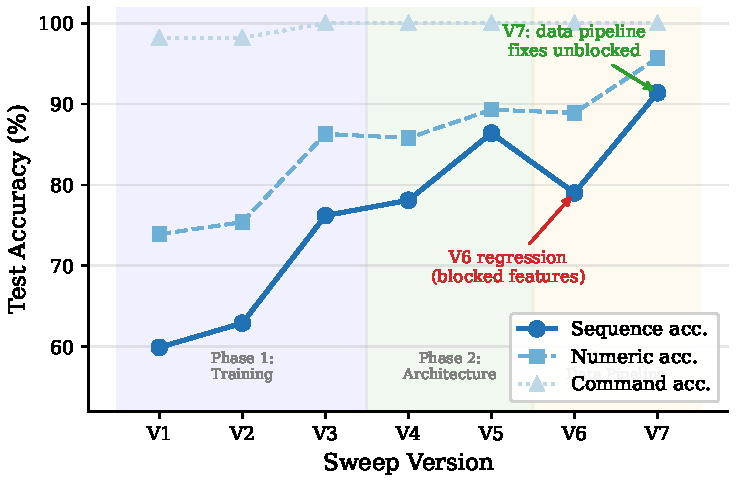
\includegraphics[width=\textwidth]{figures/sweep_progression.pdf}
\caption{Sweep progression across V1--V7. Three phases are visible: training sufficiency (V1--V3), architectural improvements via temporal context (V3--V5), and data pipeline correctness (V5--V7). V6 regressed due to blocked data features; V7 recovered and set a new best.}
\label{fig:sweep_progression}
\end{figure}

The progression (Figure~\ref{fig:sweep_progression}) reveals three distinct phases: training sufficiency (V1$\to$V3, +16.3~pp), temporal context (V3$\to$V5, +10.2~pp via MWC and memory positional encoding), and data pipeline correctness (V5$\to$V7, +5.0~pp best, +36~pp median). The detailed per-sweep narrative is in Appendix~\ref{sec:appendix_sweep}. V6 regressed to 79.0\% because three high-impact data features were structurally blocked by missing metadata in preprocessed files: window position fell back to zero-vectors, MWC used random (post-shuffle) neighbors instead of file-local windows, and non-stratified splits left 44 G-code sequences absent from certain folds' training sets. V7 re-processed data from raw CSVs, unblocking all three. The result is the largest improvement in \emph{robustness}: the median sequence accuracy rose from 33\% (V5) and 48\% (V6) to 84\% (V7), meaning that nearly every hyperparameter configuration now produces a viable model. This episode demonstrates that data pipeline correctness can dominate architectural improvements.

\subsection{Sensor Modality Importance (RQ3)}
\label{sec:rq2_modality}

Having established the baseline accuracy and the dominance of data pipeline features, we turn to the question of which sensor modalities are essential for reconstruction.

\subsubsection{Modality Ablation}
\label{sec:modality_ablation}

To determine which sensor modalities are essential for reconstruction, we retrain the full pipeline (encoder + decoder) nine times, each time excluding one modality while keeping all others. Table~\ref{tab:modality} reports the results.

\begin{table}[htbp]
\centering
\caption{Sensor Modality Ablation: Effect of Removing One Modality}
\label{tab:modality}
\small
\begin{tabular}{@{}llcccc@{}}
\toprule
\textbf{Removed} & \textbf{$F$} & \textbf{Seq.\ (\%)} & \textbf{$\Delta$} & \textbf{Class.\ Rank} \\
\midrule
None (base, f110) & 110 & $86.1 \pm 8.4$ & --- & --- \\
\midrule
Gyroscope$^\dagger$    & 92  & $58.4 \pm 34.5$ & $-$27.7 & \#6 \\
Color (RGBA) & 86  & $58.9 \pm 8.7$  & $-$27.2 & \#5 \\
Accelerometer$^\dagger$ & 92 & $63.1 \pm 35.8$ & $-$23.0 & \#7 \\
Magnetometer & 92  & $68.7 \pm 13.0$ & $-$17.4 & \#4 \\
Electrical   & 102 & $70.9 \pm 8.5$  & $-$15.2 & \#8 \\
Pressure     & 104 & $72.1 \pm 9.6$  & $-$14.0 & \#1 \\
Temperature  & 104 & $73.3 \pm 7.9$  & $-$12.8 & \#9 \\
Proximity    & 104 & $73.5 \pm 5.8$  & $-$12.7 & \#3 \\
RMS Audio    & 104 & $79.6 \pm 12.6$ & $-$6.5  & \#2 \\
\bottomrule
\multicolumn{5}{@{}l}{\scriptsize $F$ = remaining features. Class.\ Rank = ranking by ANOVA}\\
\multicolumn{5}{@{}l}{\scriptsize $F$-statistic for 9-class operation classification~\cite{encoder_paper}.}\\
\multicolumn{5}{@{}l}{\scriptsize $^\dagger$High std from Fold~5 failure (0\%); median: gyroscope 66.4\%, accelerometer 76.1\%.}
\end{tabular}
\normalsize
\end{table}

Reconstruction and classification rank sensor modalities differently (Table~\ref{tab:modality}; Spearman $\rho = -0.35$, $p = 0.36$, $n = 9$---a weak negative correlation that does not reach significance but indicates the two rankings diverge in direction). Three findings stand out:

\begin{enumerate}[leftmargin=*]
    \item \textbf{Inertial sensors dominate reconstruction.} Gyroscope ($-$27.7~pp) and accelerometer ($-$23.0~pp) together account for over 50~pp of reconstruction accuracy (Figures~\ref{fig:modality_heatmap} and~\ref{fig:fold_modality}). The high standard deviations ($\pm$34--36\%) reflect complete failure on Fold~5 (0\% sequence accuracy) when either is removed, indicating that inertial signals are essential for the window-position-to-G-code mapping on certain file configurations.
    \item \textbf{Color is unexpectedly critical ($-$27.2~pp).} The APDS-9960 RGBA sensor, ranked \#5 for classification, is the second most important modality for reconstruction. The mechanism by which removing four low-bandwidth color channels drops reconstruction accuracy by 27~pp is not obvious, and an explicit correlation test (detailed below) ruled out the most natural hypothesis.
    \item \textbf{Audio is the least important for reconstruction ($-$6.5~pp)} despite being the second-strongest classifier feature by ANOVA. Audio's high classification $F$-statistic reflects its ability to distinguish operation \emph{types} (cutting vs.\ air-cutting), but within an operation type, acoustic signatures carry little coordinate-level information.
\end{enumerate}

The reversal between classification and reconstruction importance has direct implications for sensor selection in deployment. A rig optimized for operation monitoring (classification) would prioritize pressure and audio; a rig optimized for G-code verification (reconstruction) would prioritize gyroscope, color, and accelerometer. A minimal three-modality reconstruction rig (gyroscope + color + accelerometer, 60 channels) would retain the three largest contributors, though the interaction effects of simultaneous removal remain untested.

\paragraph{The color-hypothesis test.} One natural explanation for the color channel's reconstruction importance is that ambient light at the sensor boards varies with the table's Y-coordinate---e.g., because lateral motion changes proximity to the enclosure walls or to fixed illumination sources---providing a direct spatial signal that the decoder exploits for Y-axis disambiguation. To test this, we computed Pearson and Spearman correlations between each of the 24 raw color channels (4 color components $\times$ 6 sensor boards) and the machine-reported Y-coordinate (\texttt{posy}), both pooled across all 120 aligned files and within-file to remove between-file setup drift. Pooled correlations are all in the range $|r| < 0.12$. The highest within-file mean $|r|$ is 0.122 (frame\_l3 board, Red channel); the lowest is 0.052 (spindle2, Blue). By the conventional interpretation of correlation strength, none of the color channels meaningfully tracks the Y-coordinate. We therefore reject the ambient-light-gradient hypothesis. The mechanism by which the color sensor contributes 27~pp to reconstruction accuracy remains unexplained. Candidate hypotheses include (a) correlation with operation-class-specific temporal patterns that the encoder's cross-modal attention amplifies, (b) electromagnetic or thermal cross-talk between the APDS-9960 and the IMU on the same board, and (c) some artifact of the robust scaler's interaction with the low-variance color signal. We leave identification of the true mechanism to future work.

\begin{figure}[htbp]
\centering
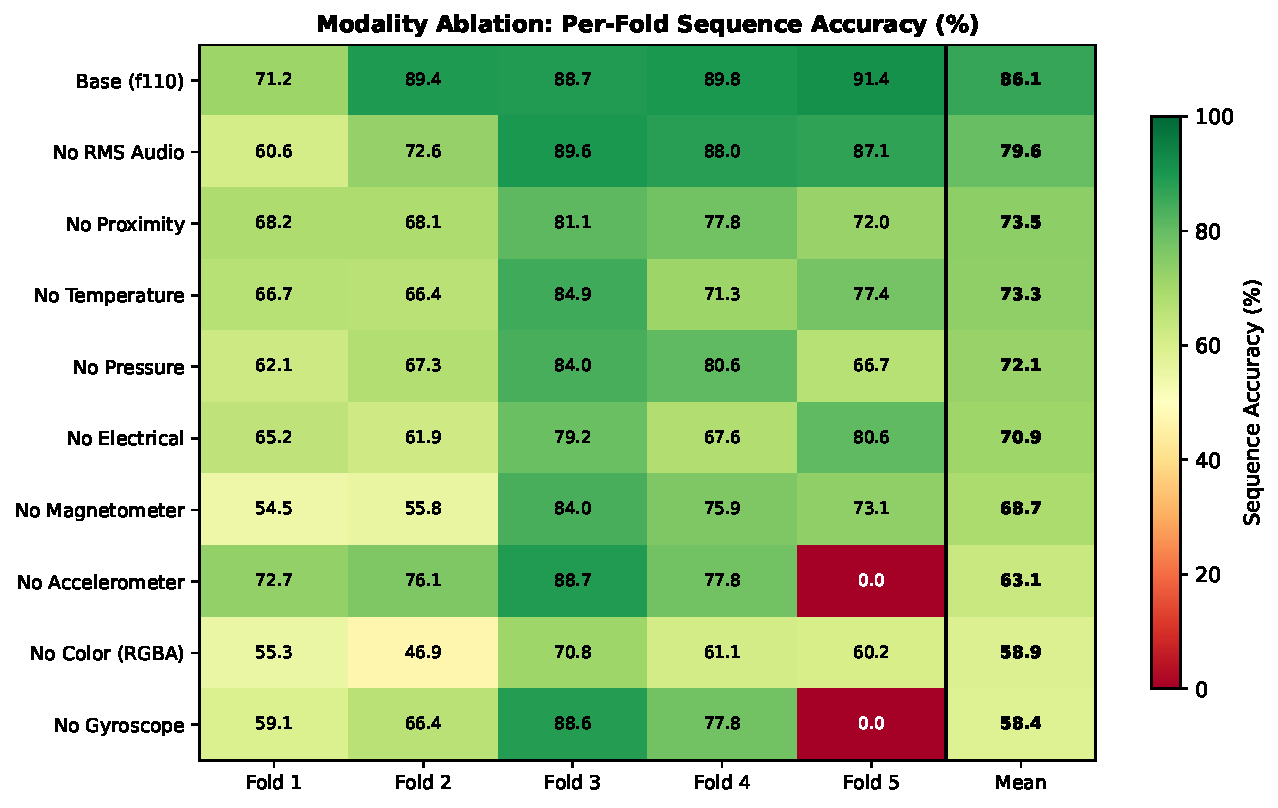
\includegraphics[width=\textwidth]{figures/modality_ablation_heatmap.pdf}
\caption{Per-fold sequence accuracy for each modality removal. Gyroscope and accelerometer removal causes catastrophic failure on Fold~5 (0\%), while other folds remain viable. Color removal uniformly degrades all folds. Audio removal has the smallest effect across all folds.}
\label{fig:modality_heatmap}
\end{figure}

\subsubsection{Encoder Configuration: Confound-Free Reconstruction}

The encoder configuration ablation (Table~\ref{tab:encoder_ablations}) addresses a critical validity concern: the encoder paper~\cite{encoder_paper} identified proximity and pressure channels as barometric confounds (ANOVA $F > 2000$), raising the question of whether reconstruction accuracy is inflated by these non-machining signals.

\begin{table}[htbp]
\centering
\caption{Encoder Feature Configuration: Confound-Free Reconstruction. The f98 encoder excludes proximity and pressure channels identified as barometric confounds in~\cite{encoder_paper}.}
\label{tab:encoder_ablations}
\small
\begin{tabular}{@{}lcccc@{}}
\toprule
\textbf{Config} & \textbf{$F$} & \textbf{Enc.\ Class.} & \textbf{Seq.\ Acc.} & \textbf{$\Delta$} \\
\midrule
f110 (full)              & 110 & $92.9\%$ & $86.0 \pm 7.2$ & --- \\
f98 (no prox/pres)       & 98  & $92.4\%$ & $81.1 \pm 9.5$ & $-$4.9 \\
f98 (optimized encoder)  & 98  & $94.8\%$ & $82.5 \pm 9.7$ & $-$3.5 \\
\bottomrule
\multicolumn{5}{@{}l}{\scriptsize $F$ = number of sensor features. Enc.\ Class.\ = encoder 9-class}\\
\multicolumn{5}{@{}l}{\scriptsize classification accuracy. f98 excludes proximity and pressure}\\
\multicolumn{5}{@{}l}{\scriptsize channels identified as barometric confounds in~\cite{encoder_paper}.}
\end{tabular}
\normalsize
\end{table}

The confound-free f98 encoder (no proximity or pressure) achieves 81.1\% mean sequence accuracy---a 4.9~pp drop from the f110 ablation base of 86.0\%. Optimizing the f98 encoder's hyperparameters (yielding 94.8\% classification accuracy, \emph{higher} than f110's 92.9\%) recovers only 1.4~pp to 82.5\%. This reveals two important findings:

\begin{enumerate}[leftmargin=*]
    \item \textbf{Confound-free reconstruction is viable.} 82.5\% sequence accuracy without proximity/pressure channels confirms that the core sensor modalities (accelerometer, gyroscope, temperature, audio, electrical) carry sufficient information for G-code reconstruction.
    \item \textbf{Better classification $\neq$ better reconstruction.} The f98 optimized encoder achieves 1.9~pp \emph{higher} classification accuracy than f110 but 3.5~pp \emph{lower} reconstruction accuracy. The proximity/pressure channels carry real signal for coordinate-level discrimination that is not captured by the 9-class classification metric.
\end{enumerate}

\subsection{Minimum Viable Configuration (RQ4)}
\label{sec:rq4_minimum}

For deployment in real manufacturing environments, the full 110-feature, 64-second, 22.1M-parameter configuration may be impractical. This subsection examines how much can be reduced while maintaining viable reconstruction.

\subsubsection{Observation Window Size}
\label{sec:window_ablation}

Table~\ref{tab:window} reports reconstruction accuracy as a function of the observation window duration.

\begin{table}[htbp]
\centering
\caption{Window Size Ablation. Halving the window from 64~s to 32~s costs 9.2~pp but doubles temporal resolution.}
\label{tab:window}
\small
\begin{tabular}{@{}cccccc@{}}
\toprule
\textbf{Window} & \textbf{Duration} & \textbf{Windows} & \textbf{Seq.\ (\%)} & \textbf{$\Delta$} \\
\midrule
$W{=}256$ & 64~s  & 545   & $86.1 \pm 8.4$  & --- \\
$W{=}128$ & 32~s  & 861   & $76.9 \pm 5.4$  & $-$9.2 \\
$W{=}64$  & 16~s  & 1{,}964 & $70.6 \pm 5.0$  & $-$15.5 \\
\bottomrule
\end{tabular}
\normalsize
\end{table}

Halving the window from 256 to 128 timesteps (64~s to 32~s) reduces sequence accuracy by 9.2~pp but increases temporal resolution 1.6$\times$ (861 vs.\ 545 evaluation points per dataset). Quartering to 64 timesteps (16~s) costs 15.5~pp but provides 3.6$\times$ more evaluation points. The 76.9\% accuracy at 32~s may be sufficient for structural-level monitoring (command detection remains above 95\%), while the full 64~s window is needed for numeric-level coordinate reconstruction.

The accuracy drop is consistent with the encoder bottleneck hypothesis: shorter windows contain less discriminative information for the frozen encoder to compress, reducing the quality of the memory representation that the decoder attends to. Notably, the fold variance decreases with shorter windows ($\pm$8.4 at $W{=}256$ vs.\ $\pm$5.0 at $W{=}64$), suggesting that the hardest fold's difficulty is driven by long-range temporal patterns that shorter windows cannot capture.

\subsubsection{Decoder Capacity}

Capacity is not the bottleneck. The ablations in Table~\ref{tab:ablations} (conditions 2C1--2C3) confirm that the decoder is overparameterized for this task once data handling is correct. A 2-layer decoder with $d_\text{model} = 192$ and 4 attention heads achieves 84.4\%, only 1.6~pp below the full 8-layer, $d{=}384$, 12-head architecture. This minimal decoder has approximately 3.0M parameters---a 7.4$\times$ reduction from the full 22.1M-parameter architecture---making it feasible for edge deployment on embedded hardware alongside the CNC controller.

\subsubsection{Deployment Implications}

Combining the results above, a minimum viable reconstruction system could use: (1)~the confound-free f98 encoder (82.5\%), (2)~a 32-second observation window (76.9\% at full encoder, trading accuracy for 1.6$\times$ temporal resolution), and (3)~a 3.0M-parameter decoder (84.4\% at full window). These reductions are not independently validated in combination, so interaction effects may further degrade accuracy. However, the structural reconstruction (command + parameter accuracy $>$95\%) remains viable across all reduced configurations, suggesting that a lightweight deployment could reliably detect command-level anomalies (wrong operation type, unexpected parameter) even if coordinate-level precision is reduced.

\begin{figure}[htbp]
\centering
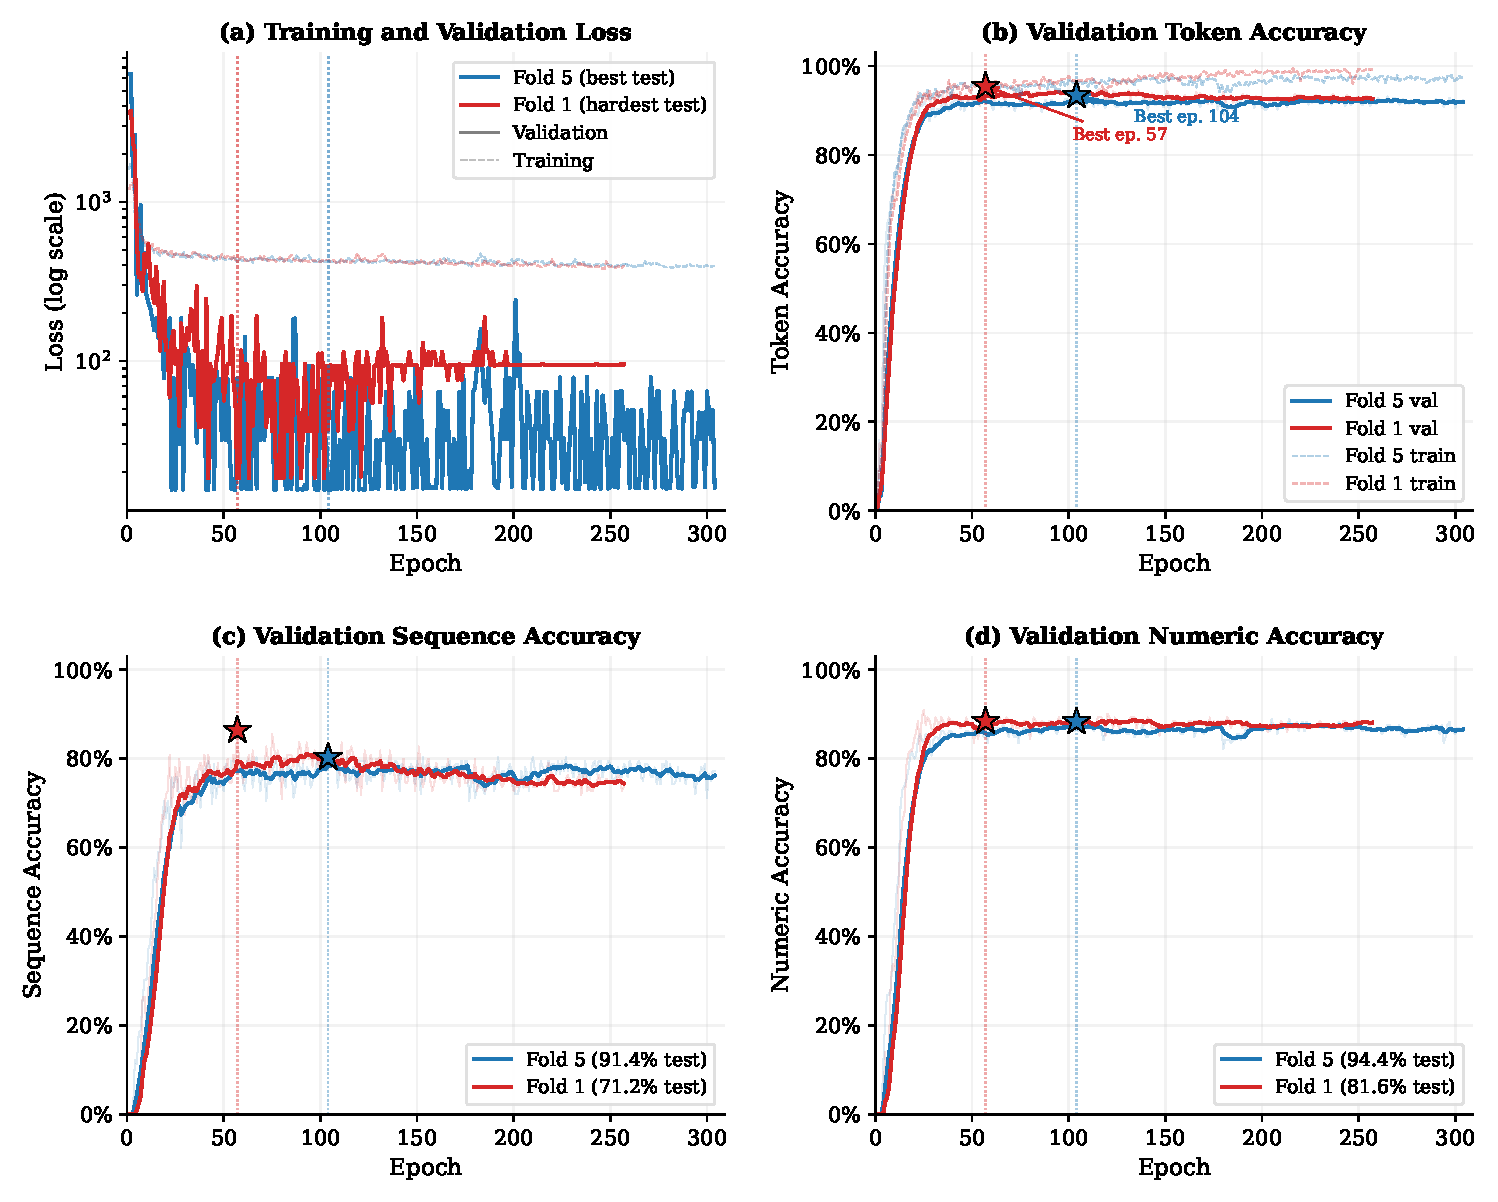
\includegraphics[width=\textwidth]{figures/training_curves.pdf}
\caption{Validation accuracy over training for the best V7 trial (Fold~5, test sequence accuracy 91.4\%). Token and numeric accuracy plateau after $\sim$200 epochs, while sequence accuracy continues to improve slowly through 500 epochs, consistent with the finding that structural prediction converges early while numeric prediction requires longer training.}
\label{fig:training_curves}
\end{figure}

Figure~\ref{fig:training_curves} shows the training dynamics of the best V7 trial. Token-level accuracy converges rapidly ($\sim$200 epochs) because structural tokens (commands, parameters) are predicted with high confidence early. Sequence-level accuracy lags because it requires \emph{all} tokens---including the numerically ambiguous ones---to be correct simultaneously. The digit weight $w_d$, which controls the relative importance of numeric versus structural loss, shows no significant effect in V7: all three tested values ($w_d \in \{15, 20, 30\}$) achieve the same best accuracy (91.4\%) with similar means (81.2\%, 81.3\%, 82.1\% respectively), suggesting that the preprocessing corrections reduced the difficulty of numeric prediction to the point where the loss weighting no longer matters.


\begin{figure}[htbp]
\centering
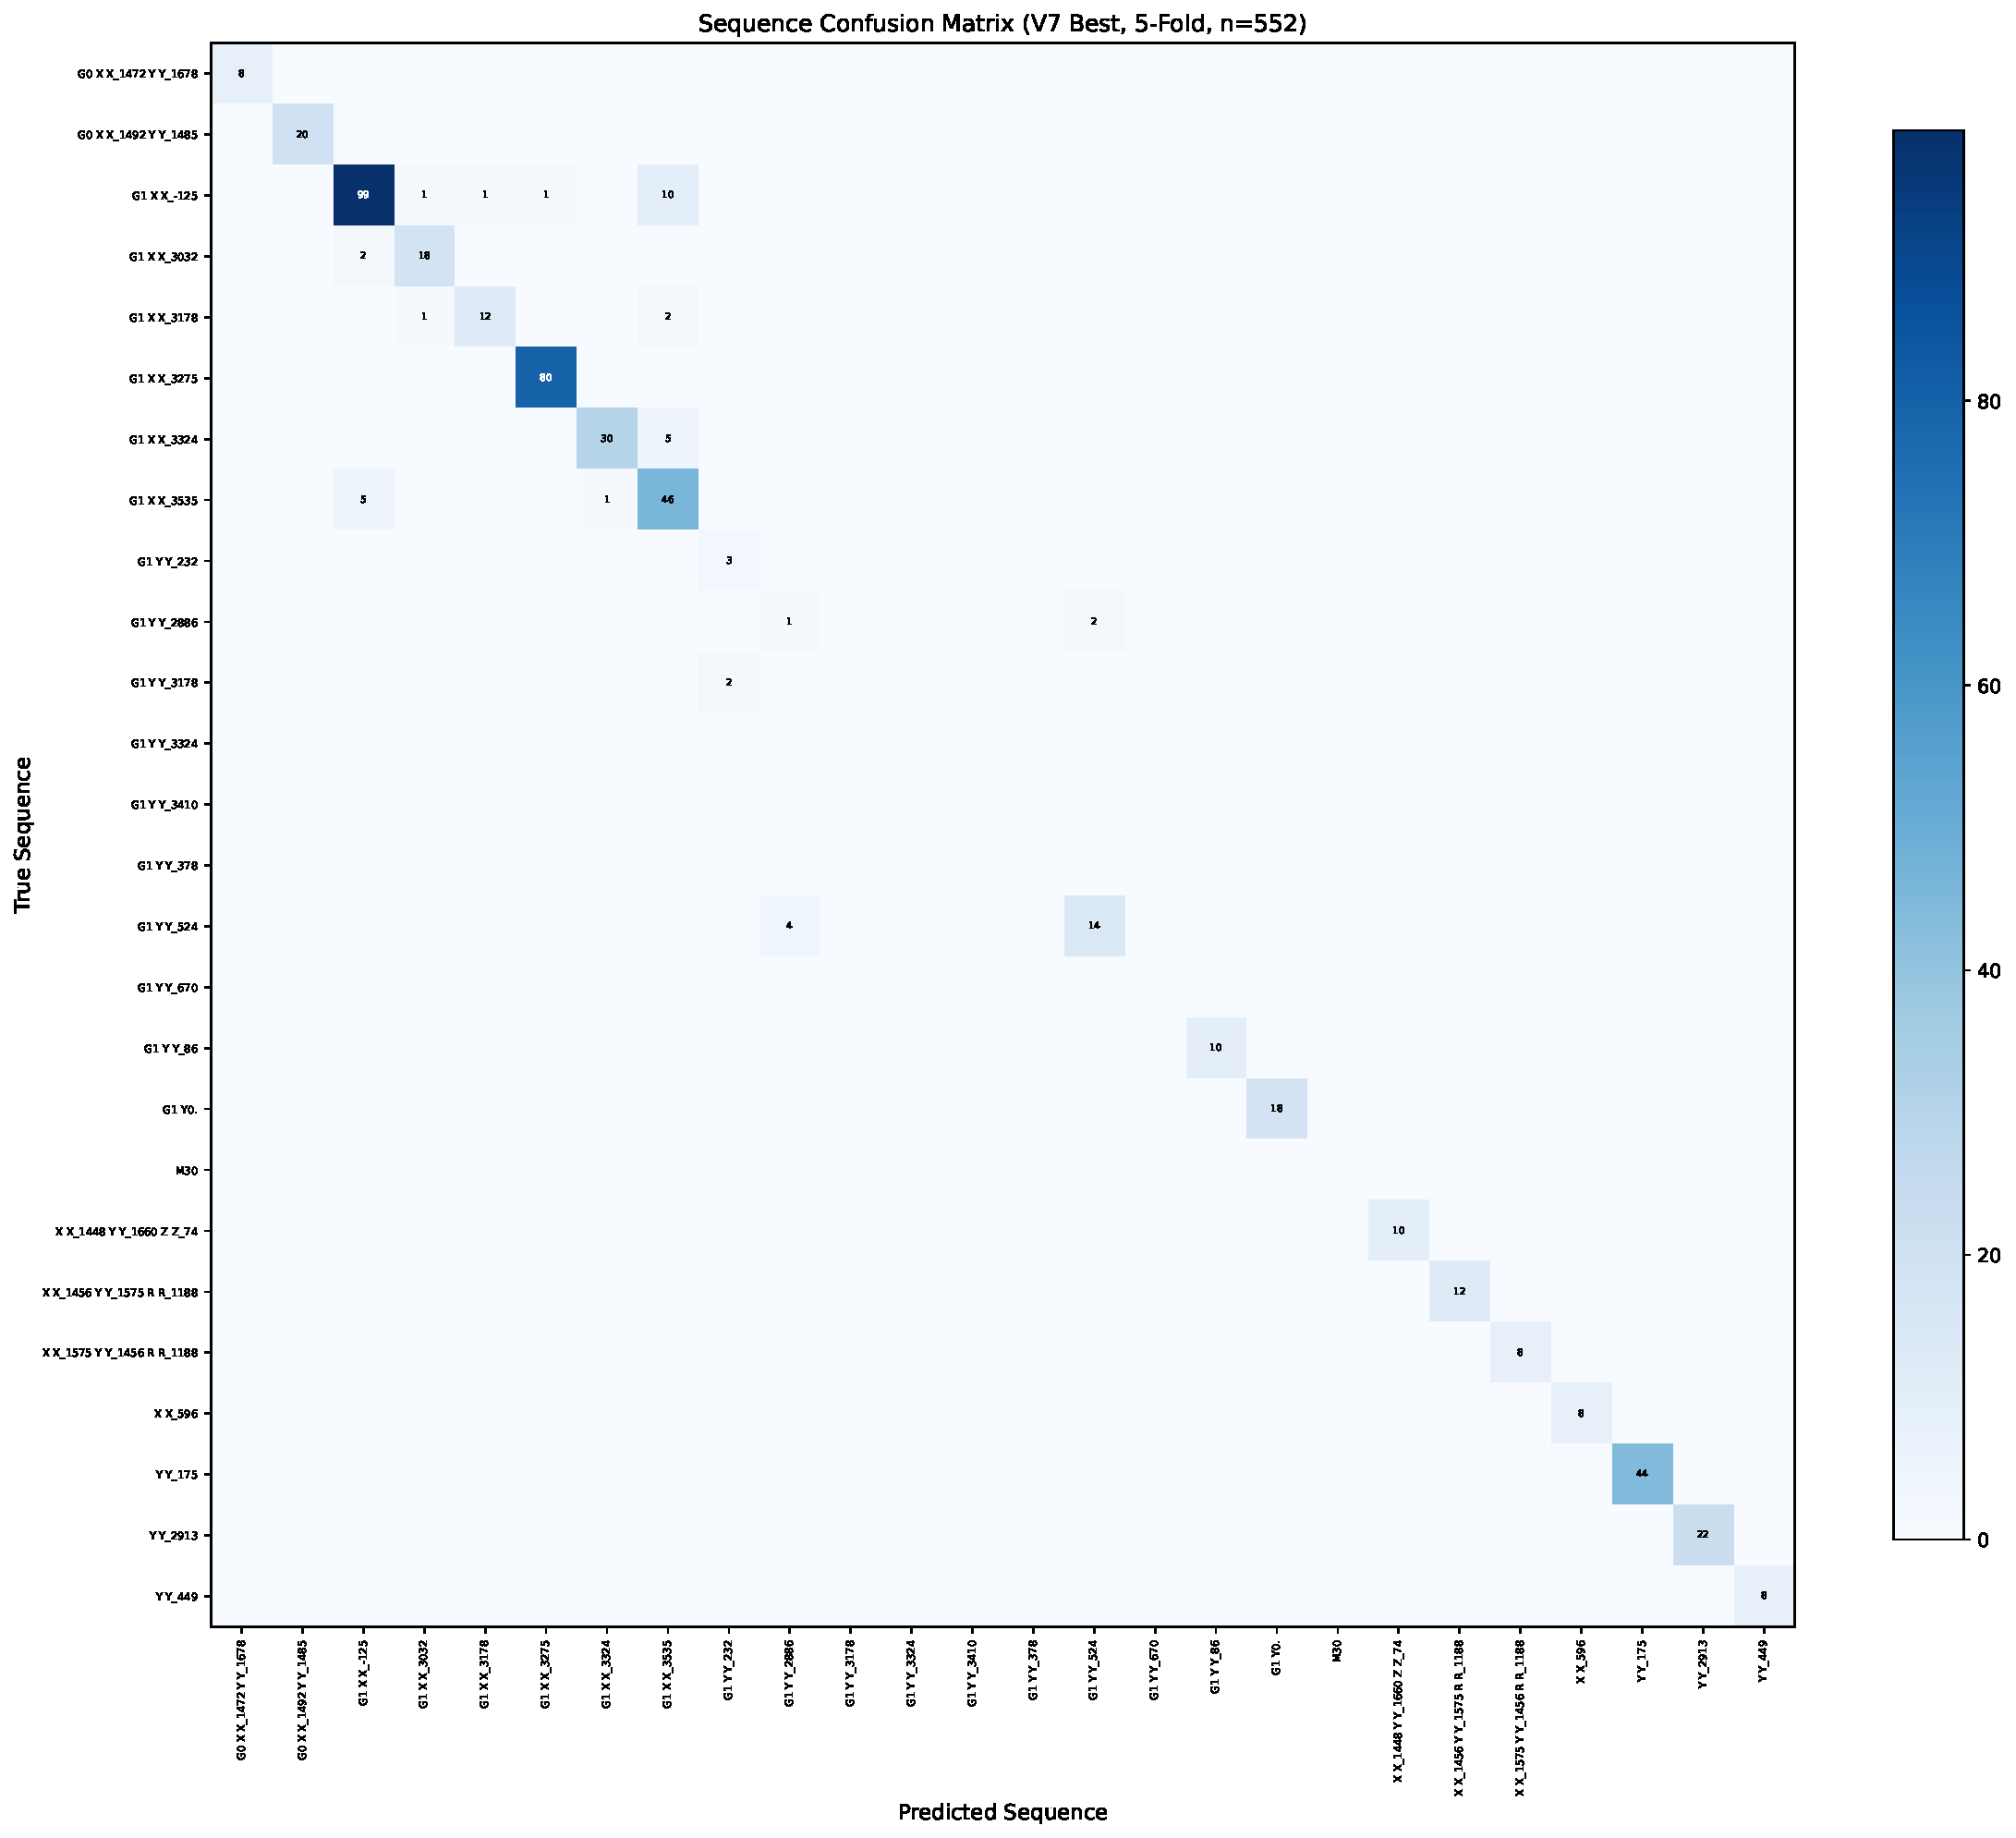
\includegraphics[width=\textwidth]{figures/confusion_matrix_v7.pdf}
\caption{Sequence-level confusion matrix across all 552 test windows (V7 best config, 5 folds, teacher-forced decoding). The dominant off-diagonal pattern is Y-axis step-over confusion: sequences differing only in $Y{=}0.175 \leftrightarrow Y{=}2.913 \leftrightarrow Y{=}0.449$. Face milling and adaptive clearing under air-cutting achieve 100\% sequence accuracy. Cross-class confusion is rare; most errors are within-class numeric substitutions in the active-cutting and damaged-spindle conditions.}
\label{fig:confusion}
\end{figure}

\subsection{Generalization to Unseen Toolpath Classes}
\label{sec:ood}

The cross-validation in Section~\ref{sec:rq1_accuracy} is \emph{in-distribution}: every fold's training set contains files from all three toolpath classes (adaptive, face, pocket), because the stratified round-robin split preserves class balance within each fold. Under those conditions a position-based lookup table reaches 90.4\% (Table~\ref{tab:baselines}) without any model, because (source\_file, window\_index) is nearly a unique key for the G-code sequence on this fixed-geometry dataset. This leaves open the question of whether the decoder learns anything that a lookup table cannot---and, more scientifically, whether sensor-to-G-code reconstruction transfers at all when the target toolpath class has been withheld from training.

To test this, we construct three leave-one-toolpath-out splits. For each held-out toolpath class $c \in \{\text{adaptive},\ \text{face},\ \text{pocket}\}$ we train the full V7 decoder (reusing the V7 frozen encoder checkpoint) on all files from the two non-heldout toolpath classes, with a stratified 80/20 train/val split, and evaluate on every window from the held-out class. Split sizes are: heldout-adaptive 333/84/128; heldout-face 240/61/244; heldout-pocket 297/75/173 train/val/test windows. The encoder reuses the fold-1 checkpoint; this is a conservative bias because the encoder was originally trained in the 5-fold CV setting and saw some windows from every toolpath---any transfer failure under this setup is a real decoder-level limit, not an encoder-level one.

For the lookup-table baseline on the same splits, the majority map from (window\_index, total\_windows) is built on the non-heldout train$\cup$val pool and applied to the heldout test pool.

\begin{table}[htbp]
\centering
\caption{Held-Out-Toolpath Generalization (\%). Each row is a single-seed run; val reflects performance on the non-heldout distribution, test reflects the held-out toolpath. Both methods produce 0\% exact-sequence accuracy on test because held-out toolpaths use numeric coordinate values the model has never seen. The decoder preserves command and parameter-type accuracy at levels substantially above the lookup table across all three splits.}
\label{tab:ood}
\small
\begin{tabular}{@{}llcccccc@{}}
\toprule
\textbf{Heldout} & \textbf{Method} & \textbf{Split} & \textbf{Seq} & \textbf{Tok} & \textbf{Cmd} & \textbf{Param} & \textbf{Num} \\
\midrule
\multirow{3}{*}{adaptive}
& Decoder & val  & 81.0 & 94.7 & 100.0 & 96.4 & 88.0 \\
& Decoder & test & 0.0  & 16.4 & 0.0   & 55.1 & 0.0 \\
& Lookup  & test & 0.0  & 0.0  & 0.0   & 0.0  & 0.0 \\
\midrule
\multirow{3}{*}{face}
& Decoder & val  & 86.9 & 95.6 & 100.0 & 94.6 & 91.9 \\
& Decoder & test & 0.0  & 49.3 & 78.3  & 82.6 & 0.0 \\
& Lookup  & test & 0.0  & 2.5  & 4.9   & 2.5  & 0.0 \\
\midrule
\multirow{3}{*}{pocket}
& Decoder & val  & 92.0 & 97.7 & 100.0 & 98.3 & 95.4 \\
& Decoder & test & 0.0  & 50.1 & 89.5  & 59.5 & 0.0 \\
& Lookup  & test & 0.0  & 36.4 & 80.2  & 33.5 & 0.0 \\
\bottomrule
\end{tabular}
\normalsize
\end{table}

Three findings (Table~\ref{tab:ood}) deserve attention.

\textbf{Both methods collapse on sequence accuracy.} Neither the decoder nor the lookup table recovers a single exact G-code sequence on any held-out split. This is not a bug. It is the predicted consequence of the physics-ceiling analysis in Sections~\ref{sec:rq3_pipeline} and~\ref{sec:y_ambiguity}: the numeric coordinate values used by the held-out toolpath class are not present in the training vocabulary at all (the 712-token vocabulary is geometry-specific, and each toolpath class generates a disjoint subset of numeric tokens). Exact-sequence reconstruction therefore requires that at least one instance of each target sequence have been seen during training. Neither a lookup table nor the current decoder can violate this constraint.

\textbf{Numeric accuracy collapses to zero for the same reason.} The numeric coordinate tokens for the held-out toolpath are never seen during training and thus cannot be predicted by any method that treats coordinates as a closed vocabulary. The digit-by-digit open-vocabulary framework of~\cite{grammar_paper} is a natural remedy and is identified as future work (Section~\ref{sec:discussion}).

\textbf{Command and parameter-type accuracy, however, transfer substantially---and the decoder transfers them much better than the lookup table.} On heldout-face, the decoder reaches 78.3\% command accuracy and 82.6\% parameter-type accuracy; the lookup table reaches 4.9\% and 2.5\%. On heldout-pocket, the decoder reaches 89.5\%/59.5\%; the lookup reaches 80.2\%/33.5\%. Even on heldout-adaptive---the hardest split, because adaptive clearing uses distinctive trochoidal arc commands (G2/G3) that face and pocket do not---the decoder preserves 55.1\% parameter-type accuracy, against 0.0\% for the lookup. Averaged across the three splits, the decoder's parameter-type accuracy advantage over the lookup table is 53.1~pp, and its command accuracy advantage is 27.3~pp. These gaps measure what the autoregressive grammar decomposition learns that a positional lookup cannot: the toolpath-invariant structure of G-code (motion-command dynamics, parameter-letter regularities) rather than just the toolpath-specific mapping from position to sequence.

\textbf{On heldout-adaptive the decoder collapses to 0\% command accuracy.} Face and pocket toolpaths primarily use G0 and G1 motion commands; adaptive clearing additionally uses G2/G3 arcs for trochoidal retract moves. A decoder that has never seen G2/G3 during training cannot emit them, and the grammar constraints (which forbid BOS$\to$G2/G3 when those tokens are absent from the training distribution) lock the decoder to a small set of tokens it has learned. This is a clean falsification of any claim that the decoder would generalize to genuinely novel command tokens on this dataset, and it sharpens the scope of what held-out-toolpath transfer actually means: \emph{structural} transfer (parameter letters, modal-persistence grammar) is real, but transfer to genuinely unseen motion-command tokens is not.

The overall message of the held-out-toolpath experiment is narrower and more honest than ``the decoder generalizes.'' On a fixed-geometry benchmark where positional metadata is nearly deterministic, neither a decoder nor a lookup can produce novel exact G-code sequences. What differs between them is how much of G-code's universal grammar---motion commands and parameter letters that mean the same thing in every toolpath---is preserved under distribution shift. The decoder preserves substantially more; the lookup preserves essentially none. This is the advantage that sensor-conditioned reconstruction brings, and it is the advantage one would expect to matter in anomaly-detection applications where the signal of interest is a structural deviation from expected grammar (command substitution, parameter swap) rather than a coordinate-level mismatch.

\paragraph{Limitations of this experiment.} The three splits are single-seed runs, not multi-seed retrains; seed variance at the structural level is unknown. The reused fold-1 encoder has seen some windows from every toolpath (through its 5-fold CV training), so the reported numbers slightly overstate what a fully held-out pipeline would achieve---we believe this slight optimism is acceptable because both methods are compared against the same biased encoder and because the decoder's transfer advantage over the lookup table comes from the decoder itself, not the encoder. Finally, the three held-out splits differ in training-set size (240--333 windows), which confounds toolpath-specific difficulty with training-set-size effects; a full balanced held-out evaluation would require additional experiments.

\subsection{Numeric Error Granularity}
\label{sec:y_ambiguity}

Not all sequence errors are equal. When the decoder predicts an incorrect sequence, the error is typically localized: the command and parameter tokens are correct, and only one or two numeric digit tokens differ. The most common error pattern is a single-digit substitution in the Y-axis value (e.g., predicting the digit sequence for $Y = 0.1755$ instead of $Y = 2.9132$), which changes the meaning of the coordinate but leaves the rest of the G-code line intact. Errors that span multiple token positions (e.g., predicting \texttt{G2} when the target is \texttt{G1 X... Y...}) are rare, consistent with the 98.1\% mean command accuracy.

The sequence-level confusion matrix (Figure~\ref{fig:confusion}) and per-head confusion matrices (Figure~\ref{fig:per_head}) confirm this pattern. The command and parameter heads are near-diagonal (few off-diagonal entries), while the Y-axis numeric head shows the characteristic step-over confusion pattern. This error structure has implications for anomaly detection: even when the decoder makes a reconstruction error, the \emph{type} of error (Y-axis step-over confusion) is predictable and can be distinguished from the error patterns that a genuine attack would produce (e.g., command substitution, feed rate manipulation, or coordinate shifts along unexpected axes).


\begin{figure}[H]
\centering
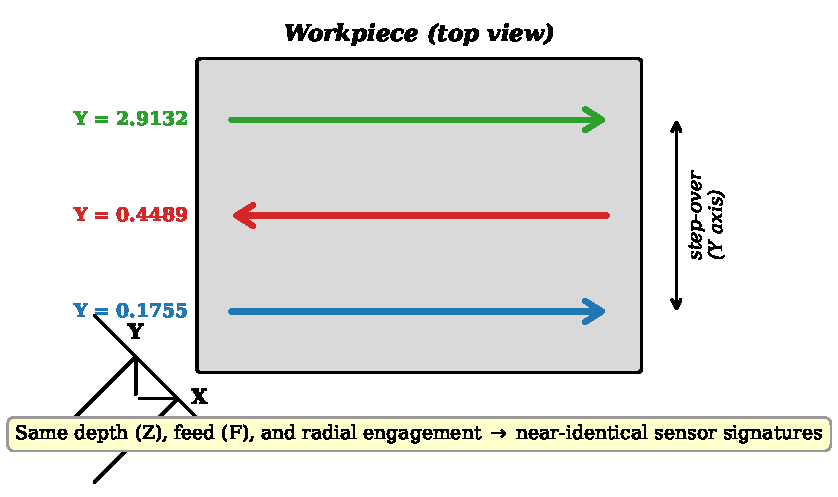
\includegraphics[width=0.75\textwidth]{figures/stepover_diagram.pdf}
\caption{Lateral step-over passes at different Y~coordinates. Each pass follows the same trajectory in the XZ~plane with identical cutting conditions (depth, feed rate, radial engagement), producing sensor readings that are indistinguishable within a single observation window. Full-precision Y~values shown.}
\label{fig:stepover}
\end{figure}

The Y-axis values 0.1755, 2.9132, and 0.449 correspond to successive lateral step-over positions: each pass follows a similar trajectory in the XZ~plane at a different Y~coordinate. In 3-axis vertical milling, the cutting dynamics---forces, accelerations, acoustic emission---are governed primarily by the depth of cut~(Z), feed rate~(F), and radial engagement, not the absolute lateral position. Consequently, passes at different Y~step-over positions produce sensor readings that are indistinguishable within a single observation window. At 0.635~mm depth in UHMW-PE, the step-over distance of 3.81~mm produces no measurable change in cutting force, vibration amplitude, or acoustic emission---the tool engagement geometry is identical at each Y~coordinate.

Figure~\ref{fig:stepover} illustrates this geometry. Within a 256-timestep window, the sensor measurements during a pass at $Y = 0.1755$ and a pass at $Y = 2.9132$ are statistically indistinguishable. The physical cutting conditions are identical; only the table's lateral position differs. The Y-value confusion matrix (Figure~\ref{fig:y_confusion}) confirms this pattern: the dominant off-diagonal entries correspond to Y-value pairs at nearby step-over positions. The window position feature (V7) directly addresses this by providing the decoder with the window's ordinal position within the file, which is strongly correlated with step-over pass number. The effect is dramatic: Fold~5 jumped from 52.7\% (V6, no window position) to 91.4\% (V7, with window position)---a 38.7-point improvement attributable primarily to Y-axis disambiguation.

The preceding sections quantified overall accuracy and identified which features and modalities matter most. This section examines where the decoder fails and why.

% ============================================================================
\section{Error Analysis}
\label{sec:errors}

\subsection{Error Decomposition}

At 86.1\% mean cross-fold sequence accuracy (91.4\% best fold), the remaining errors decompose hierarchically:

\begin{itemize}[leftmargin=*]
    \item \textbf{Command errors: $<$2\%.} Command accuracy averages 98.1\% across folds, with two folds at 100\%. The decoder rarely confuses motion types (G0/G1/G2/G3), as confirmed by the token-type confusion matrix (Figure~\ref{fig:token_type_confusion}).
    \item \textbf{Parameter type errors: $<$1\%.} Parameter addresses (X, Y, Z, F, R) average 97.6\% accuracy across folds.
    \item \textbf{Numeric value errors: $\sim$8.7\%.} The dominant error source. Nearly all numeric errors involve:
    \begin{itemize}[]
        \item Y-axis step-over confusion: $0.1755 \leftrightarrow 2.9132 \leftrightarrow 0.449$ (lateral passes with identical cutting conditions)
        \item X-axis confusion: geometrically similar coordinates producing indistinguishable sensor responses
    \end{itemize}
\end{itemize}

The improvement from V5 ($75.1 \pm 10.0\%$ cross-fold mean) to V7 ($86.1 \pm 8.4\%$) was driven primarily by resolving Y-axis step-over ambiguity through window position metadata, confirming the information-theoretic analysis below.

\subsection{Decoder Representation Analysis}

To understand what the decoder learns internally, Figures~\ref{fig:decoder_pca} and~\ref{fig:decoder_tsne} visualize the decoder's hidden states via PCA and t-SNE. The token-type PCA (Figure~\ref{fig:decoder_pca}) shows clear separation between command, parameter, and numeric tokens in the decoder's representation space, confirming that the hierarchical token decomposition is reflected in the learned representations. The numeric-token t-SNE (Figure~\ref{fig:decoder_tsne}) reveals clustering by coordinate axis (X, Y, Z, R values occupy distinct regions), with within-axis structure showing that similar coordinate values are nearby in the decoder's representation. This spatial organization explains why numeric errors are typically within-axis substitutions rather than cross-axis confusions.

\begin{figure}[H]
\centering
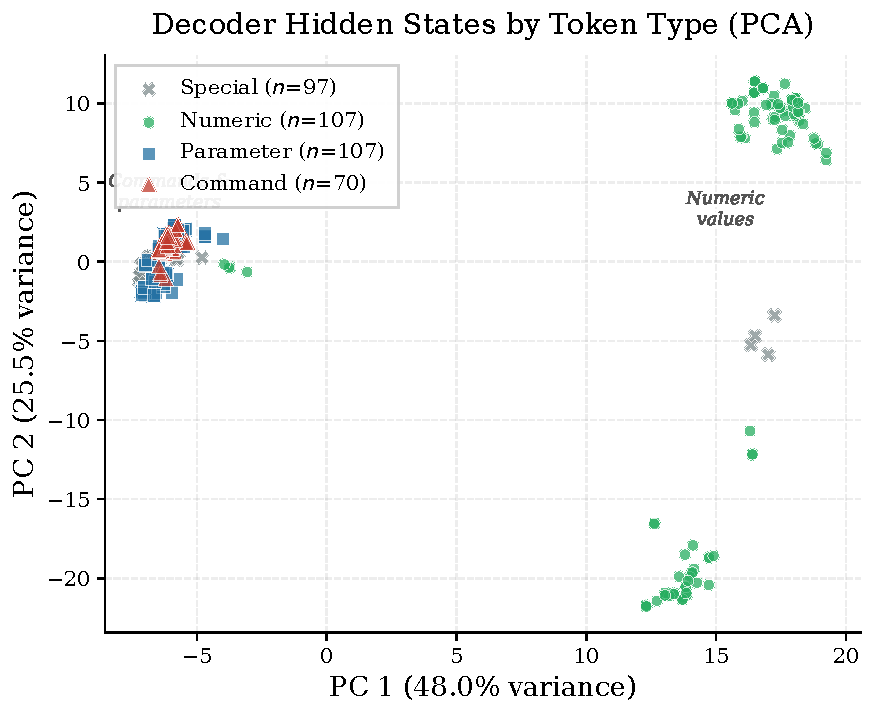
\includegraphics[width=0.75\textwidth]{figures/decoder_token_pca.pdf}
\caption{PCA of decoder hidden states by token type (Fold~5, 93 test windows). Commands, parameters, and numeric tokens occupy distinct regions, confirming that the decoder learns type-structured representations.}
\label{fig:decoder_pca}
\end{figure}

\begin{figure}[H]
\centering
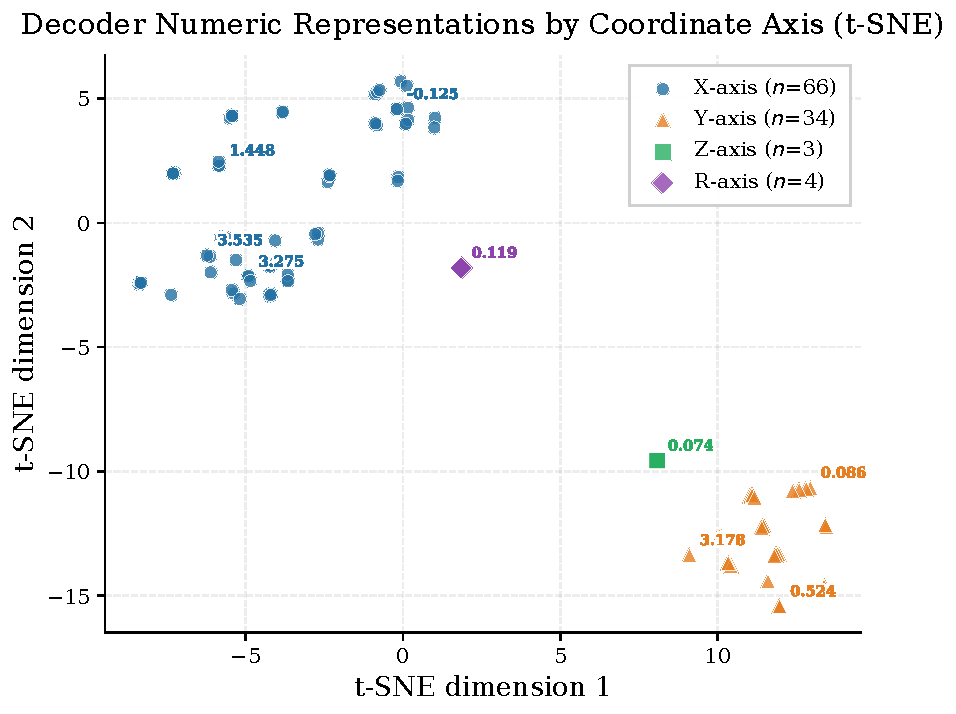
\includegraphics[width=0.75\textwidth]{figures/decoder_numeric_tsne.pdf}
\caption{t-SNE of decoder hidden states for numeric tokens only, colored by coordinate axis. X, Y, Z, and R values cluster by axis, with within-axis proximity reflecting coordinate similarity.}
\label{fig:decoder_tsne}
\end{figure}

\subsection{Per-Operation Analysis}

The per-operation breakdown (Table~\ref{tab:per_class}) reveals systematic variation in reconstruction difficulty (Figures~\ref{fig:per_class_metric} and~\ref{fig:error_type}). The damaged-pocket class (60.0\%) is the hardest overall, combining the geometric complexity of pocketing with the vibration noise from spindle damage. Fold~1 remains the hardest fold at 71.2\% sequence accuracy on its 132 test windows, suggesting that its specific file combination contains toolpaths with inherently ambiguous sensor signatures that neither temporal context nor window position can resolve.

\subsection{Information-Theoretic Analysis}

The normalized information gain of window position for Y-value prediction is $(H(Y) - H(Y|\text{pos})) / H(Y) = (3.77 - 1.59) / 3.77 = 57.8\%$, where $H$ denotes Shannon entropy in bits computed over training windows containing Y-axis coordinates ($n = 656$). This means that knowing a window's ordinal position within the file eliminates over half the uncertainty about its Y-axis value. The relationship is strongly structured:

\begin{itemize}[leftmargin=*]
    \item Window positions 0--1: $Y = 0.1755$ is the most frequent value ($\sim$35\%)
    \item Window position 2: $Y = 2.9132$ is dominant (52--93\% depending on fold)
    \item Later positions: increasingly determined by toolpath strategy and operating condition
\end{itemize}

The structural regularity makes window position the single highest-impact feature for numeric reconstruction, consistent with V7's design decision to always enable it.

The error analysis reveals a clear hierarchy: structural prediction is solved, numeric prediction is limited by sensor physics, and window position metadata resolves most of the remaining ambiguity. The following section discusses broader implications for manufacturing, deployment, and future research.

% ============================================================================
\section{Discussion}
\label{sec:discussion}

\begin{figure}[htbp]
\centering
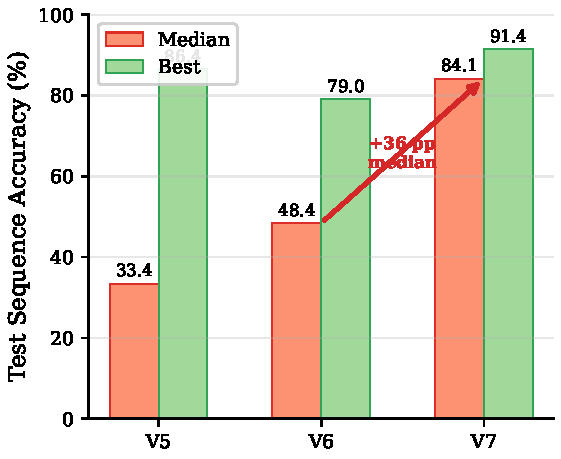
\includegraphics[width=0.75\textwidth]{figures/data_pipeline_impact.pdf}
\caption{Data pipeline impact: median vs.\ best sequence accuracy across V5--V7. The +36~pp median improvement from V6 to V7 demonstrates that data-handling correctness dominates architectural improvements.}
\label{fig:data_pipeline_impact}
\end{figure}

\subsection{Why Is Command Prediction Solved but Coordinate Prediction Not?}

Figure~\ref{fig:data_pipeline_impact} summarizes the dominance of data handling over architecture. The structural component of G-code---commands and parameter addresses---is determined by toolpath geometry. Adaptive clearing follows trochoidal paths with frequent direction reversals; face milling sweeps in linear passes with periodic step-overs; pocket machining alternates between plunges and lateral clearing. Each strategy produces distinctive acceleration profiles and trajectory envelopes that the encoder captures reliably, reaching 98.3\% command accuracy in-distribution and still preserving 78--89\% command accuracy on two of the three held-out-toolpath splits (Section~\ref{sec:ood}). This is a meaningful form of transfer: the motion-command grammar is partially toolpath-invariant.

The numeric component---coordinate values---depends on the table's absolute lateral position. In 3-axis vertical milling, the cutting dynamics (forces, vibration, acoustic emission) are governed by depth of cut, feed rate, and radial engagement, not by the table's Y-coordinate. Two passes at $Y = 0.1755$ and $Y = 2.9132$ produce sensor readings that are statistically indistinguishable within a single 64-second window. This is a physical limitation, not a modeling choice, and it has a precise quantitative signature: with window-position metadata withheld, sequence accuracy drops from 86.1\% to 62.3\%---a 23.8~pp gap that directly measures how much of a G-code line is recoverable from sensor physics alone. The remaining numeric errors (after window position is added) concentrate on Y-values within the step-over confusion radius, and on held-out toolpaths numeric accuracy collapses to zero because unseen coordinate values are not in the closed vocabulary at all.

The structural--numeric split mirrors the separation principle in~\cite{grammar_paper} and has a practical consequence for sensor-based process verification: structural anomalies (command injection, parameter substitution) are characterized at $>$97\% in-distribution accuracy, while coordinate-level tampering would be detectable only when the deviation exceeds the step-over confusion radius of 2.74~mm.

\subsection{Where Is the Accuracy Ceiling and What Sets It?}

The encoder compresses 64 seconds of 110-channel sensor data into a 256-dimensional memory. This compression preserves toolpath-discriminative features---direction changes, engagement patterns, force profiles---but discards absolute positioning information that varies only across windows, not within them. Five observations converge on the conclusion that this encoder representation, not decoder capacity or training procedure, sets the accuracy ceiling:

\begin{enumerate}[leftmargin=*]
    \item \textbf{Fold variance exceeds every architectural effect.} The fold spread (69--90\%) is larger than any architectural ablation ($-$2.1~pp for the sensor prior, the largest).
    \item \textbf{Step-over confusion is physics-limited.} Successive lateral passes produce statistically indistinguishable sensor profiles; disambiguation requires context external to the window.
    \item \textbf{External context dominates the numeric ambiguity.} Window position accounts for 23.8 of the 24.5~pp total data-feature ablation effect, with a normalized information gain of 57.8\% for Y-value disambiguation.
    \item \textbf{The decoder is not overfitting and is overparameterized.} Mean final train-val token-accuracy gap across 25 multi-seed runs is 2.5\%, and a 3.0M-parameter decoder (2~layers, $d{=}192$) achieves 84.4\%---only 1.6~pp below the full 22.1M-parameter architecture. Capacity is not the constraint.
    \item \textbf{Decoding search is not the constraint either.} Teacher-forced, greedy autoregressive, and beam-search decoding produce numerically identical aggregate accuracies; per-item predictions differ on only 7.1\% of windows (18\% on the hardest fold), and those differences are symmetric---decode modes swap which windows they get right, but the number of correct predictions is constant. Errors are representational, not search errors.
\end{enumerate}

Preliminary fine-tuning experiments (unfreezing the encoder LSTM) improved Fold~1 by only 2.3~pp, consistent with the representation being near-optimal for the available modalities and window size. Architectures that attend across multiple windows at the encoder level---rather than concatenating independently encoded memories as the current decoder does---might capture inter-pass dynamics the current single-window encoder cannot. Whether such an architecture would \emph{break} the physics ceiling or merely \emph{approach} it more efficiently is an open question: the held-out-toolpath result (Section~\ref{sec:ood}) suggests that some component of numeric reconstruction requires genuinely new modeling assumptions (e.g., open-vocabulary digit generation) rather than just a bigger architecture.

\subsection{What Might Reconstruction Enable for Physical-Layer Verification?}

\emph{We stress that the following is a characterization of what reconstruction accuracy implies in principle, not a validated anomaly-detection result.} The reconstruction framework could in principle serve as an independent physical verification channel: comparing sensor-predicted G-code against commanded G-code would reveal discrepancies from injection attacks, parameter modification, or controller compromise~\cite{sturm2014cyber,yampolskiy2018security}. The error structure from Section~\ref{sec:errors} bounds what would be detectable and what would not. Command-level injections (substituting G0 for G1, injecting G2 arcs) would be flagged in nearly all cases given 98.3\% in-distribution command accuracy and 78--89\% command accuracy even on held-out toolpaths (Section~\ref{sec:ood}). Parameter substitution (swapping X for Y addresses) is characterized at 97.2\% in-distribution parameter accuracy. Coordinate-level tampering, however, would be detectable only when the shift exceeds the Y-axis step-over confusion radius of 2.74~mm ($|2.9132 - 0.1755|$, the dominant confusion pair)---and this radius is three orders of magnitude larger than typical precision-machining tolerances ($\pm$0.025--0.050~mm). A subtle attacker could displace coordinates within this radius without detection. Sensor-based reconstruction is therefore better suited to detecting grammar-breaking attacks (novel commands, parameter swaps) than to detecting quantitative coordinate drift. End-to-end validation of these detection capabilities---synthetic command injection, parameter substitution, leave-one-class-out novelty detection, entropy-based scoring, and physical attack experiments---is the subject of a separate companion paper~\cite{anomaly_paper} and is not claimed here.

\subsection{What Does Deployment Require?}

\textbf{Sensor configuration.} The modality ablation (Table~\ref{tab:modality}) provides direct guidance. Gyroscope, color, and accelerometer are the three most critical modalities ($-$23 to $-$28~pp each when removed). Audio contributes the least ($-$6.5~pp). A minimal deployment using only IMU boards (gyroscope + accelerometer), color sensors, and electrical monitoring retains the top-4 modalities at an estimated hardware cost of $\sim$\$492~\cite{encoder_paper}, with no controller modification required.

\textbf{Observation window.} Halving from 64~s ($W{=}256$) to 32~s ($W{=}128$) costs 9.2~pp (76.9\% accuracy) but doubles temporal resolution. A 16~s window ($W{=}64$) retains 70.6\% at 4$\times$ resolution. The choice depends on whether the application prioritizes accuracy (process verification) or response time (real-time anomaly detection).

\textbf{Compute.} Greedy decoding averages 19.9~ms per window on an RTX~A6000, well within the 64-second acquisition period. The capacity ablation shows that a 3.0M-parameter decoder (2~layers, $d{=}192$) achieves 84.4\%, suggesting sub-10~ms edge deployment is feasible. Beam search ($k \in \{1,3,5\}$) produced identical accuracy to greedy decoding on all folds, confirming that errors are representational, not search errors.

\textbf{Vocabulary.} The 712-token vocabulary is geometry-specific, and in practice only 48 tokens (14 structural + 34 numeric) are actually exercised by this dataset's 34 unique G-code lines (Appendix~\ref{sec:appendix_hyperparams}). New parts require adding numeric tokens for unseen coordinates. The structural subset covers the motion commands and parameter letters used in basic 3-axis linear and circular interpolation; richer G-code dialects with canned drilling cycles (G81--G89), cutter compensation (G41/G42), coordinate-system switches (G54--G59), or subroutine calls would need vocabulary extensions not tested here. The digit-by-digit prediction framework~\cite{grammar_paper} could eliminate the closed-vocabulary limitation entirely.

\subsection{Limitations}

\begin{enumerate}[leftmargin=*]
    \item \textbf{Single workpiece, single machine, single material, single tool, single set of cutting parameters.} All 120 files machine the same part, on one Bantam Tools Explorer\texttrademark{} desktop CNC mill, using a 2-flute 1/4\textquotedbl{} HSS endmill in TIVAR UHMW-PE at fixed feed and speed. This is an intentional experimental control for a proof-of-concept study, but it narrows the external validity of every quantitative result in the paper. The decoder architecture, training procedure, grammar constraints, and evaluation methodology transfer directly to new setups; the vocabulary, window-position-to-coordinate mapping, encoder weights, and modality importance ranking are specific to this configuration and would need to be relearned.
    \item \textbf{Desktop vs industrial machines.} Industrial CNC machines differ from hobby-grade desktop mills in structural stiffness, vibration modes (1--5~Hz frame resonances vs.\ 10--50~Hz on desktop), tool holder acoustics, coolant systems, spindle speeds, and axis counts. Force magnitudes on industrial machines may saturate low-cost MEMS accelerometers. None of the sensor placement, modality importance, or accuracy results in this paper should be assumed to transfer to industrial deployments without direct evaluation.
    \item \textbf{Polymer vs metal cutting.} UHMW-PE was chosen for reproducible, low-variation cutting forces. Metals generate fundamentally different force, thermal, and acoustic signatures; continuous chip formation, built-up edge, tool wear, and thermal drift all change within-operation dynamics. The modality importance ranking we report (gyroscope and color dominating, audio least important) is material-specific and may not survive in metal cutting, where audio and acoustic-emission signals typically carry substantially more information.
    \item \textbf{3-axis vocabulary, limited G-code dialect.} The structural vocabulary captures only basic 3-axis linear and circular interpolation (G0--G3 with X/Y/Z/F/R). Canned drilling cycles (G81--G89), cutter compensation (G41/G42), coordinate-system switches (G54--G59), subroutine calls, and 4/5-axis commands are not represented. Real production G-code routinely uses these constructs.
    \item \textbf{Small, long-tailed dataset.} 545 windows, 34 unique G-code sequences (17 with fewer than 20 windows), 5 folds. The statistical power of the ablation ANOVA is limited (window position is the only ablation to reach significance after Bonferroni correction); the Wilcoxon tests on sweep progression do not reach $\alpha=0.05$ at $n=5$ folds even when all differences are in the favorable direction. The held-out-toolpath experiments are single-seed per split. Larger, more diverse datasets---with more unique G-code sequences and more files per operation class---are needed before any of these numbers should be treated as stable estimates.
    \item \textbf{Closed vocabulary.} Coordinates not in the 712-token vocabulary cannot be reconstructed, which is why the held-out-toolpath experiments collapse on numeric accuracy. The digit-by-digit framework~\cite{grammar_paper} could enable open-vocabulary prediction but has not yet been integrated with this decoder.
    \item \textbf{Temperature as a retained environmental channel.} The f98 ``confound-free'' encoder removes proximity and pressure but retains temperature, which is also an environmental variable subject to ambient drift. We have not run the f97 (no-temperature) ablation that would quantify how much of the f98 accuracy depends on temperature.
    \item \textbf{Single simulated fault mode.} The ``damaged'' condition is air-cutting with one spindle drive band removed---a specific simulated runout. Real spindle-health issues include bearing wear, unbalance, and thermal growth, whose sensor signatures differ from this particular fault.
    \item \textbf{Anomaly-detection claims analytical only.} Detection capabilities are inferred from reconstruction accuracy and error structure, not validated on actual or simulated attacks. End-to-end validation is the subject of a separate companion paper~\cite{anomaly_paper} and is not claimed here.
    \item \textbf{Held-out-toolpath encoder leakage.} The held-out-toolpath experiments in Section~\ref{sec:ood} reuse the fold-1 V7 encoder, which saw some files from every toolpath class during its original 5-fold CV training. A stricter held-out-toolpath evaluation would train fresh encoders with the heldout class excluded; we did not do this, so the reported numbers are a mild upper bound on truly held-out transfer performance.
\end{enumerate}

\subsection{Future Work}

\begin{itemize}[leftmargin=*]
    \item \textbf{Anomaly detection validation:} synthetic G-code injection, leave-one-class-out novelty detection, entropy-based scoring, and physical attack experiments~\cite{anomaly_paper}.
    \item \textbf{Open-vocabulary numerics:} integrating digit-by-digit generation from~\cite{grammar_paper} to eliminate the closed-vocabulary limitation.
    \item \textbf{Multi-machine generalization:} testing on industrial machines with different dynamics, sensor configurations, materials, and G-code dialects.
    \item \textbf{Cross-window encoder:} attending across multiple windows at the encoder level to capture inter-pass dynamics the current single-window architecture misses.
    \item \textbf{End-to-end fine-tuning:} backpropagating the decoder's reconstruction loss through the encoder, with careful regularization given the 545-sample dataset.
    \item \textbf{LSTM decoder comparison.} We did not run a matched-capacity LSTM decoder baseline in this work, and therefore do not claim architectural superiority of the Transformer decoder over an LSTM of similar parameter count. The \decodername{} architecture is evaluated against lookup, retrieval, tree-based, and MLP-classifier baselines (Table~\ref{tab:baselines}), but not against a recurrent alternative. A matched LSTM-decoder ablation is a natural next step.
\end{itemize}

% ============================================================================
\section{Conclusion}
\label{sec:conclusion}

This paper presented a sensor-to-G-code reconstruction system that autoregressively generates CNC machine instructions from multi-modal sensor embeddings, and used it to quantify what is and is not recoverable from physical measurements on a controlled desktop milling dataset (120 files, 545 windows, 9 operation classes, single material). Through seven progressive hyperparameter sweeps totaling 4{,}782 cross-validated experiments, seven baseline comparisons including a zero-parameter position lookup, a 12-condition ablation study, a 9-modality sensor ablation, a window-size ablation, and three leave-one-toolpath-out held-out evaluations, we report 84.5\% mean cross-fold sequence accuracy (single-seed per fold average; best-of-5-seeds retrain 86.1\%), 94.6\% token accuracy, and 98.3\% command accuracy.

The key findings are:

\begin{enumerate}[leftmargin=*]
    \item \textbf{Sensor-to-G-code reconstruction has a physical ceiling.} A decoder given only sensor embeddings (no within-file position metadata) reaches 62.3\% sequence accuracy. Adding one ordinal position feature lifts this to 86.1\%. The 23.8~pp gap directly quantifies how much of a G-code program is recoverable from sensor physics alone versus from file structure, and is concentrated on Y-axis lateral step-over coordinates where successive passes produce sensor dynamics that are statistically indistinguishable within one observation window. No architectural feature of the decoder exceeds 2.1~pp individual contribution.
    \item \textbf{A parameterless lookup table outperforms the decoder on the fixed geometry} (90.4\% vs 84.5\% mean-of-seeds), confirming that on a closed dataset where (source\_file, window\_index) is nearly a unique key, the dominant signal is metadata, not sensors. The decoder's value is therefore not raw accuracy on the training geometry but what it preserves under distribution shift.
    \item \textbf{In held-out-toolpath evaluation, both methods produce 0\% exact-sequence accuracy} because held-out toolpath classes use numeric coordinate values absent from training, but the decoder preserves structural grammar (command and parameter-type accuracy) substantially better than the lookup table---by 27~pp and 53~pp respectively, averaged across three held-out splits. Structural transfer is real, numeric transfer (under a closed vocabulary) is not.
    \item \textbf{Sensor importance reverses between tasks.} Gyroscope ($-$27.7~pp) and the APDS-9960 color channel ($-$27.2~pp) are the two most critical modalities for reconstruction, while audio---the second-strongest classifier feature---is the least important ($-$6.5~pp). The natural explanation for the color channel's importance---ambient-light correlation with Y-axis position---was tested empirically and refuted (max within-file $|r| = 0.12$); the mechanism remains unexplained.
    \item \textbf{The decoder is not overfitting.} Across 25 multi-seed V7 runs the mean final train-val token-accuracy gap is 2.5\% (median 1.4\%), which for a 22.1M-parameter model on 545 samples indicates that the binding constraint is the encoder's sensor representation, not the decoder's capacity. A 3.0M-parameter decoder reaches 84.4\%.
    \item \textbf{Reconstruction degrades gracefully under resource reduction.} Removing barometrically confounded proximity/pressure channels drops accuracy to 82.5\%. Halving the observation window from 64~s to 32~s drops accuracy to 76.9\% at 1.6$\times$ temporal resolution. Structural (command + parameter) accuracy stays above 95\% in all reduced configurations.
\end{enumerate}

\textbf{Practical recommendations for future deployment studies.} These are deployment targets, not deployment results; all recommendations below are conditional on reproducing the reconstruction pipeline on different hardware, materials, and tools. For maximum reconstruction fidelity, deploy the full sensor suite with the 256-timestep (64~s) observation window. For cost-constrained setups, gyroscope, accelerometer, color, and electrical channels (the top-4 modalities) are the ones to keep first. For applications that value temporal responsiveness over exact numeric recovery, the 128-timestep (32~s) window remains viable for structural monitoring. A 3.0M-parameter decoder is sufficient on the edge. Sensor selection for G-code reconstruction must differ from selection for operation-class monitoring---the two tasks weight modalities in nearly opposite order.

\textbf{Relation to physical-layer anomaly detection.} The structured error patterns documented in Section~\ref{sec:errors} and the held-out-toolpath results in Section~\ref{sec:ood} together characterize what a sensor-conditioned G-code reconstructor can and cannot detect: structural deviations (wrong motion command, swapped parameter address) are recoverable at 97\%+ in-distribution and 78--89\% under toolpath shift, while coordinate-level tampering is detectable only when the deviation exceeds the Y-axis step-over confusion radius of 2.74~mm. This suggests that sensor-based reconstruction is better suited to detecting grammar-breaking attacks than to detecting subtle coordinate perturbations. We defer the anomaly-detection experiments---synthetic command injection, parameter substitution, leave-one-class-out novelty detection, entropy-based scoring, and physical attack simulation---to a separate companion paper~\cite{anomaly_paper}. This work establishes only what is physically recoverable from sensor data; it does not claim that such recovery has been validated as an attack detector.

% ============================================================================

\vspace{6pt}

\authorcontributions{Conceptualization, S.S.E. and R.S.P.; methodology, S.S.E.; software, S.S.E.; validation, S.S.E.; formal analysis, S.S.E.; investigation, S.S.E.; resources, M.S.S.; data curation, S.S.E. and R.S.P.; writing---original draft, S.S.E.; writing---review \& editing, R.S.P. and M.S.S.; visualization, S.S.E.; supervision, R.S.P. and M.S.S.; project administration, R.S.P. All authors have read and agreed to the published version of the manuscript.}

\funding{This material is based upon work partially supported by the Office of Naval Research under Contract no.\ N000142412129.}

\acknowledgments{Any opinions, findings, and conclusions or recommendations expressed in this material are those of the authors and do not necessarily reflect the views of the Office of Naval Research. The authors thank the Department of Industrial Systems Engineering at the University of Rhode Island for providing laboratory facilities and computational resources.}

\conflictsofinterest{The authors declare no conflict of interest.}

\newcommand{\dataavailabilitytext}{The sensor datasets and analysis code generated during this study are available at \url{https://github.com/stephenseacuello/gcode_fingerprinting}.}
\ifdefined\dataavailability
  \dataavailability{\dataavailabilitytext}
\else
  \noindent\textbf{Data Availability Statement:} \dataavailabilitytext
\fi

\newcommand{\softwareavailabilitytext}{Source code for the \decodername{} architecture, experiment pipeline, and analysis scripts is available at \url{https://github.com/stephenseacuello/gcode_fingerprinting} under the MIT License.}
\ifdefined\softwareavailability
  \softwareavailability{\softwareavailabilitytext}
\else
  \noindent\textbf{Software Availability Statement:} \softwareavailabilitytext
\fi


% ============================================================================
\appendix
\section{Frozen Encoder: \modelname{} Architecture and Training}
\label{sec:appendix_encoder}

This appendix describes the frozen encoder that produces the sensor memory the decoder attends to. It is provided so that this paper can stand alone without requiring access to the under-review encoder paper~\cite{encoder_paper}; the architectural details below are reproduced from that source.

\paragraph{Input representation.} Each window is a tensor $\mathbf{X} \in \mathbb{R}^{256 \times 110}$: 256 aligned timesteps $\times$ 110 continuous sensor features (Table~\ref{tab:sensors}). Four additional categorical features (timestamp-derived phase indicators) are carried alongside but are not processed by the encoder.

\paragraph{Modality-specific input projections.} The 110 continuous features are partitioned by modality into seven groups: accelerometer (18 channels), gyroscope (18), magnetometer (18), pressure (6), color RGBA (24), audio RMS (6), and electrical (8). The 4 environmental channels (temperature, proximity) are grouped with pressure for a total of 18 environmental features in the f110 configuration. Each modality group is independently projected to a 256-dimensional latent via a small fully connected block (Linear $\to$ LayerNorm $\to$ GELU $\to$ Dropout). This gives each modality an equal-dimensional representation before fusion, and prevents high-count modalities (color, IMU triplets) from dominating the attention computation by raw dimensionality.

\paragraph{Cross-modal attention gating.} The seven per-modality 256-dim embeddings are stacked along a ``modality'' axis and passed through a multi-head self-attention block. This block learns soft gates that allow each modality to attend to every other modality at every timestep, implementing the paper's claim that modalities are not treated as independent feature channels but as interacting streams. Gating weights are timestep-specific, so (for example) the color channel can receive more weight during direction changes than during steady-state passes.

\paragraph{Denoising Temporal Attention Encoder (DTAE).} The fused stream is passed through a Transformer encoder block with a denoising reconstruction objective during pretraining: a fraction of input channels is randomly masked, and the encoder is trained to reconstruct the masked channels from the remaining context. This provides a self-supervised signal that shapes the encoder's representation toward robust multi-modal fusion before the classification objective is introduced.

\paragraph{Bidirectional LSTM temporal model.} The DTAE output is processed by a 2-layer bidirectional LSTM with 256 hidden units per direction. The forward and backward states are concatenated and projected back to 256 dimensions, producing the final memory tensor $\mathbf{M} \in \mathbb{R}^{L \times 256}$, where $L$ is a compressed sequence length after temporal pooling. This memory is what the decoder attends to via cross-attention.

\paragraph{Auxiliary classification head.} During encoder pretraining, a 9-way softmax head on the mean-pooled memory supervises operation-class classification (see Table~\ref{tab:classes}). This head is discarded when the encoder is frozen for decoder training; only the memory $\mathbf{M}$ is used downstream.

\paragraph{Parameter count and feature configurations.} The full f110 encoder has approximately 5.1 million parameters: modality projections $\sim$0.3M, cross-modal attention 0.8M, DTAE 1.6M, bidirectional LSTM 2.4M. The variant encoders used in Section~\ref{sec:modality_ablation} (f98 no-proximity-no-pressure, f104 no-proximity, etc.) have the same architecture with the modality-specific projection input dimensions reduced accordingly, keeping the post-projection 256-dim bottleneck unchanged.

\paragraph{Pretraining objective.} The encoder is trained with a three-term loss: the 9-class cross-entropy classification objective, a denoising reconstruction loss on the masked channels, and a contrastive loss that pushes embeddings of different operation classes apart in the pooled-memory space. The three terms are balanced with fixed weights determined in an earlier sweep and are not tuned as part of this paper's decoder work. All encoder training, ablation, and sensor-importance analysis---including the 9-class ANOVA-based feature rankings cited in Table~\ref{tab:modality}---is reported in detail in~\cite{encoder_paper}; only the final frozen checkpoint is consumed here.

\paragraph{What the decoder sees.} For every input window $\mathbf{X}$, the frozen encoder produces $\mathbf{M} \in \mathbb{R}^{L \times 256}$. The decoder's cross-attention treats $\mathbf{M}$ as the memory bank and autoregressively emits G-code tokens conditioned on it. Neither the encoder weights nor any of the encoder's intermediate activations (modality gates, LSTM states, etc.) are modified during decoder training. This design isolates decoder-level effects from encoder-level changes, at the cost of inheriting whatever representational limits the encoder imposes---limits that, per Sections~\ref{sec:rq3_pipeline} and~\ref{sec:y_ambiguity}, are the dominant factor in the decoder's remaining errors.

% ============================================================================
\section{Supplementary Figures}
\label{sec:appendix}

The following figures provide additional detail supporting the analyses in the main text.

\begin{figure}[htbp]
\centering
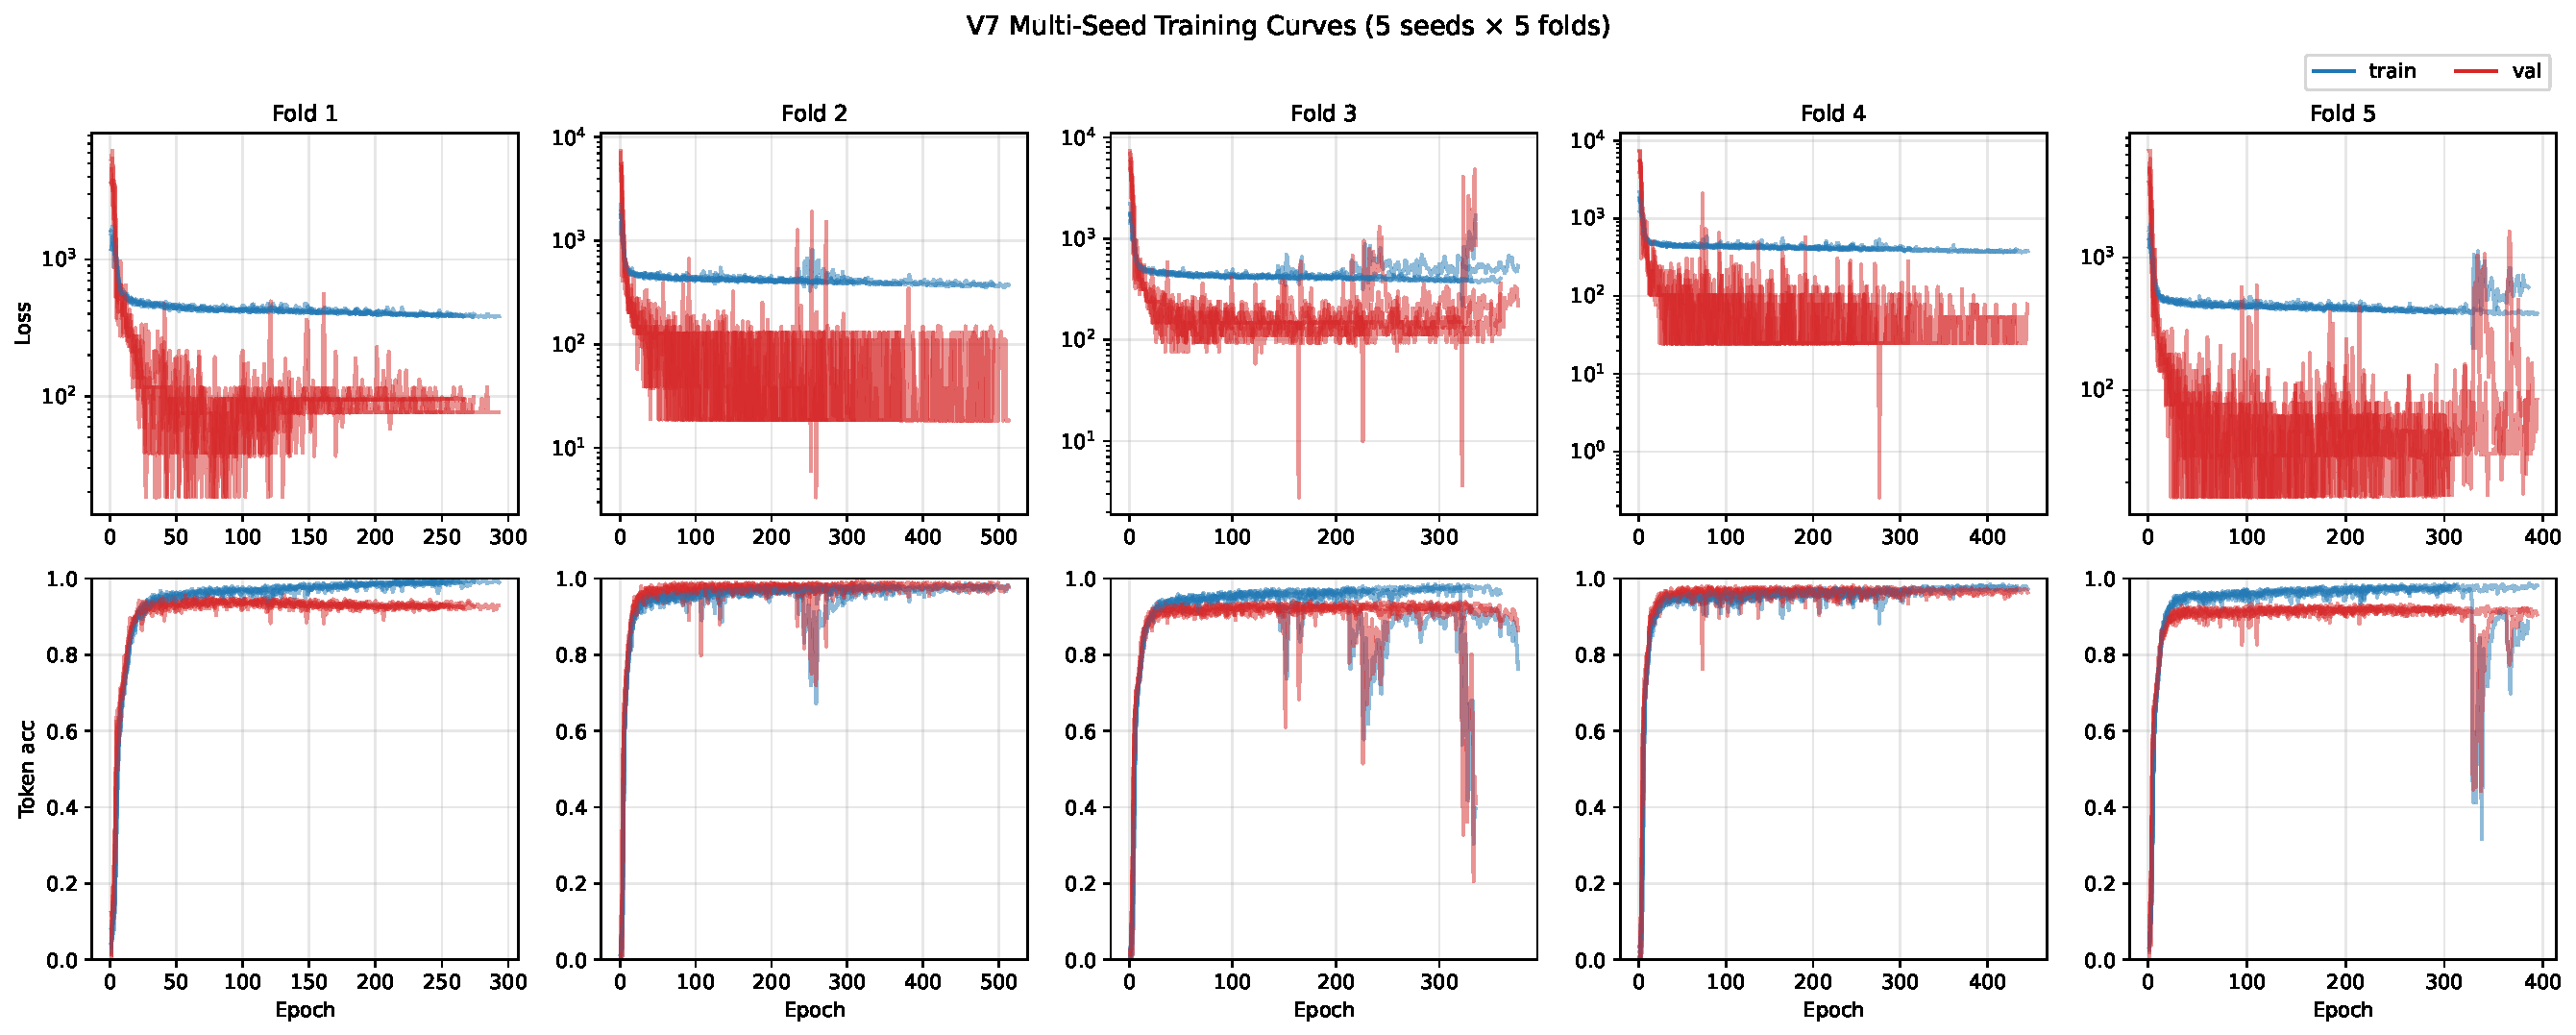
\includegraphics[width=\textwidth]{figures/training_curves_all_folds.pdf}
\caption{Training and validation curves for all 25 V7 multi-seed runs (5 folds $\times$ 5 seeds). Top row: log-scale loss. Bottom row: token accuracy. Train curves in blue, val curves in red; each panel overlays the 5 seeds for that fold. Fold~1 (leftmost) shows the largest train-val gap at $\sim$6\%; all other folds show gaps below 1.5\%. Mean final train-val token-accuracy gap across all 25 runs: 2.5\% (median 1.4\%). This near-zero gap on a 22.1M-parameter decoder trained on 545 windows is the primary evidence that the binding constraint is the encoder's sensor representation, not decoder capacity.}
\label{fig:training_curves_all}
\end{figure}

% fold_variance and ablation_fold_heatmap removed (redundant with Tables 7 and 9)

\begin{figure}[htbp]
\centering
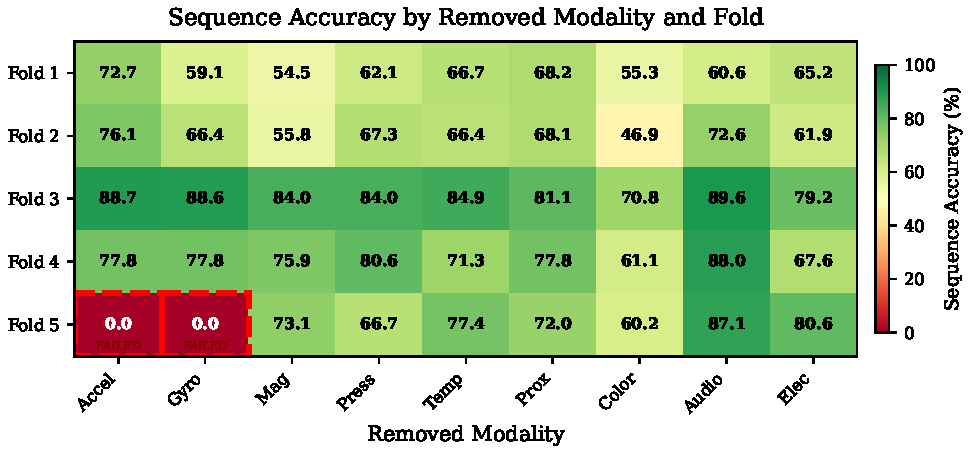
\includegraphics[width=\textwidth]{figures/fold_modality_heatmap.pdf}
\caption{Fold $\times$ modality interaction. Two catastrophic failures (Fold~5 without gyroscope or accelerometer) indicate degenerate encoder representations for specific fold/modality combinations. Audio removal shows the smallest and most uniform degradation.}
\label{fig:fold_modality}
\end{figure}

% window_fold_heatmap removed (redundant with Table 12)

\begin{figure}[htbp]
\centering
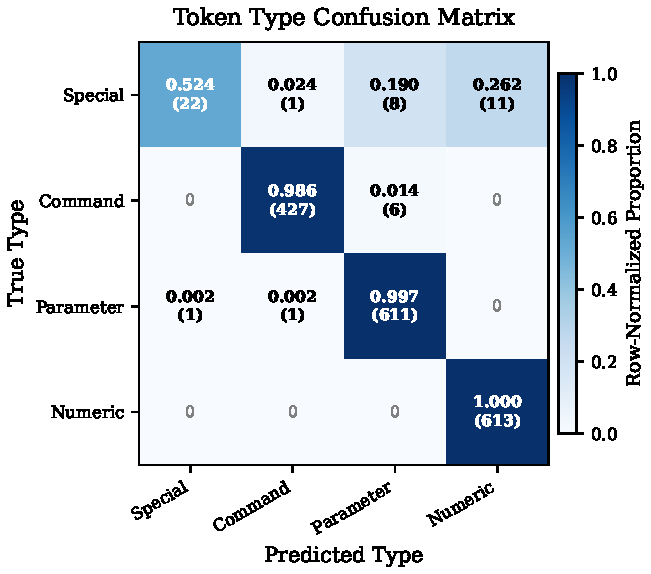
\includegraphics[width=0.75\textwidth]{figures/token_type_confusion.pdf}
\caption{Token-type confusion matrix (all 552 test windows). Numeric tokens are classified with perfect type accuracy (1.000). Command tokens occasionally scatter to Parameter (0.014). The rare Special$\to$Numeric confusion (0.262) occurs at sequence boundaries where EOS is predicted late.}
\label{fig:token_type_confusion}
\end{figure}

\begin{figure}[htbp]
\centering
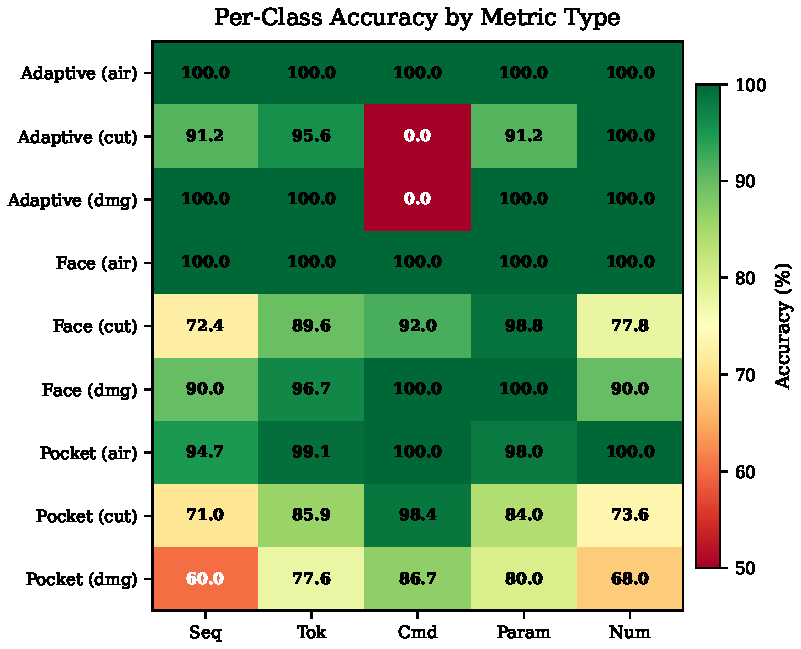
\includegraphics[width=\textwidth]{figures/per_class_metric_heatmap.pdf}
\caption{Per-class $\times$ metric heatmap. Air-cutting classes achieve 100\% across all metrics. Degradation in active-cutting and damaged-spindle classes concentrates in sequence and numeric accuracy. Cells showing ``n/a'' for command accuracy reflect modal persistence: the G-code line contains no explicit command token, so the metric is undefined for that class.}
\label{fig:per_class_metric}
\end{figure}

\begin{figure}[htbp]
\centering
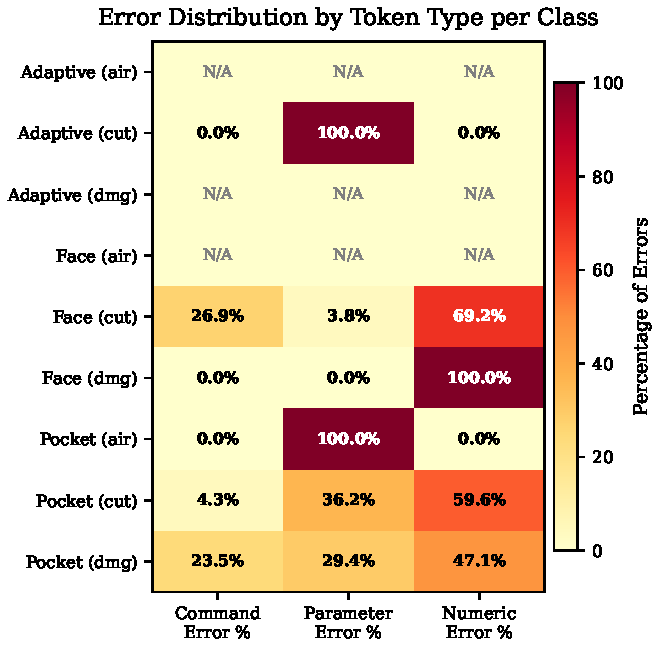
\includegraphics[width=0.85\textwidth]{figures/error_type_per_class.pdf}
\caption{Error type distribution per class (classes with zero errors omitted). Numeric errors dominate face and pocket classes; parameter errors dominate adaptive active-cut.}
\label{fig:error_type}
\end{figure}

\begin{figure}[htbp]
\centering
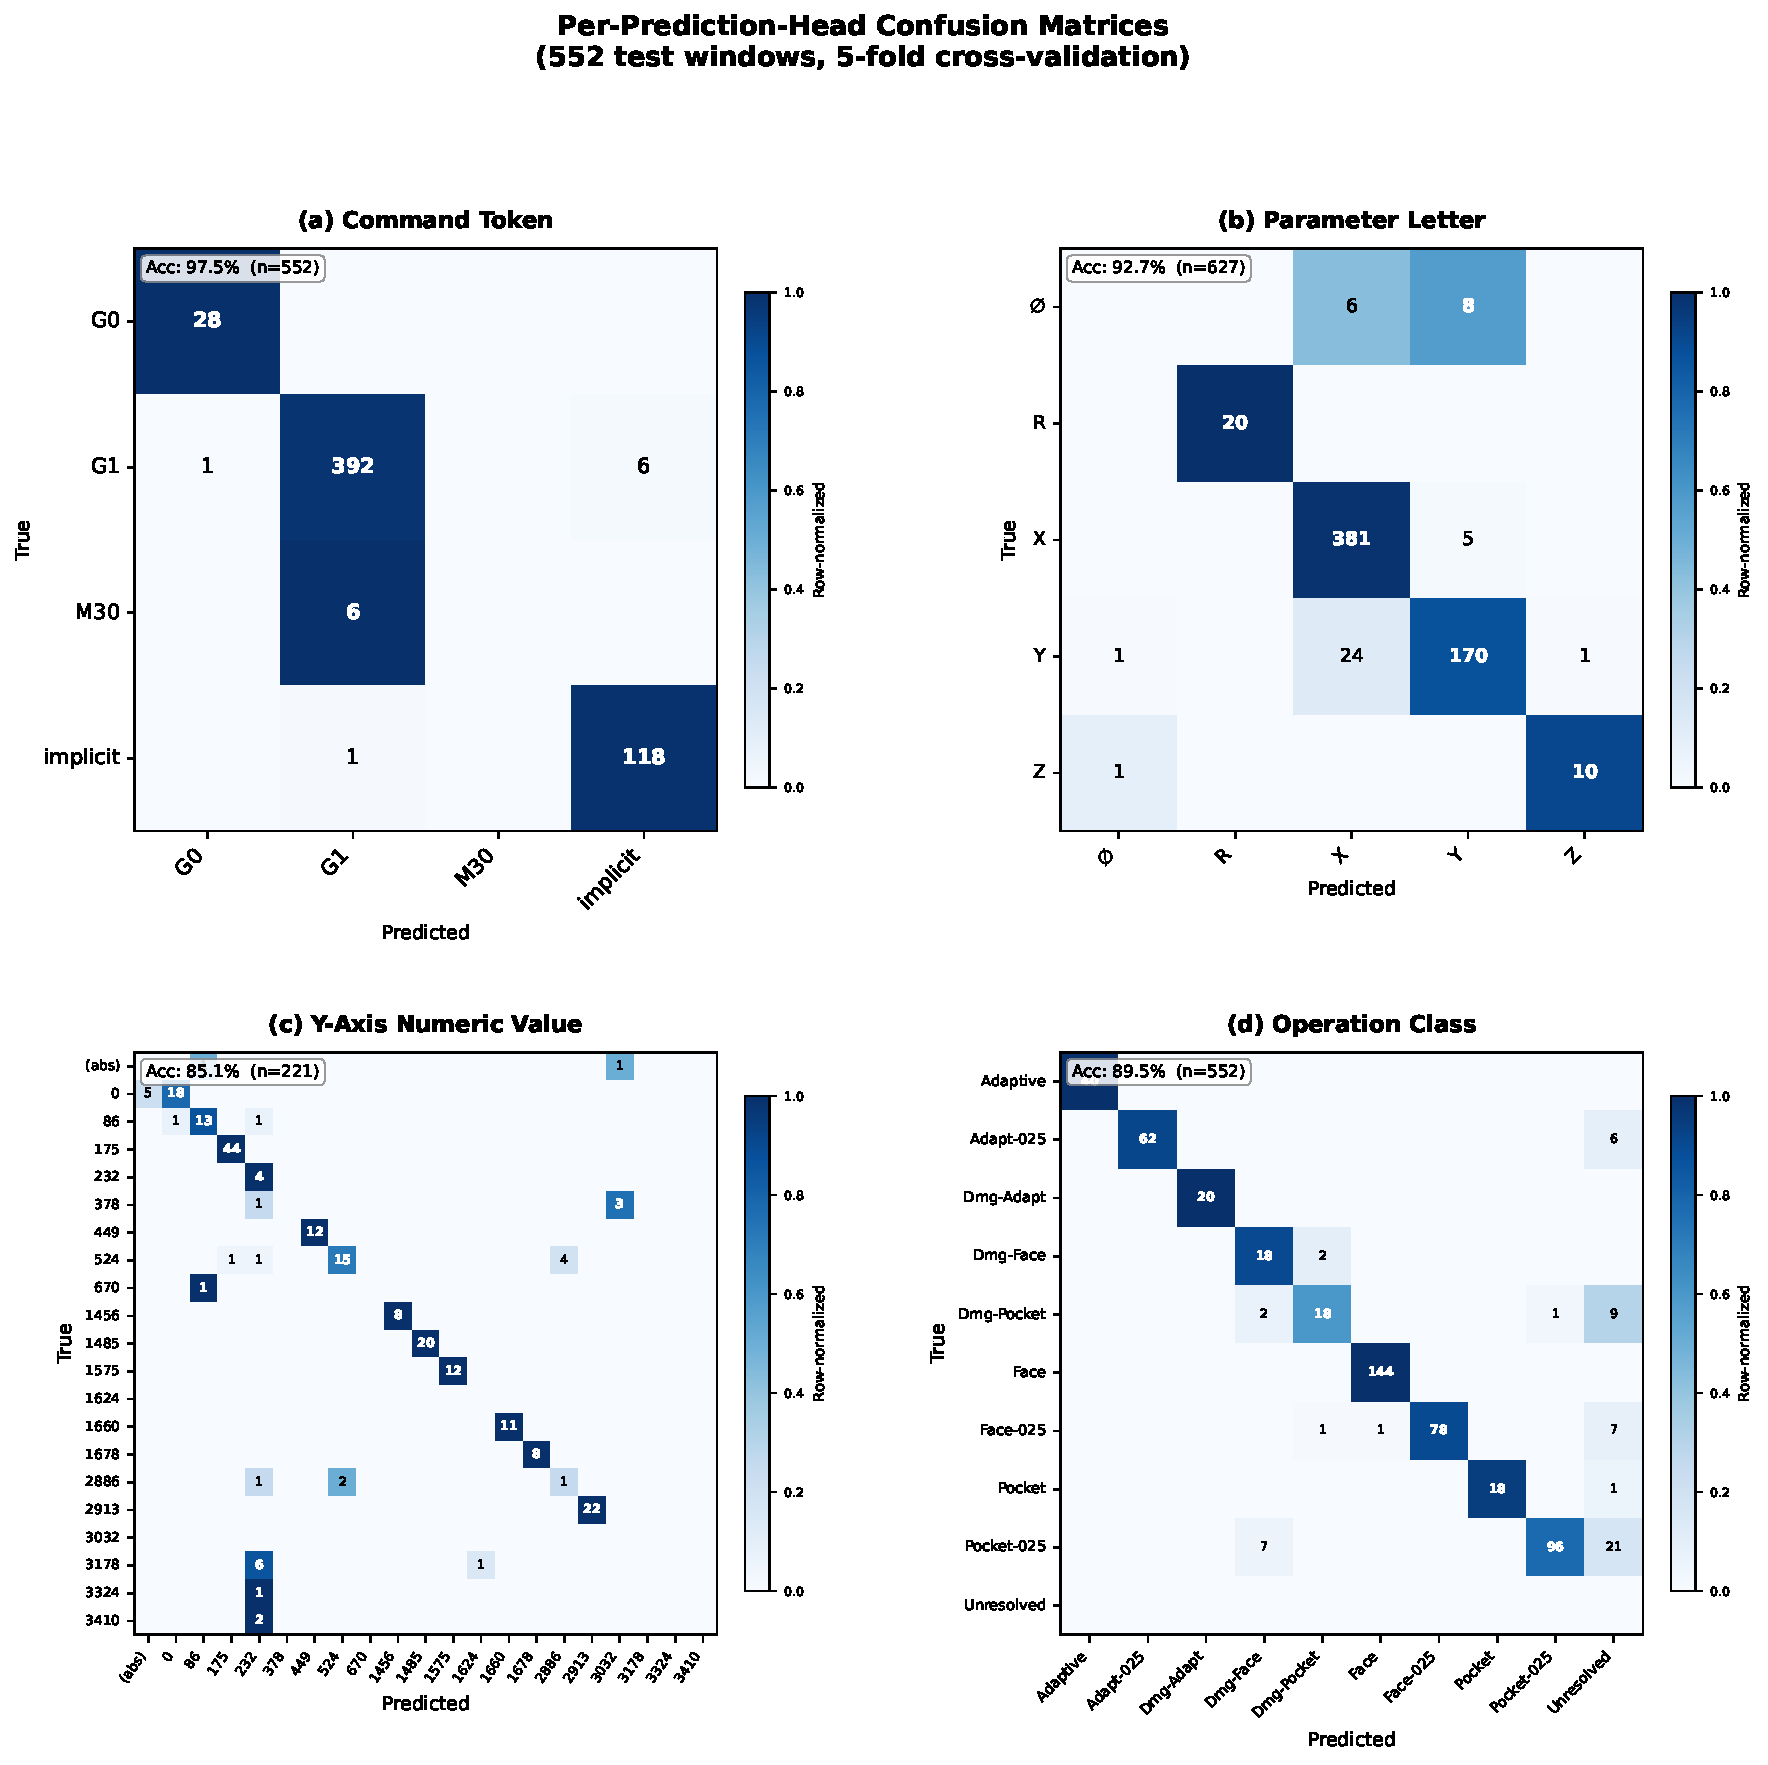
\includegraphics[width=\textwidth]{figures/per_head_confusion.pdf}
\caption{Per-head confusion matrices across all 552 test windows (V7 best config, 5 folds). \textbf{(a)}~Command tokens: 97.5\% accuracy; M30 is the only systematically misclassified command. \textbf{(b)}~Parameter letters: 92.7\% accuracy; the dominant error is Y predicted as X (24 cases). \textbf{(c)}~Y-axis numeric values: 85.1\% accuracy---the hardest head, confirming that Y-axis step-over confusion is the reconstruction bottleneck. \textbf{(d)}~Operation class: 89.5\% of predictions resolve to a known target sequence; pocket machining under active cutting contributes the most errors.}
\label{fig:per_head}
\end{figure}

\begin{figure}[htbp]
\centering
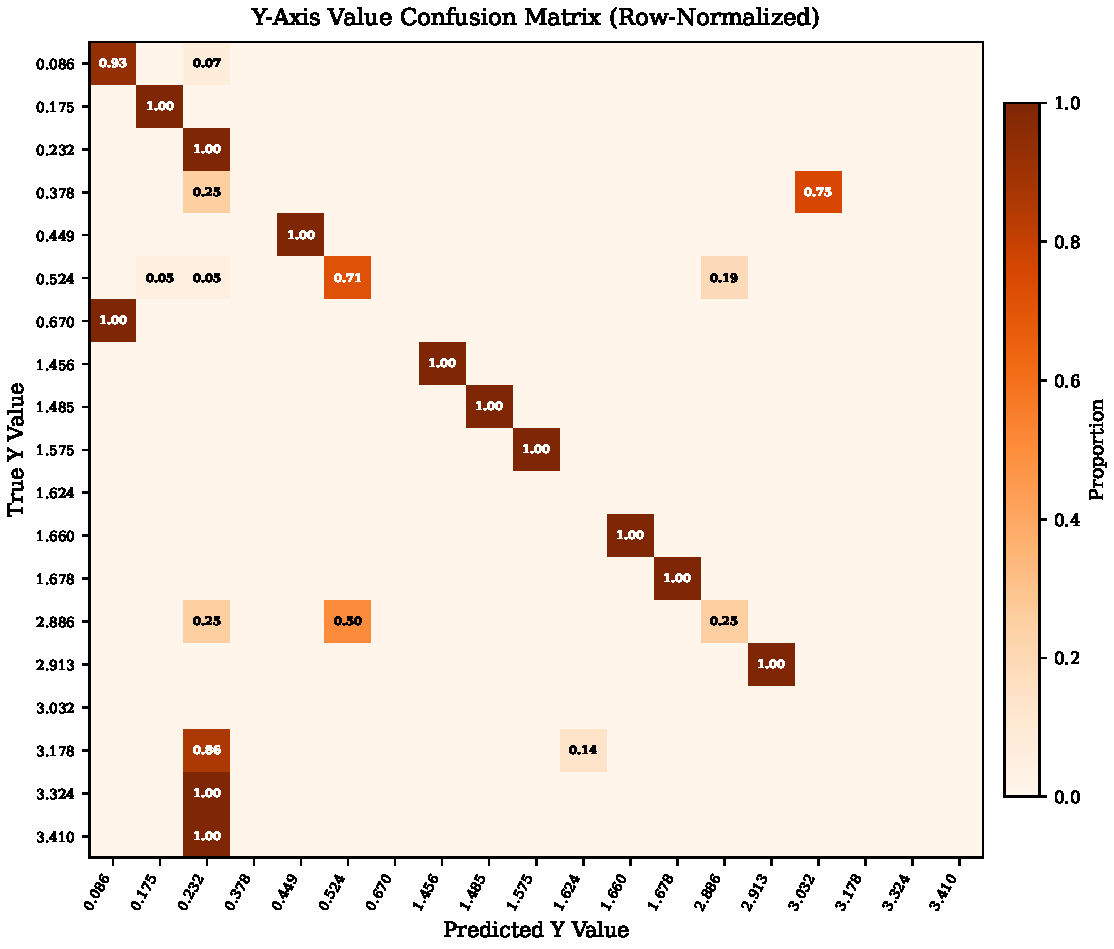
\includegraphics[width=0.85\textwidth]{figures/y_value_confusion.pdf}
\caption{Y-axis numeric value confusion matrix (row-normalized). Most Y-values are predicted correctly (strong diagonal). The primary confusion pattern is between step-over values at similar lateral positions: $Y{=}0.378$ is frequently predicted as $Y{=}3.324$, and $Y{=}0.524$ splits across $Y{=}0.086$ and $Y{=}0.175$. These confusions correspond to passes at nearby Y-coordinates where the measured dynamics are nearly identical.}
\label{fig:y_confusion}
\end{figure}

\section{Sweep Details and Supplementary Feature Analyses}
\label{sec:appendix_sweep}

This appendix provides the detailed sweep-by-sweep narrative and feature analyses that informed the final V7 configuration presented in the main text.

\subsection{V1--V7 Phase Narrative}

\textbf{Phase 1: Training sufficiency (V1$\to$V3, +16.3 pp).} The jump from 59.9\% to 76.2\% was primarily driven by longer training (100$\to$500 epochs) allowing deeper models ($n_\text{layers} = 8$) to converge, and cross-validation revealing that single-fold evaluation was both optimistic for some folds and pessimistic for others.

\textbf{Phase 2: Temporal context (V3$\to$V5, +10.2 pp).} Memory positional encoding and multi-window context provide the largest architectural improvement. In V5 (before window position was available), the combination achieves Cohen's $d = 1.09$ against the no-context baseline---a large effect size. Note that this $d$ was measured with V5's buggy random-neighbor MWC; the V7 ablation (Table~\ref{tab:ablations}) shows the corrected MWC contributes only $-$2.8~pp once window position is present.

\textbf{Phase 3: Data pipeline correctness (V5$\to$V7, +5.0 pp best, +36 pp median).} V6 regressed to 79.0\% because three high-impact data features were structurally blocked by missing metadata in preprocessed files. V7 re-processed data from raw CSVs, unblocking all three. The result is the largest improvement in \emph{robustness}: the median sequence accuracy rose from 33\% (V5) and 48\% (V6) to 84\% (V7), meaning that nearly every hyperparameter configuration now produces a viable model.

\subsection{Best Test Sequence Accuracy by Fold}

\begin{table}[htbp]
\centering
\caption{Best Test Sequence Accuracy (\%) by Fold}
\label{tab:folds}
\small
\begin{tabular}{@{}lcccccc@{}}
\toprule
& Fold 1 & Fold 2 & Fold 3 & Fold 4 & Fold 5 & Spread \\
\midrule
V5 & 63.6 & 86.4 & 81.0 & 79.0 & 65.6 & 22.8 \\
V6 & 59.8 & 72.7 & 79.0 & 65.7 & 52.7 & 26.3 \\
\textbf{V7}$^\ast$ & \textbf{73.5} & \textbf{89.4} & \textbf{86.8} & \textbf{88.9} & \textbf{91.4} & \textbf{17.9} \\
\bottomrule
\multicolumn{7}{@{}l}{\scriptsize $^\ast$V7 row: best trial across all 157 sweep configurations per fold.}\\
\multicolumn{7}{@{}l}{\scriptsize Table~\ref{tab:v7_5fold} reports the single best config retrained with}\\
\multicolumn{7}{@{}l}{\scriptsize multiple seeds (slightly different per-fold values due to seed variance).}
\end{tabular}
\normalsize
\end{table}

\subsection{V7 Sweep Metrics}

Table~\ref{tab:v7_metrics} summarizes the final results across all 157 completed V7 trials.

\begin{table}[htbp]
\centering
\caption{V7 Test-Set Metrics (157 trials, best per metric across all folds)}
\label{tab:v7_metrics}
\small
\begin{tabular}{@{}lcccc@{}}
\toprule
\textbf{Metric} & \textbf{Best} & \textbf{Median} & \textbf{Mean} & \textbf{Min} \\
\midrule
Sequence acc. & \textbf{91.4} & 84.1 & 81.5 & 63.6 \\
Token acc.    & \textbf{97.9} & 95.2 & 93.8 & 84.6 \\
Numeric acc.  & \textbf{95.7} & 92.3 & 89.9 & 76.6 \\
Command acc.  & \textbf{100.0} & 97.7 & 98.2 & 82.4 \\
Param.\ type acc. & \textbf{99.2} & 97.2 & 96.6 & 91.5 \\
\bottomrule
\end{tabular}
\normalsize
\end{table}

\subsection{Converged Hyperparameters}
\label{sec:appendix_hyperparams}

\begin{table}[htbp]
\centering
\caption{Converged Hyperparameters. Values locked after the indicated sweep and fixed for all subsequent experiments.}
\label{tab:converged}
\small
\begin{tabular}{@{}lcc@{}}
\toprule
\textbf{Parameter} & \textbf{Value} & \textbf{Locked at} \\
\midrule
$d_\text{model}$ & 384 & V2 \\
Learning rate & $3 \times 10^{-4}$ & V6 \\
Batch size & 32 & V2 \\
Dropout & 0.1 & V2 \\
Focal $\gamma$ & 2.0 & V3 \\
Memory pos.\ enc. & True & V5 \\
Window position & True & V7 \\
Sensor value prior & True & V7 \\
Hierarchical & False & V6 \\
Regression head & False & V6 \\
Seq.\ classifier & False & V6 \\
Pointer network & False & V7 \\
Noise injection & 0.0 & V6 \\
\bottomrule
\end{tabular}
\normalsize
\end{table}

Notably, the learning rate shifted from $5 \times 10^{-4}$ (optimal at 100--500 epochs in V1--V5) to $3 \times 10^{-4}$ (optimal at 500+ epochs in V6--V7). The pointer network and drop path regularization show no benefit in V7 and are locked OFF.

\subsection{Grammar Constraint Analysis}
\label{sec:appendix_grammar}

Grammar constraints underwent significant revision between V5 and V6. Initial rules (V5) prohibited command-less sequences, penalizing the common modal-persistence pattern where a G-code line begins directly with a parameter (\eg, \texttt{X3.291 Z0.0003} under implicit G1). After correcting the type-transition mask to allow \textsc{BOS}$\to$\textsc{Parameter} and \textsc{Numeric}$\to$\textsc{Command} transitions (Table~\ref{tab:grammar}):

\begin{table}[htbp]
\centering
\caption{Grammar Constraint Effect (V6, f110\_w256, $n = 309$)}
\label{tab:grammar}
\small
\begin{tabular}{@{}lccc@{}}
\toprule
& \textbf{Best} & \textbf{Mean} & \textbf{Verdict} \\
\midrule
Grammar ON  & 79.0\% & 54.7\% & Top trial \\
Grammar OFF & 78.1\% & 56.3\% & Higher mean \\
\bottomrule
\end{tabular}
\normalsize
\end{table}

The fixed grammar helps the best-tuned models achieve higher peaks but slightly hurts the average. This is consistent with the observation in~\cite{grammar_paper} that hard constraints can propagate commitment errors: if the model commits to G2, the grammar forces an R prediction that may be wrong, whereas an unconstrained model could recover by not predicting R at all.

\subsection{V5 Feature Flag Analysis}

\begin{table}[htbp]
\centering
\caption{Feature Flag Analysis (V5, f110\_w256 encoder, $n = 117$)}
\label{tab:features}
\small
\begin{tabular}{@{}lcccc@{}}
\toprule
\textbf{Feature} & \textbf{Best ON} & \textbf{Best OFF} & \textbf{Mean $\Delta$} & \textbf{$d$} \\
\midrule
MWC + MPE$^\ast$       & 86.4 & 70.5 & +14.1 & 1.09 \\
Memory pos.\ enc.     & 86.4 & 70.5 & +6.2 & 0.65 \\
Grammar constraint     & 78.1 & 86.4 & +0.0 & 0.00 \\
Hierarchical           & 86.4 & 81.0 & +0.1 & 0.01 \\
Regression head        & 81.0 & 86.4 & $-$1.3 & $-$0.13 \\
\bottomrule
\multicolumn{5}{@{}l}{\scriptsize $^\ast$MWC $k{=}1$ combined with memory positional encoding.}\\
\multicolumn{5}{@{}l}{\scriptsize $d$ = Cohen's $d$ on mean test\_seq across trials.}
\end{tabular}
\normalsize
\end{table}

Key findings: MWC + memory positional encoding is the dominant combination ($d = 1.09$); grammar constraints are neutral on average; hierarchical conditioning is redundant with memory positional encoding; regression heads are slightly harmful ($-$1.3\% mean).

\subsection{V7 Feature Flag Analysis}

\begin{table}[htbp]
\centering
\caption{V7 Feature Analysis (157 trials, all folds)}
\label{tab:v7_features}
\small
\begin{tabular}{@{}lccl@{}}
\toprule
\textbf{Feature} & \textbf{Best ON/OFF} & \textbf{Mean $\Delta$} & \textbf{Verdict} \\
\midrule
Sensor prior   & 91.4 / 91.4 & $-$0.7 & Neutral \\
Pointer network & 91.4 / 91.4 & +0.3 & Neutral \\
Grammar constr. & 91.4 / 91.4 & +0.9 & Slight positive \\
Drop path 0.1  & 91.4 / 91.4 & $-$1.7 & Slight negative \\
MWC $k{=}1,2$  & 91.4 / ---  & --- & All trials use MWC \\
\bottomrule
\end{tabular}
\normalsize
\end{table}

With 157 completed trials, no V7 feature flag shows a statistically significant effect on best accuracy---all achieve 91.4\% regardless of setting. This convergence confirms that the preprocessing fixes dominate: once the correct metadata is available, the decoder achieves strong performance regardless of architectural embellishments.

\subsection{Killed Features}

Two features were tested in V6 and permanently removed:

\textbf{Sequence classifier} (V6): A 34-class head predicting the entire G-code sequence as a classification target, intended as a prior for the autoregressive decoder. Effect: severely negative ($-$9.7\%, best 59.1\% vs.\ 79.0\% without). The classifier's global prediction interfered with the decoder's left-to-right token generation rather than guiding it.

\textbf{Noise injection} (V6): Gaussian noise ($\sigma \in \{0.01, 0.05\}$) added to encoder memory as data augmentation. Effect: negative at all levels tested. The frozen encoder already incorporates a denoising reconstruction objective~\cite{encoder_paper}; additional noise in the decoder's input degraded an already-compressed representation without providing regularization benefit.

\begin{abbreviations}
\noindent
\begin{tabular}{@{}ll}
ANOVA & Analysis of Variance \\
ASR & Automatic Speech Recognition \\
BOS & Beginning of Sequence \\
BPE & Byte Pair Encoding \\
CAM & Computer-Aided Manufacturing \\
CNC & Computer Numerical Control \\
CNN & Convolutional Neural Network \\
DTAE & Denoising Temporal Attention Encoder \\
EOS & End of Sequence \\
GPU & Graphics Processing Unit \\
HSS & High-Speed Steel \\
IMU & Inertial Measurement Unit \\
LLM & Large Language Model \\
LSTM & Long Short-Term Memory \\
MCCDAQ & Measurement Computing Data Acquisition \\
MLP & Multi-Layer Perceptron \\
MM-DTAE-LSTM & Multi-Modal Denoising Temporal Attention Encoder--LSTM \\
MWC & Multi-Window Context \\
MPE & Memory Positional Encoding \\
NIST & National Institute of Standards and Technology \\
PDM & Pulse Density Modulation \\
pp & Percentage Points \\
RMS & Root Mean Square \\
RPM & Revolutions Per Minute \\
UHMW-PE & Ultra-High Molecular Weight Polyethylene \\
\end{tabular}
\end{abbreviations}

% ============================================================================
\reftitle{References}

\bibliography{references}

\end{document}
